%& -shell-escape

\documentclass[11pt]{book}%

\usepackage{amsmath, amsthm}%
\usepackage{amsfonts}%
\usepackage{amssymb}%
\usepackage{graphicx}
\usepackage{wrapfig}

\usepackage{url}
\usepackage[utf8]{inputenc}

\usepackage{tikz}
\usetikzlibrary{shapes,arrows}
\usepackage{pgfplots}

\usepackage{slashbox}

\usepackage[left=2cm,top=2cm,right=2cm]{geometry}

\newcommand{\citep}[1]{\cite{#1}}
\def\st{\mbox{s.c. }}
\def\si{ \mbox{ si }}

\usepackage{quotchap}

%----------------------------------------------------------
\theoremstyle{plain}
\newtheorem{acknowledgement}{Acknowledgement}
\newtheorem{algorithm}{Algorithm}
\newtheorem{axiom}{Axiom}
\newtheorem{case}{Case}
\newtheorem{claim}{Claim}
\newtheorem{conclusion}{Conclusion}
\newtheorem{condition}{Condition}
\newtheorem{conjecture}{Conjecture}
\newtheorem{corollary}{Corollary}
\newtheorem{criterion}{Criterion}
\newtheorem{definition}{Definition}
\newtheorem{example}{Exemple}
\newtheorem{exercise}{Exercice}
\newtheorem{lemma}{Lemma}
\newtheorem{notation}{Notation}
\newtheorem{problem}{Problem}
\newtheorem{remark}{Remark}
\newtheorem{solution}{Solution}
\newtheorem{summary}{Summary}
\newtheorem{theorem}{Theorem}
\numberwithin{equation}{section}

\def\bx{\ensuremath{\boldsymbol{x}}}
\def\XX{\ensuremath{\mathcal{X}}}
\def\NN{\ensuremath{\mathcal{N}}}
\def\RR{\ensuremath{\mathcal{R}}}

\usepackage[T1]{fontenc}
\usepackage[frenchb]{babel}
\usepackage{mathlist}

\usepackage{enumerate}

%-----------------------------------------------------------

\begin{document}

\shorthandoff{:}

\frontmatter

\thispagestyle{empty}

\begin{center}
{\Huge \bf \sc Modèles de Recherche Opérationnelle}

\mbox{}

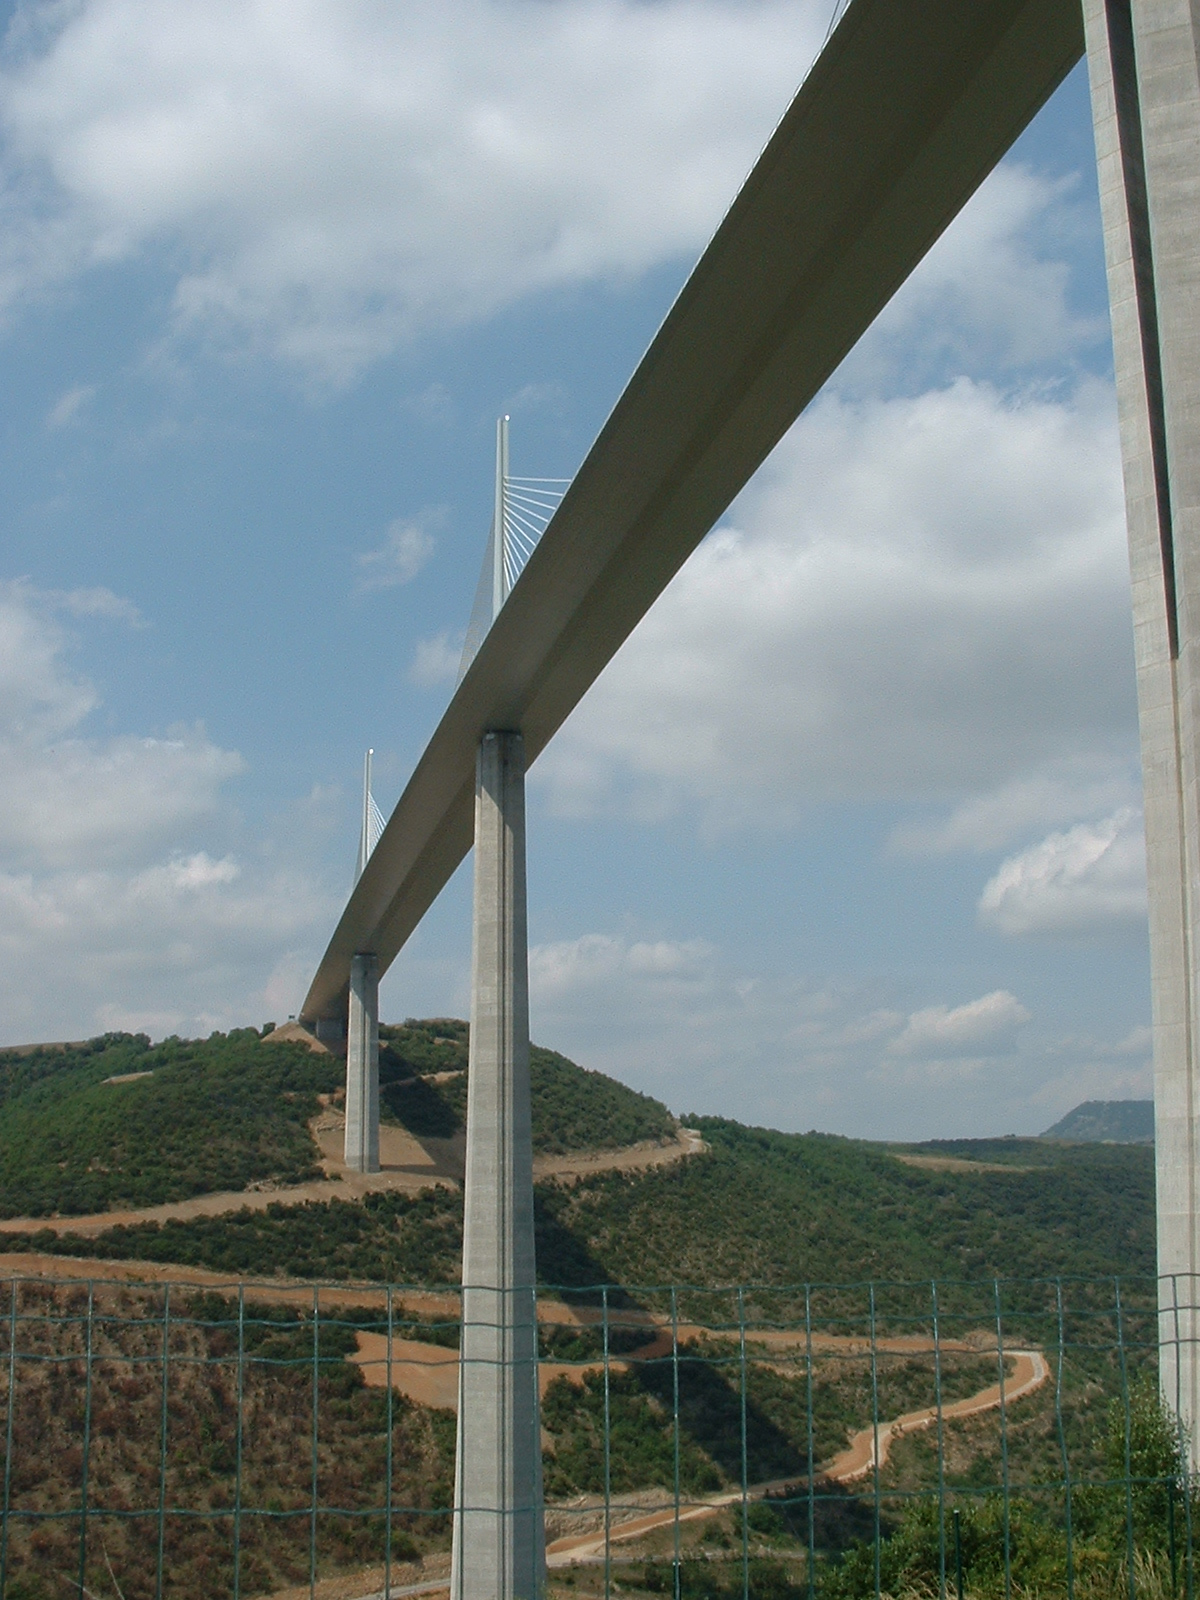
\includegraphics[width=0.7\linewidth]{dscf0035.jpg}
		
\mbox{}

{\Large Fabian Bastin}\\
{\normalsize \url{bastin@iro.umontreal.ca}}
\mbox{}\\Département d'Informatique et de Recherche Opérationnelle\\
Université de Montréal\\\mbox{}\\
\url{http://www.iro.umontreal.ca/~bastin}\\

\includegraphics[width=2cm]{cc.png}
\end{center}

\pagebreak{}

\thispagestyle{empty}

\vspace*{\stretch{1}}

\noindent
\small
La présente version de ce document s'inspire des notes de Patrice Marcotte, Bernard Gendron, ainsi que des livres {\sl Introduction to Operational Research}~\cite{HillLieb01} et {\sl The Basics of Practical Optimization}~\cite{Levy09}.

\vspace*{\stretch{1}}

{
\noindent
\footnotesize{Photographie de couverture: viaduc de Millau, France.\\
\copyright Fabian Bastin, 2006}
}

\vspace*{\stretch{1}}

\noindent

\includegraphics{cc.png}\\
Le présent document peut être modifié et redistribué à des fins non commerciales, sous conditions d'être diffusé sous les même conditions.\\
\copyright Fabian Bastin, 2015

\vspace*{\stretch{0.01}}

\tableofcontents

\mainmatter

\begin{savequote}
  OR is the art of winning wars without actually fighting.
  \qauthor{Aurther Clarke}
\end{savequote}

\chapter{Introduction}

\section{Les origines de la recherche opérationnelle}
\label{sec:histoire}

\begin{wrapfigure}{i}{0.15\textwidth}
  \begin{center}
    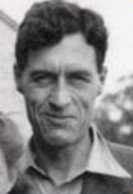
\includegraphics[width=0.14\textwidth]{Blackett-large.jpg}
  \end{center}
  \caption{Patrick Blackett}
\end{wrapfigure}

Les origines de la recherche opérationnelle, en abrégé RO, ne sont pas clairement définies, bien que Charles Babbage (1791--1871) soit souvent considéré comme le père de la recherche opérationnelle, en raison de ses travaux sur le coût du transport et le tri du courrier, menant à l'introduction du Penny Post en Angleterre, en 1840. %donner plus de détails.

Un siècle plus tard, la seconde guerre mondiale, de part son envergure, créa une besoin urgent d'allouer de manière efficace des ressources limitées aux différentes opérations militaires et aux activités au sein de chaque opération.
En particulier, l'organisation militaire britannique, puis américaine, mit à contribution un grand nombre de scientifiques pour gérer ces allocations, et s'occuper d'autres problèmes stratégiques et tactiques.
Ce faisant, ils furent appelés à poursuivre des recherches sur des opérations (militaires), et constituèrent les premières équipes de RO, notamment celle dirigée par Patrick Blackett, prix Nobel de physique en 1948~\cite{Kirb03}.
Leurs efforts furent significatifs dans la marche vers la victoire, par exemple en ce qui touche l'utilisation du radar, nouvellement développé.
Ces succès encouragèrent la poursuite de l'utilisation de la RO dans d'autres domaines.
La croissance importante de l'industrie d'après-guerre entraîna des problèmes, causés par la complexité croissante et la spécialisation dans les organisations, problèmes en fait proches de ceux présent lors du conflit.
Au début des années 1950's, la RO avait pénétré une multitude d'organisations commerciales, industrielles, et gouvernementales.
Et ce n'était que le début.

Au moins deux autres facteurs ont joué un rôle clé dans la croissance rapide de la RO.
Tout d'abord, des progrès substantiels ont été obtenus très tôt afin d'améliorer les techniques de RO.
Ces techniques, dans leur mise en pratique, furent soutenues par l'essor des outils informatiques.

\section{La nature de la recherche opérationnelle}
\label{sec:nature_ro}

``Rechercher sur des opérations'' touche tous les problèmes reliés à la conduite et à la coordination des opérations (activítés) au sein d'une organisation.
Cette organisation peut représenter des domaines très divers: l'industrie manufacturière, le transport, la construction, les télécommuncations, la finance, les soins de santé,\ldots.
La RO, associée à la révolution informatique, pénètre pratiquement tous les secteurs d'activités de la vie courante, même si sa présence est souvent invisible.

La première étape de la ``recherche'' est l'observation attentive du problème et sa formulation, ainsi que la collecte de données associées.
Il convient par la suite de construire un modéle scientifique qui tente l'abstraire l'essence du problème réel.
Tout modèle est une simplification de la réalité, mais cette représentation doit être suffisamment précise pour capturer les caractéristiques essentielles de la situation, et de pouvoir tirer des conclusions valides pour le problème réelle.
Il conviendra dès lors de tester ce modèle, et de le modifier au besoin.

Une caractéristique additionnelle est que la RO essaye souvent de trouver la meilleure solution (dite solution optimale) pour le problème examiné.
Cette solution peut ne pas être unique.
Cette recherche d'optimalité est un thème important en RO, même si son interprétation en terme managériels peut être délicate.
Il est difficile pour un individu de pouvoir maîtriser tous les aspects du problèmes à l'étude, de sorte que la RO est généralement plus un travail d'équipe, avec des experts en mathématiques, statistiques et probabilités, ingénierie, économie, administration, informatique, physiques, sciences comportementales, et les techniques spécifiques de la RO.

\section{Modélisation}
\label{sec:modeles}

Un modèle, telle que considéré dans ce cours, est une construction mathématique utilisée pour représenter certains aspects significatifs de problèmes du monde réel.
Il y a beaucoup de types différents de modèles mathématiques, mais nous nous focaliserons dans un premier temps sur les modèles d'optimisation.
Il y a trois composantes principales dans un modèle d'optimisation:
\begin{description}
\item[Variables:] elles représentent les composantes du modèle qui peuvent être modifiées pour créer des configurations différentes.
\item[Contraintes:] elles représentent les limitations sur les variables.
\item[Fonction objection]: cette fonction assigne une valeur à chaque configuration différente. Le terme ``objectif'' vient du fait que l'objectif est d'optimiser cette fonction.
\end{description}

\begin{example}[Un exemples de décisions binaires (oui/non)]
\label{sec:ex_villes}

Un étudiant en quête d'une université projette de visiter les campus de trois universités du Maine au cours d'un voyage unique, débutant et finissant à l'aéroport de Portland.
Les trois établissements sont dans les villes de Brunswick, Lewiston, et Waterville, et l'étudiant ne veut visiter chaque ville qu'une seule fois, tout en maintenant le trajet total le plus court possible.
Les distances entre ces villes sont données dans la Table~\ref{tab:distances}.

\begin{table}[htbp]
\begin{center}
\begin{tabular}{|c|c|c|c|c|}
\hline
Ville & Portland & Brunswick & Lewiston & Waterville \\
\hline
Portland & 0 & 26 & 34 & 78 \\
\hline
Brunswick & 26 & 0 & 18 & 52 \\
\hline
Lewiston & 34 & 18 & 0 & 51 \\
\hline
Waterville & 78 & 52 & 51 & 0 \\
\hline
\end{tabular}
\caption{Distances entre les villes (miles)}
\label{tab:distances}
\end{center}
\end{table}

L'étape la plus importante dans la construction d'un modèle est le choix des variables qui vont entrer en jeu.
Dans le présent cas, puisque n'importe quel trajet consiste en une série de petits déplacements entre deux villes, il est raisonnable d'assigner des variables aux décisions de partir ou non d'une ville vers une autre.
Pour plus de faciliter, numérotons les villes comme suit: 1 pour Portland, 2 pour Brunswick, 3 pour Lewiston et 4 pour Waterville. 
Ainsi, nous aurons une variable $x_{1,2}$ égale à 1 si l'étudiant voyage de Portland à Brunswick au cours de son parcours total, et 0 sinon.
Puisqu'il n'y a pas de voyage d'une ville vers cette même ville, nous avons d'ores et déjà les contraintes
\begin{equation}
x_{i,i} = 0,\ i = 1,\ldots,4.
\label{eq:dist_const_1}
\end{equation}
Une fois les variables choisies, nous pouvons essayer de formuler le problème.
Ce processus est en fait souvent une manière utile pour guider le choix des variables.

Chaque ville ne devant être visitée qu'une seule fois, elle ne peut apparaître qu'une seule fois comme ville d'arrivée.
En d'autres termes, pour $j$ fixé, $x_{i,j}$ ne peut être non-nul que pour un $i$ donné, avec $i \ne j$.
Une manière plus simple d'encoder cette information est d'écrire, pour $j = 1,\ldots,4$,
\[
x_{1,j} + x_{2,j} + x_{3,j} + x_{4,j} = 1,
\]
ou de manière plus concise.
\begin{equation}
\sum_{i = 1}^4 x_{i,j} = 1,\ j = 1,\ldots,4.
\label{eq:dist_const_2}
\end{equation}
Les contraintes formulées jusqu'à présent ne garantissent aucune forme de trajet ayant même départ et arrivée.
Par exemple, l'affectation $x_{1,2} = 1$, $x_{1,3} = 1$, $x_{1,4} = 1$, $x_{2,1} = 1$, et toutes les autres variables égales à 0, satisfont les contraintes~\ref{eq:dist_const_1} et \ref{eq:dist_const_2}.
Cette solution décrit toutefois un schéma de visites impossible puisque Portland est l'origine de tous les déplacements aux trois autres villes universitaires, mais n'est destination que depuis Brunswick.
Nous avons évidemment aussi besoin des contraintes
\begin{equation}
\sum_{j = 1}^4 x_{i,j} = 1,\ i = 1,\ldots,4,
\label{eq:dist_const_3}
\end{equation}
afin d'assurer que chaque ville ne serve d'origine que pour exactement un déplacement vers une autre ville.
Finalement, afin d'obtenir un véritable trajet ayant même origine et départ, nous devons rejeter les affectations qui décrivent des groupes déconnectés de petits déplacements comme $x_{1,2} = x_{2,1} = 1$, $x_{3,4} = x_{4,3} = 1$, avec toutes les autres variables égales à 0.
Nous pouvons forcer ceci avec les contraintes
\[
x_{i,j} + x_{j ,i} \leq 1,\ i = 1,\ldots, 4,\mbox{ et }j = 1,\ldots,4.
\]
Cette contrainte exclut tout mini-cycle.
%Exercise 1.1.2. Explain why we should not instead use the equation constraint xi, j +x j ,i = 1.

Les contraintes définies, nous devons décrire la distance totale associée à n'importe quel parcours autorisé.
Puisque nos variables ont seulement comme valeurs possibles 0 ou 1, nous pouvons multiplier chacune d'elle par la distance correspondante entre les deux villes indexées, et les additionner:
\[
\sum_{i = 1}^4 \sum_{j = 1}^4 x_{i,j} a_{i,j}.
\]
Notre modèle mathématique consiste à minimiser cette fonction, dite {\sl fonction objectif} par rapport aux variables $x_{i,j}$, tout en satisfaisant les contraintes préalablement décrites:
\begin{align*}
\min_x \ & \sum_{i = 1}^4 \sum_{j = 1}^4 x_{i,j} a_{i,j}, \\
\mbox{s.c.} \ & x_{i,i} = 0,\ i = 1,\ldots, 4, \\
& \sum_{i = 1}^4 x_{i,j} = 1,\ j = 1,\ldots,4, \\
& \sum_{j = 1}^4 x_{i,j} = 1,\ i = 1,\ldots,4, \\
& x_{i,j} + x_{j ,i} \leq 1,\ i = 1,\ldots, 4,\mbox{ et }j = 1,\ldots,4,\\
& x_{i,j} \in \lbrace 0, 1 \rbrace, \ i = 1,\ldots, 4,\mbox{ et }j = 1,\ldots,4.
\end{align*}
Ici, $x = (x_{i,j})_{i = 1,\ldots, 4, j = 1,\ldots,4}$, et {\sl s.c.}, ``sous les contraintes''.
Le problème d'optimisation ainsi construit constitue un {\sl programme mathématique}.

%\subsubsection{Résolution du programme mathématique}

Le problème de visites d'universités est assez petit que pour être résolu explicitement, sans recourir à des méthodes d'optimisation numérique.
Puisqu'il y a seulement trois parcours significativement différents, la distance totale associée à chacun d'eux pourrait être facilement calculée, et nous choisissons le parcours de longueur minimale, qui est ici
\begin{center}
Portland $\rightarrow$ Brunswick $\rightarrow$ Waterville $\rightarrow$ Lewiston $\rightarrow$ Portland.
\end{center}
avec une distance totale de 163 miles.
Il est cependant clair qu'une telle stratégie de résolution ne fonctionne plus comme le nombre de villes augmente.
\end{example}

\begin{example}[Un problème de mélange]

Un armateur doit construire un navire de guerre à partir de 50 tonnes d'acier contenant entre 0.5\% et 1.25\% de carbone (C), entre 0.3\% and 0.5\% de silicone (Si), pas plus de 0.05\% de sulfure (Su), et pas plus de 0.04\% de phosphore (Ph).
Un fournisseur produit de l'acier à partir de sept matières premières dont les qualités, les disponibilités en tonnes, et les coûts en \$/tonne sont donnés dans la Table~\ref{tab:steeldata}.
Le fournisseur veut déterminer la combinaison la moins coûteuse de composants bruts qu'il peut utiliser pour produire l'acier répondant aux besoins de l'armateur.
\begin{table}[htb]
\begin{center}
\begin{tabular}{lrrrrrr}
Matière première & \% C & \% Si & \% Su & \% Ph & Disponibilité & Coût \\
\hline
limonite & 3.0 & 0 & 0.013 & 0.015 & 40 & 200 \\
taconite & 2.5 & 0 & 0.008 & 0.001 & 30 & 250 \\
hématite & 0 & 0 & 0.011 & 0.05 & 60 & 150 \\
magnétite & 1.2 & 0 & 0.002 & 0.008 & 50 & 220 \\
silicone 1 & 0 & 90 & 0.004 & 0.002 & 20 & 300 \\
silicone 2 & 0 & 96 & 0.012 & 0.003 & 30 & 310 \\
charbon & 90 & 0 & 0.002 & 0.01 & 25 & 165 \\
\hline
\end{tabular}
\label{tab:steeldata}
\caption{Données pour le problème de production d'acier}
\end{center}
\end{table}

Puisque les fournisseur peut changer les quantités de matéries premières utilisées dans la producton de l'acier, nous pourrions assigner une variable différente pour représenter la quantiter de chaque matière première:
\begin{itemize}
\item
$x_1$ = tonnes de limonite,
\item
$x_2$ = tonnes de taconite,
\item
$x_3$ = tonnes d'hématite,
\item
$x_4$ = tonnes de magnétite,
\item
$x_5$ = tonnes de silicone 1,
\item
$x_6$ = tonnes de silicone 2,
\item
$x_7$ = tonnes de charbon.
\end{itemize}
Notons que les variables sont ici continues, contrairement à l'exemple précédent.

Afin de modéliser les contraintes, observons tout d'abord que
les variables dans ce cas sont naturellement bornées inférieurement par 0 (puisque des quantités négatives ne feraient pas de sens), et bornées supérieurement par leur quantité disponible, aussi avons-nous:
\begin{align*}
0 & \leq x_1 \leq 40, \\
0 & \leq x_2 \leq 30, \\
0 & \leq x_3 \leq 60, \\
0 & \leq x_4 \leq 50, \\
0 & \leq x_5 \leq 20, \\
0 & \leq x_6 \leq 30, \\
0 & \leq x_7 \leq 25.
\end{align*}
En supposant que n'importe quelle quantité d'une matière première contribue pour la même quantité d'acier, et en sachant que nous devons produire au moins 50 tonnes, nous avons
\[
\sum_{i = 1}^7 x_i \geq 50.
\]
Notons que nous ne supposons pas que nous produirons exactement 50 tonnes, puisqu'il peut être nécessaire de produire d'avantage afin de satisfaire les autres exigences du problème.

L'autre caractéristique contraignante dans ce problème que que l'acier doit contenir un certain pourcentage de carbone, de silicone, de sulfure et de phosphore.
Afin de voir comment ces exigences de composition se traduisent en contraintes par rapport à nos variables, nous nous concentrerons d'abord sur l'exigence d'avoir entre 0.5\% et 1.25\% de carbone, en espérant que les exigences sur le silicone, le sulfure et le phosphore se formulent de manière similaire.
À partir des données, nous connaissons le pourcentage de contribution en carbone de chaque matière première, aussi nous pouvons facilement calculer la quantité de carbone pour n'importe quel choix de variables comme
\[
0.03x_1+0.025x_2+0.012x_4+0.9x_7.
\]
Cependant, comme nous avons une exigences de proportion de carbone dans l'acier, nous devons diviser cette quantité de carbone par la quantité d'acier:
\[
\%C= 100 \left( \frac{\mbox{tonnes de carbone}}{\mbox{tonnes d'acier}} \right)
=
\frac{3.0 x_1+2.5 x_2+1.2 x_4+90 x_7}
{x_1+x_2+x_3+x_4+x_5+x_6+x_7}
.
\]
La contrainte que l'acier contienne entre 0.5\% et 1.25\% de carbone se traduit
dans la paire de contraintes
\begin{equation}
0.5 \leq
\frac{3.0 x_1+2.5 x_2+1.2 x_4+90 x_7}
{x_1+x_2+x_3+x_4+x_5+x_6+x_7}
\leq 1.25.
\label{eq:steel_composition}
\end{equation}
Les contraintes pour les autres composants se formulent de manière similaires.

Puisque ce problème implique de trouver la combinaison la moins coûteuse de matières premières qui rencontre la demande de 50 tonnes d'acier, la fonction objectif est simplement le coût des matières premières utilisées:
\[
\mbox{coût} = 200 x_1 + 250 x_2 + 150 x_3 + 220 x_4 + 300 x_5 + 310 x_6 + 165 x_7,
\]
où chaque matière première contribue pour son propre coût au total.
Le problème d'optimisation est dès lors la minimisation de cette fonction coût sur tous les choix des variables qui satisfont les contraintes modélisées.

Il n'est plus possible ici d'énumérer les solutions possibles afin de résoudre le modèle, en particuler puisque les variables considérées sont continues.
Nous pouvons néanmoins obtenir une intuition de la solution en considérant le comportement de la fonction objectif.
Ainsi, il est évident que celle-ci décroît quand une des variables diminue, et que la contribution la plus faible en termes de coût vient des variables avec les plus petits coefficients (i.e. les matières premières avec les coûts moindres par unité).
Si nous ignorons les contraintes de composition, le fournisseur devrait produire exactement 50 tonnes d'acier à partir des matières premières disponibles les moins chères.
Ceci signifierait utiliser 50 des 60 tonnes disponibles d'hématite (au coût de \$150 par tonne), pour un coût total des \$7,500.

Avant d'essayer de résoudre le problème d'optimisation complet (à l'aide d'un ordinateur), nous devrions réécrire les contraintes de composition dans une forme plus simple.
Par exemple, la contrainte \ref{eq:steel_composition} est nonlinéaire, mais peut être réexprimée comme deux contraintes linéaires en multipliant chaque terme des inégalités par le dénominateur.
Après la simplification de toutes les contraintes de composition de cette manière, et en utilisant un logiciel d'optimisation, nous obtenons la solution
\[
x_1 = 13.7888,\ x_3 = 35.8097,\ x_5 = 0.166667,\ x_7 = 0.234818,\ x_2 = x_4 = x_6 = 0,
\]
qui se traduit en exactement 50 tonnes d'acier, produit à partir de 13.7888 tonnes de limonite, 35.8097 tonnes d'hématite, 0.166667 tonnes de silicone 1 et 0.234818 tonnes de charbon.
Le coût total de production pour cette solution est \$8,217.96.
\end{example}


\section{Algorithmes et logiciels}

Au-delà de la modélisation, la résolution de problèmes de recherche opérationnelle nécessite de recourir à des algorithmes adapatés à la nature du problème, et capables de traiter de quelques dizaines à des millions de variables.
Leur étude consistera par conséquent une partie importante du présent document.
Même si de nombreux logiciels mettant en oeuvre ces algorithmes sont commerciaux, le monde de l'open-source n'est pas en reste avec notamment des projets tels que COIN-OR (\url{http://www.coin-or.org}). Il existe aussi diverses versions d'évaluations de solveurs commerciaux, ainsi que l'interface web NEOS (\url{http://www-neos.mcs.anl.gov}).
L'utilisation de tels outils nécessitent toutefois l'apprentissage de langages de modélisation adaptés; dans ce cours, nous nous baserons sur le langage GAMS (\url{http://www.gams.com}).
Ces langages servent à décrire dans des termes compréhensibles par le solveur le problème à résoudre.
La dernière version de IOR-Tutorial, développé en Java et proposé en complément à Hillier et Lieberman~\cite{HillLieb01}, peut également se révéler un complément précieux pour se familiariser avec les techniques de recherche opérationnelle.

\subsection{Un exemple avec GAMS}

GAMS est l'acronyme de General Algebric Modeling System.
Il consiste en un langage de description de problèmes, qui peut être compilé, et en une interface vers différent solveurs.
Une version gratuite de démonstration, permettant de résoudre des problèmes de petite taille, est disponible en téléchargement à l'adress \url{http://www.gams.com}.
Ce langage peut également être utilisé avec divers solveurs proposés sur NEOS.
Nous reviendrons plus en détail ultérieurement sur la formulation d'un programme mathématique avec GAMS, et nous contenterons d'un petit exemple introductif à ce stade.

Considérons un brasseur qui disposent des éléments suivants dans son stock:
\begin{enumerate}
\item
malt (75 kg);
\item
houblon (60 kg);
\item
levure (50 kg).
\end{enumerate}
Deux produits peuvent être obtenus: de la bière légère et de la bière noire.
Pour un kg de bière légère, il faut 2 kg de malt, 3 kg de houblon, et 2 kg de levure.
Pour un kg de bière noire, il faut 3 kg de malt, 1 kg de houblon, et 5/3 kg de levure.
La bière noire est vendue la moitié du prix de la bière légère.
En supposant que toute la production sera vendue, le brasseur souhaiterait décider des quantités de bières noire et légère à produire pour optimiser son profit.
Le programme GAMS résultant est
\begin{verbatim}
set b types of beer /light, dark/;

set i inputs /malt, hops, yeast/

parameter r(i) raw supplies /malt 75, hops 60, yeast 50/;

table a(i,b) input requirements

      light dark
malt  2     3
hops  3     1
yeast 2     1.67

parameter p(b) selling price / light 2, dark 1/;

variables pi profit (maximand)
          x(b) production level;

equations profit defines gross revenue
          supply(i) input supply constraint;

profit..     pi =e= sum(b, p(b) * x(b));
supply(i)..  sum(b, a(i,b)*x(b)) =L= r(i);

model beer /all/;

x.lo(b) = 0;

solve beer using lp maximizing pi;
\end{verbatim}

\begin{small}
\section{Notes}

Le contenu des Section~\ref{sec:histoire} et \ref{sec:nature_ro} se base principalement sur Hillier et Lieberman~\cite{HillLieb01}, Chapitre~1. La Section~\ref{sec:modeles} est construite à partir du Chapitre~1 de Levy~\cite{Levy09}. L'exemple GAMS est dû à Thomas F. Rutherford.

\end{small}


\chapter{Programmation linéaire}

\section{Introduction}

Bien que la réalité soit souvent loin d'être linéaire, un grand nombre de problèmes peuvent s'écrire sous forme linéaire, soit directement, soit en première simplification.
D'autre part, un très grand nombre de modèles constituent des extensions de programmes linéaires. Sa compréhension est essentielle à la compréhension de modèles plus sophistiqués.

Un programme linéaire générique s'écrit sous la forme
\[
\begin{matrix}
\max_x & c_1x_1 & + & \ldots & + & c_n x_n \\
& a_{11}x_1 & + & \ldots & + & a_{1n} x_n & \leq b_1 \\
& \vdots & & & \vdots \\
& a_{m1}x_1 & + & \ldots & + & a_{mn} x_n & \leq b_m,
\end{matrix}
\]
ou, sous une forme plus compacte,
\begin{align*}
\max_x & \sum_{j = 1}^n c_jx_j \\
& \sum_{j = 1}^n a_{ij}x_j \leq b_i, \quad i = 1,\ldots,m.
\end{align*}
La ligne
\[
\sum_{j = 1}^n c_jx_j
\]
représente la {\sl fonction objectif}, que nous souhaitons maximiser.
La maximisation se fait en respectant les $m$ {\sl contraintes}
\[
\sum_{j = 1}^n a_{ij}x_j \leq b_i, \quad i = 1,\ldots,m.
\]

Sous forme matricielle, le problème se réecrit
\begin{align*}
\max_x\ & c^T x \\
& Ax \leq b,
\end{align*}
avec
\begin{align*}
x &= \begin{pmatrix} x_1 \\ \vdots \\ x_n \end{pmatrix}, \quad
c = \begin{pmatrix} c_1 \\ \vdots \\ c_n \end{pmatrix}, \quad
b = \begin{pmatrix} b_1 \\ \vdots \\ b_n \end{pmatrix} \\
A &= \begin{pmatrix}
a_{11} & a_{12} & \ldots & a_{1n} \\
a_{21} & a_{22} & \ldots & a_{2n} \\
a_{m1} & a_{m2} & \ldots & a_{mn}
\end{pmatrix}.
\end{align*}

La terminologie ``linéaire'' vient du fait que toutes les fonctions impliquées sont linéaires.
Typiquement, nous ajouterons également des contraintes de non-négativités:
\[
x_i \geq 0,\ i = 1,\ldots,n,
\]
ou, en abrégé,
\[
x \geq 0.
\]
Nous dirons aussi que le vecteur $x$ appartient à l'orthant positif (i.e. $x \in \RR_+^n$).

\begin{example}[Wyndor Glass]
\label{ex:wyndor}
La compagnie Wyndor Glass Co. produit des produits verriers de haute qualité, incluant des fenêtres et des portes vitrées.
Elle dispose à cette fin de trois usines (usine 1, usine 2, usine 3), qui ont chacune une capacité de production limitée.
Les châssis en aluminium et les matériaux sont produits dans l'usine 1, les châssis en bois sont fabriqués dans l'usine 2, et l'usine 3 produit le verre et assemble les produits.
La compagnie a décidé de mettre en place de ligne de production:
\begin{itemize}
\item
produit 1: une porte vitrée avec un châssis d'aluminium;
\item
produit 2: une fenêtre double-vitrage avec châssis en bois.
\end{itemize}

Un lot de 20 unités donne lieu à un profit de \$3000 et \$5000, respectivement pour le produit 1 et le produit 2. Les données du problème sont synthétisées dans la Table~\ref{tab:wyndor}.
\begin{table}[htbp]
\begin{center}
\begin{tabular}{|c|c|c|c|}
\hline
& Produit 1 & Produit 2 & Capacité de \\
& Temps de prod. (h) & Temps de prod. (h)& production (h)\\
\hline
Usine 1 & 1 & 0 & 4 \\
\hline
Usine 2 & 0 & 2 & 12 \\
\hline
Usine 3 & 3 & 2 & 18 \\
\hline
\end{tabular}
\end{center}
\caption{Données du problème Wyndor Glass}
\label{tab:wyndor}
\end{table}
Chaque lot d'un produit est le résultat combiné de la production dans les trois usines.
Nous souhaitons déterminer le taux de production pour chaque produit (nombre de lots par semaine) de façon à maximiser le profit total.

Les variables de décision sont
\begin{itemize}
\item
$x_1$, le nombre de lots du produit 1;
\item
$x_2$, le nombre de lots du produit 2.
\end{itemize}
Le fonction objectif est le profit total, qui vaut $3x_1 +5x_2$, en l'exprimant en miller de dollars. Nous voulons maximiser ce profit.

Les contraintes concernent tout d'abord les capacítés de production:
\begin{eqnarray*}
x_1 & \leq 4 & \mbox{(usine 1)} \\
2x_2 & \leq 12 & \mbox{(usine 2)} \\
3x_1 + 2x_2 & \leq 18  & \mbox{(usine 3)}
\end{eqnarray*}
Viennent ensuite les contriantes de non-négativité:
\[
x_1 \geq 0, x_2 \geq 0. \qquad \mbox{(nombre positif d'unités produites)}
\]

En résumé, nous avons le problème d'optimisation suivant:
\[
\max_x z = 3x_1 + 5x_2
\]
sous les contraintes
\begin{eqnarray*}
x_1\qquad & \leq 4 & \mbox{(usine 1)} \\
 \qquad  2x_2 & \leq 12 & \mbox{(usine 3)} \\
3x_1 + 2x_2 & \leq 18 & \mbox{(usine 3)}
\end{eqnarray*}
\[
x_1 \geq 0,\ x_2 \geq 0\ \mbox{(non-négativité)}
\]

Avant de traiter de méthodes numériques, essayons de visualiser le problème afin de développer une intuition quand à sa résolution.
Le problème peut-être représenté comme sur la Figure~\ref{fig:wyndor}.
Pour le réaliser, nous traçons d'abord les droites correpondant aux contraintes, puis nous déterminons le domaine réalisable en vérifiant le sens des inégalités pour chacune d'elle.
Nous traçons ensuite les droites correspondant à la variation de l'objectif.
Dans l'exemple
\[
z = 3x_1+5x_2 \Leftrightarrow x_2 = -\frac{3}{5}x_1 + \frac{1}{5}z.
\]
L'ordonnée à l'origine, dépendant de la valeur de $z$, est $\frac{1}{5}z$, et la pente vaut $-\frac{3}{5}$.
Maximiser revient à augmenter $z$.
\begin{figure}[htbp]
\begin{center}
\begin{tikzpicture}[scale=0.75]
\draw[->] (0,0) -- (10,0) node[below,right] {$x_1$};
\draw[->] (0,0) -- (0,10) node[above,left] {$x_2$};
\draw (6,0) -- (0,9) node[above,right] {$3x_1 + 2x_2 \leq 18$};
\draw (0,6) -- (8,6) node[right] {$2x_2 \leq 12$};
\draw (4,0) -- (4,8) node[above,right] {$x_1 \leq 4$};

\foreach \x in {0,1,2,3,4,5,6,7,8,9}
  \draw (\x,1pt) -- (\x,-1pt) node[anchor=north] {$\x$};
\foreach \y in {0,1,2,3,4,5,6,7,8,9}
  \draw (1pt,\y) -- (-1pt,\y) node[anchor=east] {$\y$};

\filldraw[fill=yellow]
  (0,0) -- (0,6) -- (2,6) -- (4,3) -- (4,0) -- (0,0);
  
\draw (2,3) node[text width=2cm,text ragged] {domaine réalisable};

\end{tikzpicture}
\end{center}
\caption{exemple Wyndor Glass}
\label{fig:wyndor}
\end{figure}

\begin{figure}[htbp]
\begin{center}
\begin{tikzpicture}[scale=0.75]
\draw[->] (0,0) -- (10,0) node[below,right] {$x_1$};
\draw[->] (0,0) -- (0,10) node[above,left] {$x_2$};

\foreach \x in {0,1,2,3,4,5,6,7,8,9}
  \draw (\x,1pt) -- (\x,-1pt) node[anchor=north] {$\x$};
\foreach \y in {0,1,2,3,4,5,6,7,8,9}
  \draw (1pt,\y) -- (-1pt,\y) node[anchor=east] {$\y$};

\filldraw[fill=yellow]
  (0,0) -- (0,6) -- (2,6) -- (4,3) -- (4,0) -- (0,0);

\draw (5.0,-1) -- (-1,13.0/5) node[above,left] {$10=3x_1+5x_2$};
\draw (25.0/3,-1) -- (-1,23.0/5) node[above,left] {$20=3x_1+5x_2$};
\draw (41.0/3,-1) -- (-1,39.0/5) node[above,left] {$36=3x_1+5x_2$};

\draw (2,6) node[above] {$(2,6)$};
\fill (2,6) circle (2 pt);

\end{tikzpicture}
\end{center}
\caption{exemple Wyndor Glass: maximisation}
\label{fig:wyndor_2}
\end{figure}
\end{example}

La représentation graphique, bien qu'intéressante pour ``voir'' comment se passe les choses, ne fonctionnent plus dès que nous avons plus de deux variables.
Il faut alors passer à l'utilisation de logiciels, utilisant l'algorithme du simplexe ou de points intérieurs.
Nous n'aborderons que le premier dans le cadre de ce cours introductif.

\section{Modèle général de programmation linéaire}

Le modèle complet
\begin{align*}
\max_x\ & c^T x \\
& Ax \leq b, \\
& x \geq 0,
\end{align*}
est appelé {\sl forme standard}.
Le modèle complet
\begin{align*}
\max_x\ & c^T x \\
& Ax \leq b, \\
& x \geq 0,
\end{align*}
est appelé {\sl forme standard}.

D'autres formes sont possibles et définissent aussi des modèles de programmation linéaire:
\begin{itemize}
\item
minimiser au lieu de maximiser:
\[
\min f(x) = -\max f(x);
\]
\item
les inégalités peuvent être remplacées par des égalités, ou être de sens contraire;
\item
certaines variables peuvent ne pas être forcés à être supérieures à 0. Par exemple, considérons la contrainte
\[
x \geq -4,
\]
qui équivaut à
\[
x + 4 \geq 0.
\]
Nous pouvons alors définir $y = x+4$, de sorte que la contrainte devient
\[
y \geq 0.
\]
De même, considérons
\[
-10 \leq x \leq -2.
\]
En définissons $y = x+10$, nous avons la contrainte $y \geq 0$.
\end{itemize}

\section{Terminologie de base}

Nous parlerons de {\sl solution réalisable} à propos d'une solution (i.e. une instance particulière du vecteur $x$) pour laquelle toutes les contraintes sont satisfaites.
En d'autres termes cette solution appartient au domaine réalisable.
Par exemple, le point $(1,1)$ est une solution réalisable pour la Figure~\ref{fig:wyndor}.
A contrario, une solution non réalisable est une solution pour laquelle au moins une contrainte est violée. Elle n'appartient pas au domaine réalisable.
Une {\sl solution optimale} est une solution donnant la meilleure valeur possible pour l'objectif. Cette valeur est dite {\sl valeur optimale}.
Un modèle n'a aucune solution optimale si son domaine réalisable est vide, ou si la fonction objectif est non bornée.
Ajoutons par exemple la contrainte
\[
3x_1 + 5x_2 \geq 50
\]
dans l'exemple Wyndor Glass.
Cette nouvelle contrainte ne peut être satisfaite en même temps que les contraintes précédentes, comme illustré dans la Figure~\ref{fig:wyndor_unfeasible}.
Plus aucun point n'est réalisable.
Si nous supprimons plutôt les contraintes
\[
2x_2 \geq 12,\quad 3x_1 + 2x_2 \leq 18,
\]
la fonction objectif devient non bornée dans le domaine réalisable, comme illustré sur la Figure~\ref{fig:wyndor_unbounded}.
Un modèle peut également présenter une infinité de solutions optimales.
Considérons dans l'exemple la fonction objectif
\[
z = 3x_1 + 2x_2.
\]
Tout point sur le segment $[(2,6),(4,3)]$ est alors solution optimale (voir Figure~\ref{fig:wyndor_infinite}).

\begin{figure}[htbp]
\begin{center}
\begin{tikzpicture}[scale=0.75]
\draw[->] (0,0) -- (10,0) node[below,right] {$x_1$};
\draw[->] (0,0) -- (0,11) node[above,left] {$x_2$};

\draw[->] (1,6) -- (1,5.5);
\draw[->] (2,0) -- (2,0.5);
\draw[->] (0,3) -- (0.5,3);
\draw[->] (4,1.5) -- (3.5,1.5);
\draw[->] (3,4.5) -- (2.584,4.223);
\draw[->] (5,7) -- (5.257,7.429);

\foreach \x in {0,1,2,3,4,5,6,7,8,9}
  \draw (\x,1pt) -- (\x,-1pt) node[anchor=north] {$\x$};
\foreach \y in {0,1,2,3,4,5,6,7,8,9,10}
  \draw (1pt,\y) -- (-1pt,\y) node[anchor=east] {$\y$};

\draw
  (0,0) -- (0,6) -- (2,6) -- (4,3) -- (4,0) -- (0,0);

\draw (0,10) -- (10,4);

\end{tikzpicture}
\end{center}
\caption{exemple Wyndor Glass: domaine non réalisable}
\label{fig:wyndor_unfeasible}
\end{figure}

\begin{figure}[htbp]
\begin{center}
\begin{tikzpicture}[scale=0.75]
\draw[->] (0,0) -- (10,0) node[below,right] {$x_1$};
\draw[->] (0,0) -- (0,10) node[above,left] {$x_2$};
\draw (4,0) -- (4,9) node[above,right] {$x_1 \leq 4$};

\foreach \x in {0,1,2,3,4,5,6,7,8,9}
  \draw (\x,1pt) -- (\x,-1pt) node[anchor=north] {$\x$};
\foreach \y in {0,1,2,3,4,5,6,7,8,9}
  \draw (1pt,\y) -- (-1pt,\y) node[anchor=east] {$\y$};

\filldraw[fill=yellow]
  (0,0) -- (0,9.5) -- (4,9.5) -- (4,0) -- (0,0);
 \draw[color=yellow] (0,9.5) -- (4,9.5);
  
 \draw (2,3) node[text width=2cm,text ragged] {domaine réalisable};

\end{tikzpicture}
\end{center}
\caption{exemple Wyndor Glass: objectif non borné}
\label{fig:wyndor_unbounded}
\end{figure}

\begin{figure}[htbp]
\begin{center}
\begin{tikzpicture}[scale=0.75]
\draw[->] (0,0) -- (10,0) node[below,right] {$x_1$};
\draw[->] (0,0) -- (0,10) node[above,left] {$x_2$};
\draw (6,0) -- (0,9) node[above,right] {$3x_1 + 2x_2 \leq 18$};
\draw (0,6) -- (8,6) node[right] {$2x_2 \leq 12$};
\draw (4,0) -- (4,8) node[above,right] {$x_1 \leq 4$};

\foreach \x in {0,1,2,3,4,5,6,7,8,9}
  \draw (\x,1pt) -- (\x,-1pt) node[anchor=north] {$\x$};
\foreach \y in {0,1,2,3,4,5,6,7,8,9}
  \draw (1pt,\y) -- (-1pt,\y) node[anchor=east] {$\y$};

\filldraw[fill=yellow]
  (0,0) -- (0,6) -- (2,6) -- (4,3) -- (4,0) -- (0,0);
  
 \draw (2,3) node[text width=2cm,text ragged] {domaine réalisable};

\draw (20.0/3,-1) -- (-1,10.5) node[above,left] {$18=3x_1+3x_2$};

\draw[color=red] (2,6)--(4,3) node[midway,above,sloped] {solutions optimales};

\end{tikzpicture}
\end{center}
\caption{exemple Wyndor Glass: infinité de solutions}
\label{fig:wyndor_infinite}
\end{figure}

\section{Hypothèses}

La première hypothèse d'un modèle de programmation linéaire est la {\sl proportionnalité}:
\begin{itemize}
\item
la contribution de chaque variable à la valeur de la fonction objectif est proportionnelle à la valeur de cette variable.
\item
la contribution de chaque variable au terme de gauche de chaque contrainte fonctionnelle est proportionnelle à la valeur de cette variable.
\end{itemize}
Des cas où cette hypothèse n'est pas satisfaite sont
\begin{itemize}
\item
coût fixe initial (Figure~\ref{fig:initial_cost}).
\item
profit marginal (profit par unité) croissant ou décroissant (Figure~\ref{fig:profit}).
\end{itemize}
\begin{figure}[htbp]
\begin{center}
\begin{tikzpicture}[scale=0.75]
\draw[->] (-0.5,0) -- (5,0) node[below,right] {$x_1$};
\draw[->] (0,-2.5) -- (0,5) node[above,left] {$x_2$};
\draw[red] (0,0) -- (4,4) node[sloped,midway,above] {proportionnel};
\draw[blue] (0,-1.5) -- (4,2.5) node[sloped,midway,above] {non proportionnel};
\draw (0,-1.5) node[left] {coût fixe initial};

\fill (0,-1.5) circle (2 pt);

\foreach \x in {0,1,2,3,4}
  \draw (\x,1pt) -- (\x,-1pt) node[anchor=north] {$\x$};
\foreach \y in {-1,0,1,2,3,4}
  \draw (1pt,\y) -- (-1pt,\y) node[anchor=east] {$\y$};

\end{tikzpicture}
\end{center}
\caption{coût fixe initial}
\label{fig:initial_cost}
\end{figure}

\begin{figure}[htbp]
\begin{center}
\begin{tikzpicture}[scale=0.75]
\draw[->] (-0.5,0) -- (5,0) node[below,right] {$x_1$};
\draw[->] (0,-0.5) -- (0,8) node[above,left] {$x_2$};
\draw[red] (0,0) -- (4,4) node[sloped,midway,below] {constant};
\draw (0,0) .. controls (1,1.1) and (2.5,3.2) ..  node[sloped, above] {non constant} (4,7);

\foreach \x in {0,1,2,3,4}
  \draw (\x,1pt) -- (\x,-1pt) node[anchor=north] {$\x$};
\foreach \y in {0,1,2,3,4,5,6,7}
  \draw (1pt,\y) -- (-1pt,\y) node[anchor=east] {$\y$};

\end{tikzpicture}
\end{center}
\caption{profit marginal}
\label{fig:profit}
\end{figure}
Nous avons d'autre part la propriété d'additivité: la fonction objectif est composée de la somme des contributions individuelles de chaque variable, et le terme de gauche de chaque contrainte fonctionnelle est composé de la somme des contributions individuelles de chaque variable.
L'additivité interdit les termes de la forme $x_1x_2$.
Si une de ces hypothèses est invalidée, nous sommes en présence d'un programme non linéaire, étudié au Chapitre~\ref{chap:nonlinear}.

D'autre part, les variables sont continues. Si nous imposons des variables à valeurs entières, nous obtenons un modèle de programmation en nombres entiers (Chapitre~\ref{chap:integer}).
De plus, les valeurs affectées à chaque paramètre sont des constantes connues avec certitude.
Cette hypothèse peut être fort éloignée de la réalité.
Nous pouvons tester cette hypothèse en conduisant une {\sl analyse de sensibilité}, qui consiste à vérifier la sensibilité du modèle à des changements de valeurs des paramètres.
Nous pouvons également introduire des variables aléatoires, ce qui conduit typiquement à un problème de programmation stochastique.
La programmation stochastique dépasse cependant les objectifs du présent cours.

\begin{example}[Horaire de personnel]
Nous souhaitons établir un horaire quotidien, sachant que chaque jour est divisé en périodes et en supposant que nous avons pu estimer un nombre minimum d'employés devant être affecté durant chaque période.
Chaque jour est divisé en quarts de travail de 8 heures. Plusieurs quarts partagent une même période, mais chaque quart exige un salaire particulier.
Nous souhaitons savoir combien d'employés doit-on affecter à chaque quart de travail de façon à minimiser le total des salaires versés, en respectant le nombre minimum d'employés pour chaque période. Les données du problème sont données dans la Table~\ref{tab:horaire}.

\begin{table}[htbp]
\begin{center}
\begin{tabular}{|c|c|c|c|c|c|c|}
\hline
Période & Quart 1 & Quart 2 & Quart 3 & Quart 4 & Quart 5 & Minimum employés \\
\hline
6--8 & X & & & & & 48 \\
\hline
8--10 & X & X & & & & 79 \\
\hline
10--12 & X & X & & & & 65 \\
\hline
12--14 & X & X & X & & & 87 \\
\hline
14--16 & & X & X & & & 64 \\
\hline
16--18 & & & X & X & & 73 \\
\hline
18--20 & & & X & X & & 82 \\
\hline
20--22 & & & & X & & 43 \\
\hline
22--24 & & & & X & X & 52 \\
\hline
0--6 & & & & & X & 15 \\
\hline
Salaire & 170 & 160 & 175 & 180 & 195 & \\
\hline
\end{tabular}
\caption{données du problème d'horaire de personnel}
\label{tab:horaire}
\end{center}
\end{table}

Comme variables, nous pouvons choisir $x_j$ comme le nombre d'employés affectés au quart $j$.
L'objectif est
\[
\min z = 170 x_1 + 160 x_2 + 175 x_3 + 180 x_4 + 195 x_5.
\]
Pour chaque période, le nombre d'employés affectés aux différents quarts doit couvrir le minimum d'employés requis pour cette période. Par exemple, pour la période de 14h à 16h, nous aurons:
\[
x_2+x_3 \geq 64.
\]

Le programme linéaire résultant est
\begin{align*}
\min z \ & = 170 x_1 + 160 x_2 + 175 x_3 + 180 x_4 + 195 x_5, \\
\mbox{s.c. } & x_1 \geq 48, \\
& x_1 + x_2 \geq 79 \\
& x_1 + x_2 \geq 65 \\
& x_1 + x_2 + x_3 \geq 87 \\
& x_2 + x_3 \geq 64 \\
& x_3 + x_4 \geq 73 \\
& x_3 + x_4 \geq 82 \\
& x_4 \geq 43 \\
& x_4 + x_5 \geq 52 \\
& x_5 \geq 15 \\
& x_j \geq 0,\ j = 1,2,3,4,5.
\end{align*}

Nous pouvons remarquer la présence de contraintes redondantes:
\begin{itemize}
\item
si nous avons $x_1 + x_2 \geq 79$, alors $x_1 + x_2 \geq 65$; cette dernière contrainte est donc {\sl redondante} et peut être éliminée;
\item
de même, $x_3 + x_4 \geq 82$ implique $x_3 + x_4 \geq 73$;
\item
les contraintes $x_1 \geq 0$, $x_4 \geq 0$, $x_5 \geq 0$, sont aussi redondantes, mais il n'y a aucun intérêt à les éliminer.
\end{itemize}
La solution optimale du problème est
\[
\bx^* = (x^*_1, x^*_2, x^*_3, x^*_4, x^*_5) = (48, 31, 39, 43, 15).
\]
Une difficulté est que le nombre d'employés doit toujours être entier, aussi l'hypothèse de continuité n'est pas satisfaite dans le modèle (bien que la solution optimale dans ce cas particulier soit entière).
\end{example}

\begin{example}[Réseau de distribution]
\label{ex:distribution}

Considérons deux usines ($U1$ et $U2$), un centre de distribution ($CD$), et deux entrepôts ($E1$, $E2$).
Chaque usine manufacture un certain nombre d'unités d'un même produit (offre).
Chaque entrepôt requiert un certain nombre d'unités de ce même produit (demande).
Sur chaque lien (arc) du réseau, il y a un coût de transport par unité de produit (coût unitaire).
De plus, sur certains arcs, il y a une capactité sur le nombre d'unités transportées.
Le réseau considéré est représenté dans la Figure~\ref{fig:network_linear}.
L'objectif est de minimiser le coût de transport total.

\begin{figure}[htbp]
\begin{center}
\begin{tikzpicture}[->]
\node [text width=2cm] at (-0.5,6) {50 unités produites};
\node[circle,draw] (U1) at (1,6) {$U_1$};
\node [text width=2cm] at (-0.5,0) {40 unités produites};
\node[circle,draw] (U2) at (1,0) {$U_2$};
\node [text width=2cm] at (11.0,6) {30 unités requises};
\node[circle,draw] (E1) at (9,6) {$E_1$};
\node [text width=2cm] at (11.0,0) {60 unités requises};
\node[circle,draw] (E2) at (9,0) {$E_2$};
\node[circle,draw](CD) at (5,3) {$CD$};
\path
  (U1) edge node [above,midway] {900\$/unité} (E1)
  (U1) edge node [left,midway] {200\$/unité} node[right,midway] {10} (U2)
  (U1) edge node [sloped,above,midway]{400\$/unité} (CD)
  (U2) edge node [sloped,above,midway] {300\$/unité} (CD)
  (CD) edge node [sloped,above,midway] {100\$/unité} node[sloped,below,midway] {80} (E2)
;
\draw [->] (E1) to [bend right=25] node [left,midway] {300\$/unité} (E2);
\draw [->] (E2) to [bend right=25] node [right,midway] {200\$/unité} (E1);
\end{tikzpicture}
\caption{Réseau de distribution}
\label{fig:network_linear}
\end{center}
\end{figure}

Comme d'ordinaire, pour formuler le modèle, identifions en premier lieu les variables d'intérêt. Nous désignerons par $x_{i,j}$ le nombre d'unités du produit transportées sur
l'arc $(i,j)$ (i.e. entre les sommets $i$ et $j$)
La fonction objectif (en chiifrant le montant total en centaines de dollars):
\[
\min z = 2 x_{U_1,U_2} + 4 x_{U_1,CD} + 9 x_{U_1,E_1} + 3 x_{U_2,CD} + x_{CD,E_2} + 3 x_{E_1,E_2} + 2 x_{E_2,E_1}.
\]
Les contraintes concernent tout d'abord la conservation du flot: en chaque sommet du réseau,
le flot sortant moins le flot entrant est égal au nombre d'unités produites dans le cas d'usine, l'opposé du nombre d'unités requises pour un entrepôt, et zéro pour le centre de distribution.
Nous devons en outre tenir compte de la capacité sur certains arcs.
Par exemple, pour l'arc $(U1,U2)$, nous avons
\[
x_{U_1,U_2} \leq 10.
\]
Il nous reste à préciser les traditionnelles contraintes de non-négativité:
\[
x_{i,j} \geq 0.
\]
Le modèle détaillé peut dès lors s'écrire de manière détaillée comme suit:
\begin{align*}
\min z & = 2 x_{U_1,U_2} + 4 x_{U_1,CD} + 9 x_{U_1,E_1} + 3 x_{U_2,CD} + x_{CD,E_2} + 3 x_{E_1,E_2} + 2 x_{E_2,E_1}. \\
\st & x_{U_1,U_2} + x_{U_1,CD} + x_{U_1,E_1} = 50, \\
& -x_{U_1,U_2} + x_{U_2,CD} = 40, \\
& -x_{U_1,CD} - x_{U_2,CD} + x_{CD,E_2} = -30, \\
& -x_{U_1,E_1} + x_{E_1,E_2} - x_{E_2,E_1} = -30, \\
& -x_{CD,E_2} - x_{E_1,E_2} + x_{E_2,E_1} = -60, \\
& x_{U_1,U_2} \leq 10, \\
& x_{CD,E_2} \leq 80, \\
& x_{U_1,U_2} \geq 0,\ x_{U_1,CD} \geq 0,\ x_{U_1,E_1} \geq 0,\ x_{U_2,CD} \geq 0,\ x_{CD,E_2} \geq 0,\ x_{E_1,E_2} \geq 0,\ x_{E_2,E_1} \geq 0.
\end{align*}
Il s'agit d'un problème de flot à coût minimum, que nous étudierons plus en détail au Chapitre~\ref{chap:networks}.
La solution optimale est
\[
(x^*_{U_1,U_2}, x^*_{U_1,CD}, x^*_{U_1,E_1}, x^*_{U_2,CD}, x^*_{CD,E_2}, x^*_{E_1,E_2}, x^*_{E_2,E_1}) = (0, 40, 10, 40, 80, 0, 20).
\]
Le nombre d'unités transportées doit toujours être une valeur entière, aussi l'hypothèse de continuité n'est pas satisfaite dans ce cas.
Néanmoins, dans ce cas particulier, la solution entière.
En fait, pour tout problème de flot à coût minimum (avec paramètres à valeurs entières), il existe toujours une solution optimale entière.
\end{example}

\section{La méthode du simplexe}

Dévloppée en 1947 par George Dantzig, la méthode du simplexe reste d'actualité pour résoudre des problèmes de grande taille.
Il s'agit d'une méthode algébrique basée sur la résolution de systèmes d'équations linéaires; nous nous intéressons ici uniquement aux systèmes d'équations linéaires avec un nombre $n$ de variables supérieur au nombre $m$ d'équations:
\[
Ax = b,
\]
où $x \in \RR^n$, $b \in \RR^m$ et $A \in \RR^{m \times n}$.
Dans ce cas, il y a trois possibilités:
\begin{enumerate}
\item
aucune solution;
\item
une et une seule solution;
\item
une infinité de solutions.
\end{enumerate}
Nous supposerons que toutes les variables sont positives.
Le second cas, avec une et seule solution, ne peut survenir que si $n = m$, et si la matrice $A$ est inversible, ce qui revient à exiger que nous avons éliminé au préalable toute équation pour s'écrire comme combinaison linéaire des autres équations.
Si nous n'avons qu'une seule solution admissible, elle est forcément optimale, par conséquent, nous ignorerons ce cas dans le reste du chapitre, et prendrons $n$ strictement supérieur à $m$.

Dans le cas où il y a une infinité de solutions, la méthode d'élimination de Gauss-Jordan permet d'identifier trois types de variables:
\begin{itemize}
\item
variables fixées;
\item
variables dépendantes;
\item
variables indépendantes.
\end{itemize}
\begin{example}[Préliminaires à l'algorithme du simplexe]
Considérons le système
\[
\begin{matrix}
x_1 & + & x_2 & + & x_3 & + & x_4 & = & 4, \\
x_1 & & & + & x_3 & + & x_4 & = & 3, \\
x_1 & + & x_2 & & & + & 2x_4 & = & 2.
\end{matrix}
\]
Nous pouvons le réécrire sous la forme
\[
\begin{matrix}
x_1 & + & & & & + & 2x_4 & = & 1, \\
& & x_2 & & & & & = & 1, \\
& & & & x_3 & - & x_4 & = & 2.
\end{matrix}
\]
La variable $x_2$ est fixée, comme elle ne peut prendre que la valeur 1, sans considération pour les autres variables. A l'opposée, $x_4$ est indépendante, comme elle peut prendre n'importe quelle valeur dans $\RR$. $x_1$ et $x_3$ sont quant à elles dépendantes: le choix de $x_4$ fixe leur valeur, et de plus, il n'est pas possible de les éliminer en combinant des équations entre elles (au contraire de $x_4$).
\end{example}

\subsection{Solution de base}

Il s'agit de la solution obtenue en fixant toutes les variables indépendantes à zéro.
Nous qualifierons de {\sl variables hors-base} les variables indépendantes fixées à zéro.
Les autres variables seront dites {\sl variables de base}.
Une solution de base est {\sl réalisable} (ou {\sl admissible}) lorsque toutes les variables de base ont une valeur positive.
Une solution de base réalisable est {\sl dégénérée} lorsqu'au moins une variable de base a la valeur 0.
Il est possible de montrer qu'une solution de base réalisable est un sommet du polyèdre.

\begin{example}[Préliminaires à l'algorithme du simplexe: solution de base]
Dans l'exemple, la solution de base est
\[
x_1 = 1,\ x_2 = 1,\ x_3 = 2.
\]
Elle est réalisable et non dégénérée.
\end{example}

\subsubsection{Pivot}

Il est facile de changer le statut des variables par des opératins élémentaires.
\begin{example}[Préliminaires à l'algorithme du simplexe: pivot]
\[
\begin{matrix}
x_1 & + & & & & + & 2x_4 & = & 1, \\
& & x_2 & & & & & = & 1, \\
& & & & x_3 & - & x_4 & = & 2.
\end{matrix}
\]
peut se réécrire comme
\[
\begin{matrix}
x_1 & & & + & 2x_3& & & = & 5, \\
& & x_2 & & & & & = & 1, \\
& & & & -x_3 & + & x_4 & = & -2.
\end{matrix}
\]
Dans cette nouvelle solution de base, nous avons
\begin{itemize}
\item
variable hors-base: $x_3$;
\item
variables de base: $x_1$, $x_2$, $x_4$;
\item
solution de base non réalisable: $x_1 = 5$, $x_2 = 1$, $x_4 = -2$.
\end{itemize}
\end{example}
Le {\sl pivot} est une opération consistant à remplacer une variable de base par une variable hors base pour obtenir une nouvelle solution de base, dite {\sl adjacente}.

\begin{example}[Wyndor Glass]
Rappelons que pour cet exemple, les contraintes fonctionnelles sont
\begin{eqnarray*}
x_1 & \leq 4 \\
2x_2 & \leq 12 \\
3x_1 + 2x_2 & \leq 18
\end{eqnarray*}
Au lieu d'inégalités, nous voudrions des égalités.
Pour ce faire, nous ajoutons des variables d'écart (en anglais ``slack variables'') supérieures à 0:
\[
\begin{matrix}
x_1 & & + x_3 & & & = 4 \\
& 2x_2 & & + x_4 & &  = 12\\
3x_1 & + 2x_2 & & & +x_5 & = 18
\end{matrix}
\]
Les variables hors-base sont $x_1$ et $x_2$. Fixons-les à 0.
Nous obtenons comme solution de base
\[
(x_1, x_2, x_3, x_4, x_5) = (0, 0, 4, 12, 18).
\]
Effectuons un pivot, en remplaçant la variable hors-base par une des variables de base actuelles.
Reste à déterminer comment la choisir.
Nous souhaitons en premier lieu que la nouvelle solution de base soit réalisable.
Dans cette solution de base, on aura toujours $x_1 = 0$, et une des variables d'écart deviendra une variable hors-base, donc prendre la valeur 0.
En exploitant le système linéaire précédent et la positivité des variables, nous avons
\[
\begin{matrix}
x_1 & = & 4 & -x_3 & & \geq 0 & & 4 & & \geq x_3 \\
x_4 & = & 12 & & -2x_2 & \geq 0 & \Leftrightarrow & 12 & -2x_2 & \geq 0 \\
x_5 & = & 18 & -3x_1 & -2x_2 & \geq 0 & & 18 & -2x_2 & \geq 0
\end{matrix}
\]
En exploitant les inégalités
\begin{align*}
x_4 &= 12 - 2x_2 \geq 0 \\
x_5 &= 18 - 2x_2 \geq 0,
\end{align*}
nous obtenons
\begin{align*}
x_2 &\leq 12/2 = 6 \\
x_2 &\leq 18/2 = 9.
\end{align*}
Par conséquent, en posant $x_2 = 6$, nous obtenons $x_4 = 0$, alors que si nous augmentons d'avantage $x_2$, la solution devient non réalisable.
Nous effectuons comme pivot le remplacement de la variable de base $x_4$ (qui deviendra hors-base) par $x_2$.
Nous obtenons alors le système suivant:
\[
\begin{matrix}
x_1 & & + x_3 & & & = 4 \\
& x_2 & & + \frac{1}{2} x_4 & &  = 6\\
3x_1 & & & -x_4 & +x_5 & = 6,
\end{matrix}
\]
qui donne la solution de base:
\[
(x_1, x_2, x_3, x_4, x_5) = (0,6,4,0,6).
\]
Nous effectuons ensuite un pivot pour que la variable $x_1$ {\sl entre dans la base} (i.e. devienne une variable de base).
Comme $x_4 = 0$,
\[
\begin{matrix}
x_3 & = & 4 & -x_1 & & \geq 0 \\
x_5 & = & 6 & & -3x_1 & \geq 0
\end{matrix}
\ 
\Leftrightarrow
\ 
\begin{matrix}
x_1 & \leq & 4 \\
x_1 & \leq & 2
\end{matrix}
\]
En posant $x_1 = 2$, nous obtenons $x_5 = 0$.
Le pivot revient à remplacer la variable de base $x_5$ par $x_1$.
Le système obtenu est alors :
\[
\begin{matrix}
& & x_3 & + \frac{1}{3} x_4 & -\frac{1}{3} x_5 & = 2 \\
& x_2 & & +\frac{1}{2}x_4 & & = 6 \\
x_1 & & & -\frac{1}{3}x_4 & +\frac{1}{3}x_5 & = 2
\end{matrix}
\]
La solution de base correspondante est
\[
(x_1, x_2, x_3, x_4, x_5) = (2,6,2,0,0).
\]
\begin{figure}[htbp]
\begin{center}
\begin{tikzpicture}[scale=0.75]
\draw[->] (0,0) -- (10,0) node[below,right] {$x_1$};
\draw[->] (0,0) -- (0,10) node[above,left] {$x_2$};
\draw (6,0) -- (0,9) node[above,right] {$3x_1 + 2x_2 = 18$};
\draw (0,6) -- (8,6) node[right] {$2x_2 = 12$};
\draw (4,0) -- (4,8) node[above,right] {$x_1 = 4$};
\node [left] at (0,7.5) {$x_1 = 0$};
\node [above] at (8.0,0) {$x_2 = 0$};

\foreach \x in {0,1,2,3,4,5,6,7,8,9}
  \draw (\x,1pt) -- (\x,-1pt) node[anchor=north] {};
\foreach \y in {0,1,2,3,4,5,6,7,8,9}
  \draw (1pt,\y) -- (-1pt,\y) node[anchor=east] {};

\filldraw[fill=yellow]
  (0,0) -- (0,6) -- (2,6) -- (4,3) -- (4,0) -- (0,0);
 
\draw (0,0) node[left] {$(0,0)$};
\fill (0,0) circle (2 pt);
\draw (0,6) node[left] {$(0,6)$};
\fill (0,6) circle (2 pt);
\draw (2,6) node[above,right] {$(2,6)$};
\fill (2,6) circle (2 pt);
\draw (4,6) node[above,right] {$(4,6)$};
\fill (4,6) circle (2 pt);
\draw (4,0) node[below] {$(4,0)$};
\fill (4,0) circle (2 pt);
\draw (6,0) node[below] {$(6,0)$};
\fill (6,0) circle (2 pt);

 \draw (2,3) node[text width=2cm,text ragged] {domaine réalisable};

\end{tikzpicture}
\end{center}
\caption{exemple Wyndor Glass}
\label{fig:wyndor_simplex}
\end{figure}
\end{example}

\subsection{Interprétations}

\subsubsection{Interprétation géométrique}

Une solution de base réalisable correspond à un point extrême du domaine réalisable.
Un pivot correspond à un déplacement d'un point extrême à un autre qui lui est {\sl adjacente}, i.e. toutes les variables hors-base sauf une sont les mêmes.
La méthode du simplexe peut se résumer comme suit.
\begin{enumerate}
\item
Nous débutons avec une solution de base réalisable initiale (un
{\sl point extrême}).
\item
A chaque itération, nous effectuons un pivot, passant ainsi à une
solution de base réalisable adjacente (un point extrême adjacent).
\item
L'algorithme s'arrête lorsqu'il identifie une solution de base réalisable
optimale (un point extrême correspondant à une solution optimale).
\end{enumerate}

\subsubsection{Interprétation des variables d'écart}

\begin{example}
Dans la solution optimale du problème Wyndor Glass, nous avons x3 = 2, x4 = x5 = 0.
Cela indique que les deux dernières ressources (temps aux usines 2 et 3) sont pleinement utilisées.
Une partie de la première ressource (temps à l'usine 1) n'est pas utilisée: 2 heures
\end{example}

\subsection{Critère d'optimalité}

\begin{example}[Wyndor Glass: critère d'optimalité]
Exprimons l'objectif en fonction des variables hors-base dans la solution optimale
Rappelons que dans cette solution, nous avons
\[
\begin{matrix}
& x_2 & & +\frac{1}{2}x_4 & & = 6 \\
x_1 & & & -\frac{1}{3}x_4 & +\frac{1}{3}x_5 & = 2
\end{matrix}
\]
Après substitution dans l'objectif, nous obtenons
\begin{align*}
\max z\ & = 3 x_1 + 5 x_2 \\
& = 3 \left(2 + \frac{1}{3} x_4 - \frac{1}{3} x_5 \right) + 5 \left(6 - \frac{1}{2} x_4 \right) \\
& = 36 - \frac{3}{2} x_4 - x_5.
\end{align*}
Toute solution réalisable $(x_1, x_2, x_3, x_4, x_5)$ satisfait
\[
z = 36 + 0 x_1 + 0 x_2 + 0 x_3 - \frac{3}{2} x_4 - x_5 \leq 36.
\]
\end{example}

Le critère d'optimalité s'énonce ainsi comme suit:
étant donné que l'objectif s'exprime uniquement en fonction des variables hors-base de la solution de base réalisable courante, si les coefficients de ces variables dans l'objectif sont tous négatifs ou nuls, alors la solution de base réalisable courante est optimale.
Les coefficients des variables hors-base dans l'objectif sont appelés {\sl coûts réduits} (ou coûts relatifs).

Si au moins un coût réduit est positif pour la solution de base courante, nous n'avons pas encore atteint une solution optimale.
Il faut par conséquent effectuer au moins un pivot, mais quelle variable doit-on faire entrer dans la base.
Regardons celle dont le coût réduit est le plus grand parmis toutes les variables hors-base, vu que cette variable fournit la plus grande augmentation marginale (par unité) de la valeur de l'objectif. Ce qui ne signifie toutefois pas la plus grande augmentation globale!

Vu que nous faisons entrer une variable dans la base, nous devons également choisir la variable qui va sortir de la base en tentant de garder toutes les variables non négatives.
Supposons que $x_j$ est la variable d'entrée. Chaque variable de base $x_i$ s'exprime alors en fonction de la variable d'entrée (puisque les autres variables hors-base sont nulles):
\[
x_i = \overline{b}_i - \overline{a}_{ij}x_j.
\]
Dans cette expression, les coefficients $\overline{b}_i$ et $\overline{a}_{ij}$ sont obtenus suite à plusieurs pivots.
Mais nous avons nécessairement $\overline{b}_i$ positif (en partant d'un $b$ positif).
%En effet, les $b_i$ initiaux doivent être positifs, sinon la solution triviale nulle n'est pas réalisable. Les opérations de pivot maintiennent la positivité. %POURQUOI???
Pour que toutes les variables demeurent non négatives suite au pivot, nous devons avoir
\[
x_i = \overline{b}_i - \overline{a}_{ij}x_j \geq 0,
\]
soit, en d'autres termes,
\[
\overline{a}_{ij}x_j \leq \overline{b}_i.
\]

Si $\overline{a}_{ij}$ est négatif, cette inégalité ne limite pas l'augmentation de $x_j$.
Si cette condition est satisfaite pour tous les $i$, nous pouvons donc augmenter indéfiniment $x_j$; l'objectif est non borné.
Si $\overline{a}_{ij}$ est strictement positif, l'inégalité limite l'augmentation de $x_j$.
Nous prendrons comme variable de sortie celle qui atteint
\[
\min \left\lbrace \left. \frac{\overline{b}_i}{\overline{a}_{ij}} \right| \overline{a}_{ij} > 0\right\rbrace.
\]

\begin{algo}{Simplexe}
\begin{enumerate}
\item
Obtenir une solution de base réalisable.
\item
Vérifier le critère d'optimalité: si les coûts réduits de toutes les variables hors-base sont négatifs ou nuls, stop.
\item
Choisir la variable $x_j$, soit celle qui a le coût réduit le plus élevé.
\item
Déterminer la variable de sortie:
\[
\min \left\lbrace \left. \frac{\overline{b}_i}{\overline{a}_{ij}} \right| \overline{a}_{ij} > 0\right\rbrace.
\]
\item
Effectuer un pivot et déterminer une nouvelle solution de base réalisable. Retour à l'étape 2.
\end{enumerate}
\end{algo}

\begin{example}[Production]
Une entreprise fabrique quatre produits.
La fabrication de chaque produit nécessite une certaine quantité de ressources.
Les ressources consommées, les stocks des ressources et les bénéfices des
produits sont récapitulés dans la Table~\ref{tab:prod_simplexe}.
\begin{table}[htbp]
\begin{center}
\begin{tabular}{|c|cccc|c|}
\hline
Produit & 1 & 2 & 3 & 4 & Stock \\
\hline
Ressource A & 2 & 4 & 5 & 7 & 42 \\
Ressource B & 1 & 1 & 2 & 2 & 17 \\
Ressource C & 1 & 2 & 3 & 3 & 24 \\
\hline
Profit & 7 & 9 & 18 & 17 & - \\
\hline
\end{tabular}
\end{center}
\caption{Données de production}
\label{tab:prod_simplexe}
\end{table}
Nous souhaitons établir un plan de production de façon à maximiser le chiffre d'affaires.

Soient $x_1$, $x_2$, $x_3$ et $x_4$ les quantités respectives de produits 1, 2, 3, 4.
Nous avons le problème de programmation linéaire sous forme standard
\begin{align*}
\max z &= 7x_1 + 9x_2 + 18x_3 + 17x_4 \\
\st & 2x_1 + 4x_2 + 5x_3 + 7x_4 \leq 42 \\
& x_1 + x_2 + 2x_3 + 2x_4 \leq 17 \\
& x_1 + 2x_2 + 3x_3 + 3x_4 \leq 24 \\
& x_1,\ x_2, x_3, x_4 \geq 0.
\end{align*}
Introduisons trois variables d'écart $x_5$, $x_6$, $x_7$, qui mesurent pour chaque ressource l'écart entre la quantité initialement disponible et la quantité consommée par le plan de fabrication donné par les variables de décision $x_1$, $x_2$, $x_3$, $x_4$:
\begin{align*}
\max z &= 7x_1 + 9x_2 + 18x_3 + 17x_4 \\
\st & 2x_1 + 4x_2 + 5x_3 + 7x_4 + x_5 = 42 \\
& x_1 + x_2 + 2x_3 + 2x_4 + x_6 = 17 \\
& x_1 + 2x_2 + 3x_3 + 3x_4 + x_7 = 24 \\
& x_1,\ x_2, x_3, x4 \geq 0.
\end{align*}
Cette formulation permet d'exprimer facilement les variables d'écart comme fonctions affines des variables de décision:
\begin{align*}
x_5 &= 42 - 2x_1 - 4x_2 - 5x_3 - 7x_4 \\
x_6 &= 17 - x_1 - x_2 - 2x_3 - 2x_4 \\
x_7 &= 24 - x_1 - 2x_2 - 3x_3 - 3x_4 \\
z &= 7x_1 + 9x_2 + 18x_3 + 17x_4
\end{align*}
Le tableau ci-dessus est appelé un {\sl dictionnaire}.
Les variables $x_5$, $x_6$, $x_7$ sont les variables de base et $x_1$, $x_2$, $x_3$, $x_4$ sont des variables hors-base.
La solution de base associée au dictionnaire est obtenue en donnant la valeur 0 à toutes les variables hors-base.
La solution basique correspondant au dictionnaire ci-dessus est donc
\[
(x_1, x_2, x_3, x_4, x_5, x_6, x_7) = (0, 0, 0, 0, 42, 17, 24).
\]
Le bénéfice correspondant est $z = 0$;
on ne produit rien, on ne consomme aucune ressource et on ne gagne rien.
Néanmoins, c'est une solution réalisable, car elle satisfait toutes les contraintes.

En partant de cette solution basique, nous cherchons à améliorer le bénéfice.
Nous sélectionnons la variable hors-base de coût réduit maximum, i.e. $x_3$, et gardons les autres variables hors-base à zéro.
Il est évident que si on fait croître $x_3$ à partir de 0, les autres variables hors-base restant nulles, la valeur de la fonction $z$ croît.
Nous cherchons à augmenter au plus la fonction objectif tout en gardant la solution reste réalisable.
Les contraintes sur l'augmentation de $x_3$ sont:
\begin{align*}
x_5 \geq 0 \Rightarrow 42 - 5x_3 \geq 0 \Rightarrow x_3 \leq 8.4 \\
x_6 \geq 0 \Rightarrow 17 - 3x_3 \geq 0 \Rightarrow x_3 \leq 8.5 \\
x_7 \geq 0 \Rightarrow 24 - 3x_3 \geq 0 \Rightarrow x_3 \leq 8.
\end{align*}
La plus restrictive de ces contraintes est $x_3 \leq 8$.
L'interprétation géométrique est la suivante: en partant du sommet $(0, 0, 0, 0)$ du polyèdre des contraintes, nous nous déplaçons sur une arête de ce polyèdre.
Le premier hyperplan rencontré est $x_7 = 0$.
Nous arrivons alors dans un nouveau sommet, à l'intersection des hyperplans $x_1 = 0$, $x_2 = 0$, $x_4 = 0$, $x_7 = 0$.

Nous allons faire un changement de dictionnaire, i.e. un pivot, en échangeant les rôles de $x_3$ et $x_7$.
Nous utilisons la troisième équation du premier dictionnaire pour exprimer $x_3$ en fonction de $x_1$, $x_2$, $x_4$ et $x_7$:
\[
x_3 = 8 - \frac{1}{3} x_1 - \frac{2}{3} x_2 - x_4 - \frac{1}{3} x_7.
\]
Nous remplaçons ensuite $x_3$ par cette expression dans les autres équations du dictionnaire:
\begin{align*}
x_5 &= 2 - \frac{1}{3}x_1 - \frac{2}{3}x_2 + \frac{5}{3}x_7 - 2x_4 \\
x_6 &= 1 - \frac{1}{3}x_1 + \frac{1}{3}x_2 + \frac{2}{3}x_7 \\
x_3 &= 8 - \frac{1}{3}x_1 - \frac{2}{3}x_2 - \frac{1}{3}x_7 - x_4 \\
z &= 144 + x_1 - 3x_2 - 6x_7 - x4.
\end{align*}
La variable $x_7$ est sortie de la base et la variable $x_7$ est entrée dans la base.
La nouvelle base est par conséquent $x_5$, $x_6$, $x_3$.
La solution basique associée au nouveau dictionnaire est $x_1 = x_2 = x_7 = x_4 = 0$, $x_5 = 2$, $x_6 = 1$, $x_3 = 8$.
Elle correspond au sommet de coordonnées $(0, 0, 8, 0)$ du polyèdre de contraintes.
Cette solution définit un plan de production beaucoup plus intéressant: nous fabriquons 8 unités du produit 3 ($x_3 = 8$) en consommant entièrement la ressource C ($x_7 = 0$).
Il nous reste $x_5 = 2$ unités de la ressource A et $x_6 = 1$ unité de B.
Le bénéfice est $z = 144$.

Dans la nouvelle expression de la fonction $z$, nous voyons que seule la variable $x_1$ a un coefficient positif.
Nous décidons de faire entrer $x_1$ en base, et ainsi de parcourir une nouvelle arête du polyèdre des contraintes.
Nous avons les limites suivantes sur l'augmentation de $x_1$:
\begin{align*}
x_5 \geq 0 \Rightarrow x_1 \leq 6
x_6 \geq 0 \Rightarrow x_1 \leq 3
x_3 \geq 0 \Rightarrow x_1 \leq 24
\end{align*}
d'où $x_1 \leq 3$
Nous faisons sortir $x_6$ de la base faisons entrer $x_1$ à sa place.
Nous obtenons le dictionnaire suivant:
\begin{align*}
x_5 &= 1 + x_6 - x_2 + x_7 - 2x_4 \\
x_1 &= 3 - 3x_6 + x_2 + 2x_7 \\
x_3 &= 7 + x_6 - x2 - x_7 - x_4 \\
z &= 147 - 3x_6 - 2x_2 - 4x_7 - x_4.
\end{align*}
La solution de base associée est $x_6 = x_2 = x_7 = x_4 = 0$, $x_5 = 1$, $x_1 = 3$, $x_3 = 7$, correspond au sommet $(3, 0, 7, 0)$ du polyèdre des contraintes.
Elle définit le plan de production suivant: nous fabriquons 3 unités du produit 1 et 7 unités du produit 3.
Il ne nous reste qu'une unité de la ressource A.
Le bénéfice est $z = 147$.
De plus, tous les coûts réduits sont négatifs, aussi la solution est optimale.
\end{example}

\subsection{Adaptation à d'autres formes de modèles}

Tout modèle de programmation linéaire peut se ramener à la forme suivante:
\begin{align*}
\max \ & \sum_{j = 1}^n c_j x_j \\
\st & \sum_{j = 1}^n a_{ij} x_j + x_{n+i} = b_i,\ i = 1,2,\ldots,m\\
& x_j \geq 0,\ j = 1,2,\ldots,n, \\
& x_{n+i} \geq 0,\ i = 1,2,\ldots,m.
\end{align*}
Nous supposons de plus que $b_i$ est positif, $i = 1,2,\ldots,m$.
Sous cette forme, il est facile d'initialiser la méthode du simplexe en ajoutant des variables d'écart, et en les prenant comme variables de base.
Cela revient de plus à considérer l'origine comme solution initiale, et il est facile d'effectuer les opérations de pivot.
Le situation se complique avec d'autres formes fonctionnelles pour les contraintes, en particulier dans la recherche d'une solution de base initiale.

\subsubsection{Transformation du $\min$ au $\max$}

Supposons que nous devions minimiser l'objectif au lieu de le maximiser.
Nous utilisons la propriété
\[
\min \sum_{j=1}^n c_j x_j = -\max -\sum_{j=1}^n c_j x_j.
\]
Nous résolvons le problème de maximisation en changeant les signes des coefficients dans l'objectif.
La valeur optimale du problème de minimisation est l'opposé de celle du problème de maximisation.

\subsubsection{Transformation des inégalités en égalités}

Si $\sum_{j=1}^n a_{ij} x_j \leq b_i$, il y a deux cas:
\begin{enumerate}
\item
$b_i \geq 0$: nous ajoutons une variable d'écart positive $x_{n_i}$:
\[
\sum_{j = 1}^n a_{ij} x_j + x_{n+i} = b_i.
\]
\item
$b_i < 0$: nous multiplions l'inégalité par -1, pour se ramener au cas développé ci-dessous.
\end{enumerate}

Si $\sum_{j=1}^n a_{ij} x_j \geq b_i$, nous avons à nouveau deux cas possibles:
\begin{enumerate}
\item
$b_i \leq 0$: nous multiplions l'inégalité par -1, pour se ramener au cas développé précédemment.
\item
$b_i > 0$: nous soustrayons une variable de surplus positive $x_{0i}$:
\[
\sum_{j = 1}^n a_{ij} x_j - x_{0i} = b_i.
\]
Nous nous ramenons alors au cas d'ajout de variables artificielles.
\end{enumerate}

\subsection{Obtention d'une base admissible initiale}

\subsubsection{Ajout de variables artificielles}

Si $\sum_{j = 1,\ldots,n} a_{ij}x_j = b_i$ et qu'aucune variable n'est isolée (une variable est isolée si elle à coefficient 1 dans cette équation et à coefficient 0 dans les autres):
\begin{enumerate}
\item
nous ajoutons une variable artificielle $x_{n+1} \geq 0$, dont l'unique but est de fournir une variable de base initiale pour cette contrainte;
\item
nous lui associons un profil très négatif: $-M$
\begin{align*}
\max\ & \sum_{j = 1,\ldots,n} c_{j}x_j - M x_{n+i} \\
\st & \ldots \\
& \sum_{j = 1,\ldots,n} a_{ij}x_j + x_{n+i} = b_i \\
& \ldots
\end{align*}
\end{enumerate}
Le seul but des variables artificielles est de pouvoir initialiser l'algorithme du simplexe en produisant une solution de base réalisable initiale.
Si le problème est réalisable, nous devrions avoir $x_{n+i} = 0$.
Deux méthodes peuvent être considérées.
\begin{enumerate}
\item
La {\sl méthode du grand $M$} consiste à optimiser en utilisant une fonction objective formée de la fonction de coût initiale et de la somme, très fortement pénalisée, des variables artificielles.
\item
La {\sl méthode à deux phases} se déroule comme suit:
\begin{description}
\item[Phase 1]
Trouver une solution réalisable en minimisant la somme des variables artificielles.
\item[Phase 2]
Optimiser en revenant à la fonction de coût initial à partir de la solution initiale trouvée dans la phase 1.
\end{description}
\end{enumerate}

\begin{example}
Considérons le programme
\begin{align*}
\min z & = 0.4 x_1 + 0.5 x_2 \\
\st & 0.3 x_1 + 0.1 x_2 \leq 2.7 \\
& 0.5 x_1 + 0.5 x_2 = 6 \\
& 0.6 x_1 + 0.4 x_2 \geq 6 \\
& x_1 \geq 0,\ x_2 \geq 0.
\end{align*}
Nous devons tout d'abord transformer le système de contraintes afin de pouvoir traiter un système linéaire:
\begin{align*}
0.3 x_1 + 0.1 x_2 + x_{s1} & = 2.7 \\
0.5 x_1 + 0.5 x_2 & = 6 \\
0.6 x_1 + 0.4 x_2 - x_{s2} & = 6 \\
x_{s1} \geq 0,\ x_{s2} \geq 0. &
\end{align*}
En ajoutant les variables artificielles, nous obtenons
\begin{align*}
0.3 x_1 + 0.1 x_2 + x_{s1} & = 2.7 \\
0.5 x_1 + 0.5 x_2 + x_{a2} & = 6 \\
0.6 x_1 + 0.4 x_2 - x_{s2} +x_{a3} & = 6 \\
x_{s1} \geq 0,\ x_{s2} \geq 0,\ x_{a2} \geq 0,\ x_{a3} & \geq 0. %
\end{align*}
Afin de démarrer la méthode du simplexe, nous appliquons une des deux méthodes précédentes.
Méthode à deux phases:
\begin{description}
\item[Phase 1] minimiser $x_{a2} + x_{a3}$ jusqu'à obtenir une valeur optimale nulle (si le programme linéaire à une solution réalisable).
\item[Phase 2] minimiser $0.4 x_1 + 0.5 x_2$.
\end{description}
Méthode du grand $M$:
\[
\min 0.4 x_1 + 0.5 x_2 + Mx_{a2} + Mx_{a3}
\]
\end{example}

\subsection{Variables à valeurs quelconques}

Si une variable $x_j$ peut prendre des valeurs négatives, nous introduisons deux variables $x_j^+ \geq 0$ et $x_j^- \geq 0$.
Nous posons alors
\[
x_j = x_j^+ - x_j^-.
\]
Une autre possible, si $x_j \geq L_j$, où $L_j$ est une constante négative, consiste à poser
\[
x_j^+ = x_j - L_j \geq 0.
\]

\section{Dualité}

\subsection{Motivation}

\begin{example}[Wyndor Glass: dualité]
Supposons qu'une compagnie partenaire de Wyndor Glass, appelée Dual Glass, aimerait louer du temps aux usines afin de fabriquer des lots de produits.
Quel prix horaire pour chaque usine devrait-elle demander de telle sorte que le résultat soit équitable, soit aucun profit ni perte pour aucun des deux partenaires?

Dénotons les nouvelles variables de décision par $y_i$, le prix de location horaire à l'usine $i$, et reprenons les données du problèmes telles qu'exprimé précédemment dans la Table~\ref{tab:wyndor}.
\begin{center}
\begin{tabular}{|c|c|c|c|}
\hline
& Produit 1 & Produit 2 & Capacité de \\
& Temps de prod. (h) & Temps de prod. (h)& production (h)\\
\hline
Usine 1 & 1 & 0 & 4 \\
\hline
Usine 2 & 0 & 2 & 12 \\
\hline
Usine 3 & 3 & 2 & 18 \\
\hline
\end{tabular}
\end{center}
Dual Glass cherche a minimiser le prix total qu'elle devra payer pour le temps loué aux trois usines.
Le prix total pour chaque usine peut etre exprimé comme 
\[
\mbox{temps de production maximum (h)} \times \mbox{prix}
\]
pour louer du temps (\$/h).
L'objectif est par conséquent
\[
\min w = 4 y_1 + 12 y_2 + 18 y_3.
\]
Les contraintes assurent que le prix total associé à la fabrication d'un lot de chaque produit ne doit pas être inférieure au profit (\$/lot) qu'en retire Wyndor Glass.
Le prix total associé à un produit peut être exprimé comme le temps consacré à la production de chaque lot (h/lot) multiplié par le prix pour louer du temps (\$/h).
La contrainte associée au produit 1 peut s'exprimer comme
\[
y_1 + 3 y_3 \geq 3.
\]
La contrainte associée au produit 2 est
\[
2y_2 + 2 y_3 \geq 5.
\]
Nous obtenons ainsi le modèle pour Dual Glass, appelé {\sl modèle dual}:
\begin{align*}
\min w\ &= 4y_1 + 12y_2 + 18y_3 \\
\st & y_1 + 3y_3 \geq 3 \\
& 2y_2 + 2y_3 \geq 5 \\
& y_1,\ y_2,\ y_3 \geq 0.
\end{align*}
Pour rappel, le modèle pour Wyndor Glass, dit modèle primal est
\begin{align*}
\max z\ &= 3x_1 + 5x_2 \\
\st & x_1 \leq 4 \\
& 2x_2 \leq 12 \\
& 3x_1 + 2x_2 \leq 18
\end{align*}

Rappelons que pour la solution de base optimale du problème Wyndor Glass, l'objectif s'écrit:
\[
z = 36 - \frac{3}{2}x_4 - x_5.
\]
$x_4$ et $x_5$ sont les variables hors base et les coefficients $-\frac{3}{2}$ et $-1$ sont leurs {\sl coûts réduits}.
Si on augmente la valeur de $x_4$ de une unité, le profit diminue de $\frac{3}{2}$.
$x_4$ est également la variable d'écart associée à la contrainte de ressource pour l'usine 2:
\[
2x_2+x_4 = 12.
\]
Augmenter $x_4$ d'une unité signifie par conséquent diminuer le terme de droite correspondant de 1.
En effet, si Wyndor Glass loue a Dual Glass une heure de temps de production à l'usine 2:
\begin{itemize}
\item
la capacité à l'usine 2 diminue de 1 heure (diminution d'une unité du terme de droite);
\item
la valeur de l'objectif diminue de $\frac{3}{2}$.
\end{itemize}
Pour retrouver un profit total égal, il faudra donc demander un prix de $\frac{3}{2}$ (1500\$) pour chaque heure de temps louée à l'usine 2.
De manière générale, la solution optimale du dual est donnée par l'opposé des coûts réduits des variables d'écart (aussi appelés {\sl multiplicateurs optimaux}, ou {\sl shadow prices} en anglais).
Dans notre exemple:
\[
  y_1 = 0,\ y_2 = \frac{3}{2},\ y_3 = 1.
\]
Le prix de la variable $y_1$ est fixé à 0:
\begin{itemize}
\item
Wyndor Glass n'exige rien pour une heure louée à l'usine 1, ce qui se justifie par le fait qu'il lui reste du temps de production non utilisé (la variable d'écart $x_3$ est strictement positive).
\item
Un prix strictement positif ferait augmenter le profit, et la solution ne serait plus équitable.
\end{itemize}
Les prix des autres variables est strictement positif:
\begin{itemize}
\item
puisque le temps de production est utilisé pleinement, louer une heure à Dual Glass revient à perdre une heure de production, donc à réduire le profit total;
\item
pour retrouver le même profit, il faut exiger un prix égal au multiplicateur optimal, égal à l'opposé du coût réduit.
\end{itemize}
Nous pouvons constater des écarts complémentaires: pour tout $i$, nous avons
\[
  x_{n+i}.y_i = 0.
\]
\end{example}

Tout modèle de programmation linéaire possède un dual.
A tout programme linéaire sous forme standard
\begin{align*}
\max z &= c^Tx\\
\st & Ax \leq b, \\
& x \geq 0,
\end{align*}
nous associons le programme dual
\begin{align*}
\min w &= b^Ty\\
\st & A^Ty \geq c, \\
& y \geq 0,
\end{align*}
Nous obtenons ainsi un couple primal-dual, avec les relations suivantes entre les deux
modèles.
\begin{center}
\begin{tabular}{|c|c|}
\hline
{\bf Primal} & {\bf Dual} \\
\hline
Variable & Contrainte \\
\hline
Contrainte & Variable \\
\hline
$\max$ & $\min$ \\
\hline
Profit unitaire & Terme de droite \\
\hline
Terme de droite & Coût unitaire \\
\hline
Ligne & Colonne \\
\hline
Colonne & Ligne \\
\hline
Contrainte $\leq$ & Contrainte $\geq$ \\
\hline
\end{tabular}
\end{center}
Si un modele de programmation linéaire possède une solution optimale, il
en est de même pour son dual, et les valeurs optimales des deux modèles sont égales.

La solution optimale du dual correspond aux multiplicateurs optimaux.
Nous pouvons les lire directement dans le tableau optimal du simplexe: ce sont les coefficients dans la ligne correspondant à l'objectif.
Le coût réduit (correspondant à l'opposé du coefficient dans la ligne de l'objectif)
mesure la variation de l'objectif entraîné par une augmentation d'une unité de la valeur de la variable hors-base associée.

\subsection{Analyse de sensibilité}

% paragraphe à retravailler
En général, le coût réduit d'une variable hors-base indique le changement dans l'objectif apporté par une augmentation d'une unité de la valeur de cette variable.
Pour les variables d'écart, ce principe peut se formuler ainsi: le coût réduit d'une variable d'écart hors-base indique le changement dans l'objectif apporté par une diminution d'une unité du terme de droite associé.
Ceci est un exemple d'analyse de sensibilité: un paramètre (ici, un terme de droite) est modifié et nous mesurons la sensibilité de la solution optimale à ce changement.

Nous pouvons aussi mesurer la sensibilité de la solution optimale à un changement d'un terme de droite ou d'un coefficient dans l'objectif en resolvant à nouveau le modèle modifié.

\begin{example}[Wyndor Glass: sensibilité]
Une analyse de sensibilité complète nous apprendrait ce qui suit.
\begin{itemize}
\item
Les multiplicateurs optimaux (Shadow Prices) sont 0, 1500
et 1000.
\item
La capacité à l'usine 3 peut prendre n'importe quelle valeur entre 12h et 24h sans changer la solution optimale du dual.
\item
Le profit unitaire pour le produit 1 peut prendre n'importe quelle valeur entre 0 et 7500\$ sans changer la solution optimale du primal.
\end{itemize}
\end{example}

\begin{example}
Considérons un fermier cultivant trois types de plantes (maïs, blé, coton), en utilisant des ressources de terre et de main d'oeuvre.
Les revenus nets venant de la culture du maïs, du blé et du coton sont de \$109/acre, \$90/acre et \$115/acre, respectivement.
Un acre de maïs exige 6 heures de travail, un acre de blé, 4 heures, et un acre de coton, 8 heures.
Le fermier a à disposition 100 acres de terre et 500 heures de travail; il souhaite maximiser le revenu net de ses plantations.

Nous obtenons le programme mathématique linéaire
\begin{align*}
\max z &= 109x_1+90x_2+115x_3 \\
\st & x_1 + x_2 + x_3 \leq 100, \\
& 6x_1 + 4x_2 + 8x_3 \leq 500, \\
& x_1, x_2, x_3 \geq 0,
\end{align*}
ce qui peut se traduire en GAMS comme suit:
\begin{verbatim}
SETS

  Crop                 Crop production
    / Corn             Corn production
      Wheat            Wheat production
      Cotton           Cotton production /

  Resource             Elément de ressources utilisées dans le modèle
    / Land             Land used by crop
      Labor            Labord used by crop /;

VARIABLES
  Profit                Net income from crops;

POSITIVE VARIABLES
  Production(Crop)      Production by crop;

SCALAR  LandAvailable  Total Land  / 100 /;

PARAMETER

  Revenue(Crop)               Revenues from crop production
     / Corn      109
       Wheat     90
       Cotton    115 /

  ResourceAvailable(Resource) Resource availability
     / Land      100
       Labor     500 /;

TABLE   ResourceUse(Resource, Crop)  Resource used in the model
          Corn  Wheat  Cotton
  Land     1     1      1
  Labor    6     4      8     ;

EQUATIONS
  Objective             Maximimze farm income
  ResourceEq(Resource)  Resource Constraint;

Objective..
  Profit =E= SUM(Crop, Revenue(Crop)*Production(Crop));

ResourceEq(Resource)..
  SUM(Crop, ResourceUse(Resource,Crop)*Production(Crop))
   =L= ResourceAvailable(Resource);

MODEL FarmIncome /ALL/;

SOLVE FarmIncome USING LP MAXIMIZING Profit;
\end{verbatim}
L'exécution de GAMS sur ce fichier donne
\begin{verbatim}
---- EQU ResourceEq  Resource Constraint

         LOWER     LEVEL     UPPER    MARGINAL

Land      -INF    100.000   100.000    52.000      
Labor     -INF    500.000   500.000     9.500      

                       LOWER     LEVEL     UPPER    MARGINAL

---- VAR Profit         -INF   9950.000     +INF       .         

  Profit  Net income from crops

---- VAR Production  Production by crop

          LOWER     LEVEL     UPPER    MARGINAL

Corn        .       50.000     +INF       .         
Wheat       .       50.000     +INF       .         
Cotton      .         .        +INF    -13.000      
\end{verbatim}

La première partie de cet extrait indique que les deux contraintes, sur la terre et la main d'oeuvre, sont actives: toutes les resources sont employées.
Les variables duales optimales correspondantes peuvent par conséquent être non-nulles, et représentent la valeur marginale de ces contraintes (actives).
Nous voyons en particulier ici que la terre a la plus grande valeur marginale.

La seconde partie donnent les quantités de plantes cultivées.
Seuls le maïs et le blé sont produits, mais pas le coton.
Le dual contient trois contraintes comme nous avons avons trois variables primales.
Il est facile de vérifier que les deux premières contraintes sont actives, mais pas la troisième, mais dépasse la borne inférieure de 13 unités.

Nous pouvons otenir les valeurs des variables d'écart avec la ligne
\begin{verbatim}
OPTION SOLSLACK = 1;
\end{verbatim}
avant la commande \verb|SOLVE|, ce qui dans cas confirme que les contraintes sont actives.
\begin{verbatim}
         LOWER     SLACK     UPPER    MARGINAL

Land      -INF       .      100.000    52.000      
Labor     -INF       .      500.000     9.500
\end{verbatim}
Si nous ajoutons la commande
\begin{verbatim}
DISPLAY Profit.L, Production.L, ResourceEq.M, ResourceUse;
\end{verbatim}
nous obtenons en sortie:
\begin{verbatim}
----     53 VARIABLE Profit.L              =     9950.000  Net income from crops

----     53 VARIABLE Production.L  Production by crop

Corn  50.000,    Wheat 50.000


----     53 EQUATION ResourceEq.M  Resource Constraint

Land  52.000,    Labor  9.500


----     53 PARAMETER ResourceUse  Resource used in the model

             Corn       Wheat      Cotton

Land        1.000       1.000       1.000
Labor       6.000       4.000       8.000
\end{verbatim}
La syntaxe \verb|.L| conduit à obtenir les valeurs optimales des variables primales (ou de la solution) quand appliqué à une variable, et la valeur du terme de gauche d'une équation de contrainte, quand à appliqué à une contrainte.
La syntaxe \verb|.M| permet d'obtenir le multiplicateur optimal associée à une équation, si appliqué à une équation.
Dans le cas d'une variable, il nous permet de connaître la valeur excédentaire pour la contrainte duale associée.
\end{example}

\begin{small}
\section{Notes}

Ce chapitre se base essentiellement sur les notes de cours de Bernard Gendron, 2007.
L'exemple~\ref{ex:wyndor} est tiré de Hillier et Lieberman~\cite{HillLieb01}, Section~3.1.
L'exemple de production est dû à Stefan Balev.

\end{small}


\chapter{Programmation non linéaire}
\label{chap:nonlinear}

Nous pouvons généraliser le programme linéaire introduit au chapitre précédent comme suit:
\begin{align*}
\max_x\ & f(x_1,\ldots,x_n) \\
\text{s.c.} & g_1(x_1,\ldots,x_n) \leq b_1, \\
& \vdots \\
& g_m(x_1,\ldots,x_n) \leq b_m.
\end{align*}
Si $f$ et $g_i$, $i = 1,\ldots,m$, sont linéaires, nous retrouvons le programme linéaire précédemment introduit, mais il n'existe pas de raison de se limiter à de tels cas.

En général, nous supposerons aussi que toutes ces fonctions sont deux fois dérivables.

\section{Fonctions convexes et concaves}

Soient $a$ et $b$ deux points dans $\RR^n$.
Le segment de droite joignant ces deux points est l'ensemble des points
\[
\lbrace x \in \RR^n \,|\, \exists\ \lambda \in [0,1] \mbox{ tel que } x = a + \lambda (b-a) = \lambda b +(1-\lambda)a \rbrace.
\]
Une fonction est {\sl convexe} si tout point sur le segment de droite joignant $f(a)$ et $f(b)$ se trouve au-dessus du graphe de $f$:
\begin{equation}
f(\lambda b +(1-\lambda)a) \leq \lambda f(b) + (1-\lambda)f(a),
\label{eq:convex_function}
\end{equation}
pour toute paire de points $(a,b)$.
Si cette inégalité est stricte, la fonction $f$ est dite {\sl strictement convexe}.
En remplaçant le sens de l'inégalité dans \eqref{eq:convex_function}, la fonction $f$ est dite {\sl concave}:
\[
f(\lambda b +(1-\lambda)a) \geq \lambda f(b) + (1-\lambda)f(a),
\]
pour toute paire $(a,b)$.
Si cette dernière inégalité est stricte, la fonction $f$ est {\sl strictement concave}.
La Figure~\ref{fig:convexity} illustre une fonction strictement convexe et une fonction strictement concave.

\begin{figure}[htb]
\begin{center}
\begin{tikzpicture}
\draw[->] (0,0) -- (5,0) node[below,right] {$x$};
\draw[->] (0,0) -- (0,5) node[above,left] {$f(x)$};
\draw (0,0) (-1,2) parabola bend (0.5,1) (4,4);
\draw (1.5,1) node [below]{fonction convexe};
\end{tikzpicture}
\begin{tikzpicture}
\draw[->] (0,0) -- (5,0) node[below,right] {$x$};
\draw[->] (0,0) -- (0,5) node[above,left] {$f(x)$};
\draw (0,0) (-1,2) parabola bend (2,4) (4,3);
\draw (2,4) node [above,sloped]{fonction concave};
\end{tikzpicture}
\end{center}
\caption{Fonctions convexe et concave}
\label{fig:convexity}
\end{figure}

\subsubsection{Tests de convexité et de concavité}

Supposons que $f$ est une fonction deux fois dérivable d'une seule variable. Alors,
\begin{enumerate}
\item
$f$ est convexe si et seulement si
\[
\forall\ x,\ \frac{d^2 f(x)}{dx^2} \geq 0;
\]
\item
$f$ est strictement convexe si
\[
\forall\ x,\ \frac{d^2 f(x)}{dx^2} > 0;
\]
\item
$f$ est concave si et seulement si
\[
\forall\ x,\ \frac{d^2 f(x)}{dx^2} \leq 0;
\]
\item
$f$ est strictement concave si
\[
\forall\ x,\ \frac{d^2 f(x)}{dx^2} < 0.
\]
\end{enumerate}

Supposons que $f$ est une fonction deux dérivable de deux variables.
Dans ce cas, nous utilisons la Table~\ref{tab:convexity} comme conditions nécessaires.
\begin{table}[htb]
\begin{tabular}{|c|c|c|c|c|}
\hline
& Convexe & Strict. convexe & Concave & Strict. concave \\
\hline
$\frac{\partial^2 f(x_1,x_2)}{\partial x_1^2}$ & $\geq 0$ & $> 0$ & $\leq 0$ & $< 0$ \\
\hline
$\frac{\partial^2 f(x_1,x_2)}{\partial x_2^2}$ & $\geq 0$ & $> 0$ & $\leq 0$ & $< 0$ \\
\hline
$\frac{\partial^2 f(x_1,x_2)}{\partial x_1^2}.\frac{\partial^2 f(x_2,x_2)}{\partial x_2^2}
- \left( \frac{\partial^2 f(x_1,x_2)}{\partial x_1x_2} \right)^2$ & $\geq 0$ & $> 0$ & $\geq 0$ & > 0 \\
\hline
\end{tabular}
\caption{Test de convexité et de concavité pour une fonction à deux variables deux fois dérivable}
\label{tab:convexity}
\end{table}

Ces tests se généralisent à des fonctions de plus de deux variables en utilisant le Hessien (la matrice des dérivées secondes).
Deux résultats supplémentaires sont utiles pour tester la convexité:
\begin{itemize}
\item
une fonction qui s'exprime comme la somme de fonctions convexes (concaves) est convexe (concave);
\item
l'opposé d'une fonction concave est convexe et vice-versa.
\end{itemize}

\subsection{Ensembles convexes}

Un ensemble est convexe si, pour toute paire de points de l'ensemble, le segment de droite joignant ces points est contenu dans l'ensemble.
Il est possible de démontrer qu'un ensemble est convexe grâce aux propriétés suivantes:
\begin{itemize}
	\item
	si $f$ est convexe, alors $\lbrace x \,|\, f(x) \leq b \rbrace$ est convexe;
	\item
	si $f$ est concave, alors $\lbrace x \,|\, f(x) \geq b \rbrace$ est convexe;
	\item
	l'intersection d'ensembles convexes est convexe.
\end{itemize}

\begin{example}[Wyndor Glass]
Modifions l'exemple Wyndor Glass en remplaçant certaines contraintes par une contrainte non linéaire.
\begin{align*}
\max z &= 3x_1 + 5x_2 \\
\st & x_1 \leq 4 \\
& 9x_1^2+5x_2^2 \leq 216 \\
& x_1 \geq 0,\ x_2 \geq 0.
\end{align*}
Le problème ainsi modifié peut se représenter comme sur la Figure~\ref{fig:wyndor_nonlinear}.
\begin{figure}[htbp]
\begin{center}
\begin{tikzpicture}[scale=0.75]
\draw[->] (0,0) -- (7,0) node[below,right] {$x_1$};
\draw[->] (0,0) -- (0,9) node[above,left] {$x_2$};
\draw (0.5,6.9) -- (5,4.2) node[right] {$z = 36 = 3x_1+5x_2$};

\foreach \x in {0,1,2,3,4,5,6}
  \draw (\x,1.2pt) -- (\x,-1pt) node[anchor=north] {$\x$};
\foreach \y in {0,1,2,3,4,5,6,7,8}
  \draw (1pt,\y) -- (-1pt,\y) node[anchor=east] {$\y$};

\filldraw[fill=yellow]
  (0,0) -- (4,0) -- (4,3.795) arc (35.8:90:4.899 and 6.573) -- (0,6.573) -- (0,0);

\draw (4,3.795) arc (35.8:90:4.899 and 6.573);
  
\draw (2,3) node[text width=2cm,text ragged] {domaine réalisable};

\draw (2,6) node[above] {$(2,6)$};
\fill (2,6) circle (2 pt);

\end{tikzpicture}
\end{center}
\caption{exemple Wyndor Glass}
\label{fig:wyndor_nonlinear}
\end{figure}
Remarquons que l'objectif est concave (car linéaire) et que le domaine réalisable est convexe: c'est un modèle de {\sl programmation convexe}.
Dans le cas présent, la solution optimale est sur la frontière du domaine réalisable, mais ne correspond pas à un coin (l'intersection de deux contraintes).

Modifions encore l'exemple Wyndor Glass, mais cette fois en remplaçant l'objectif lineaire par
une fonction non lineaire, comme illustré sur la Figure~\ref{fig:wyndor_nonlinear2}:
\begin{align*}
\max z\ &= 126x_1-9x_1^2+182x_2-13x_2^2 \\
& x_1 \leq 4 \\
& 2x_2 \leq 12 \\
& 3x_1 + 2x_2 \leq 18
\end{align*}
\begin{figure}[htbp]
\begin{center}
\begin{tikzpicture}[xscale=1.2,scale=0.75,samples=200]

\draw[->] (0,0) -- (10,0) node[below,right] {$x_1$};
\draw[->] (0,0) -- (0,10) node[above,left] {$x_2$};

\foreach \x in {0,1,2,3,4,5,6,7,8,9}
  \draw (\x,1pt) -- (\x,-1pt) node[anchor=north] {$\x$};
\foreach \y in {0,1,2,3,4,5,6,7,8,9}
  \draw (1pt,\y) -- (-1pt,\y) node[anchor=east] {$\y$};

\filldraw[fill=yellow]
  (0,0) -- (0,6) -- (2,6) -- (4,3) -- (4,0) -- (0,0);
  
\draw (2,3) node[text width=2cm,text ragged] {domaine réalisable};

\draw[color=red] plot[domain=2.65:7] function{7-sqrt(9*x/13.0*(14.0-x)-907.0/13.0+49)} node[right] {$z = 907$};
\draw[color=red] plot[domain=2.05:7] function{7-sqrt(9*x/13.0*(14.0-x)-857.0/13.0+49)}
node[right] {$z = 857$};
\draw[color=red] plot[domain=1.55:7] function{7-sqrt(x/13.0*(126-9*x)-807.0/13.0+49)}
node[right] {$z = 807$};

\draw (8.0/3,5) node[above] {$(8/3,5)$};
\fill (8.0/3,5) circle (2 pt);

\end{tikzpicture}
\end{center}
\caption{exemple Wyndor Glass - cas 2}
\label{fig:wyndor_nonlinear2}
\end{figure}

Nous pouvons à nouveau remarquer que l'objectif est concave et que le domaine réalisable est convexe: c'est aussi un modèle de programmation convexe.
Ici, la solution optimale $(8/3,5)$ est sur la frontière du domaine réalisable, mais ne correspond pas à un point extrême du domaine réalisable.

Considérons le même exemple, mais avec une fonction objectif différente, tel que représenté sur la Figure~\ref{fig:wyndor_nonlinear3}:
\begin{align*}
\max z\ &= 54x_1-9x_1^2+78x_2-13x_2^2 \\
& x_1 \leq 4 \\
& 2x_2 \leq 12 \\
& 3x_1 + 2x_2 \leq 18
\end{align*}
\begin{figure}[htbp]
\begin{center}
\begin{tikzpicture}[xscale=1.2,scale=0.75,samples=100]

\draw[->] (0,0) -- (8,0) node[below,right] {$x_1$};
\draw[->] (0,0) -- (0,8) node[above,left] {$x_2$};

\foreach \x in {0,1,2,3,4,5,6,7}
  \draw (\x,1pt) -- (\x,-1pt) node[anchor=north] {$\x$};
\foreach \y in {0,1,2,3,4,5,6,7}
  \draw (1pt,\y) -- (-1pt,\y) node[anchor=east] {$\y$};

\filldraw[fill=yellow]
  (0,0) -- (0,6) -- (2,6) -- (4,3) -- (4,0) -- (0,0);

\draw(3,3) ellipse (1 and 9.0/13.0);
\draw(3,3+9.0/13.0) node[above] {$z=189$};
\draw(3,3) ellipse (2 and 18.0/13.0);
\draw(3,3+18.0/13.0) node[above] {$z=162$};
\draw(3,3) ellipse (3 and 27.0/13.0);
\draw(3,3+27.0/13.0) node[above] {$z=117$};

\draw (3,3) node[above] {$z = 198$};
\draw (3,3) node[below] {$(3,3)$};
\fill (3,3) circle (2 pt);

\end{tikzpicture}
\end{center}
\caption{exemple Wyndor Glass - cas 3}
\label{fig:wyndor_nonlinear3}
\end{figure}
Il s'agit à nouveau d'un modèle de programmation convexe, avec comme solution optimale $(3,3)$, laquelle se trouve à l'intérieur du domaine réalisable.
La fonction objectif est la somme de deux fonctions d'une seule variable.
Si nous annulons les dérivées de chacune de ces fonctions, nous obtenons la solution unique $(3,3)$, qui se trouve à l'intérieur du domaine; c'est donc nécessairement la solution optimale.

Revenons sur la fonction objectif initiale, mais introduisons une contrainte non-linéaire, qui définit un domaine réalisable non-convexe, comme illustré sur la Figure~\ref{fig:wyndor_nonlinear4}:
\begin{align*}
\max z &= 3x_1 + 5x_2 \\
\st & x_1 \leq 4 \\
& x_2 \leq 7 \\
& 8x_1-x_1^2+14x_2-x_2^2 \leq 49 \\
& x_1 \geq 0,\ x_2 \geq 0.
\end{align*}
Le problème ainsi modifié peut se représenter comme sur la Figure~\ref{fig:wyndor_nonlinear4}.
\begin{figure}[htbp]
\begin{center}
\begin{tikzpicture}[scale=0.75]
\draw[->] (0,0) -- (7,0) node[below,right] {$x_1$};
\draw[->] (0,0) -- (0,9) node[above,left] {$x_2$};

\foreach \x in {0,1,2,3,4,5,6}
  \draw (\x,1.2pt) -- (\x,-1pt) node[anchor=north] {$\x$};
\foreach \y in {0,1,2,3,4,5,6,7,8}
  \draw (1pt,\y) -- (-1pt,\y) node[anchor=east] {$\y$};

\filldraw[fill=yellow]
  (0,0) -- (4,0) -- (4,3) arc(270:180:4) -- (0,0);

\draw (4,3) arc(270:180:4);
  
\draw (2,2) node[text width=2cm,text ragged] {domaine réalisable};

\draw (-1,7.6) -- (5,4) node[right] {$z = 35 = 3x_1+5x_2$};
\draw (2,4.2) -- (6,1.8) node[right] {$z = 27 = 3x_1+5x_2$};

\draw (0,7) node[right] {$(0.7)$ = maximum global};
\fill (0,7) circle (2 pt);
\draw (4,3) node[right] {$(4.3)$ = maximum local};
\fill (4,3) circle (2 pt);

\end{tikzpicture}
\end{center}
\caption{exemple Wyndor Glass - cas 4}
\label{fig:wyndor_nonlinear4}
\end{figure}
Dans ce modèle de {\sl programmation non convexe}, nous remarquons la présence de deux maxima locaux:
\begin{itemize}
	\item
	$x$ est un {\sl maximum local} si $f(x) \geq f(a)$ pour tout $a$ réalisable suffisamment près de $a$;
	\item
	$(4,3)$ et $(0,7)$ sont des maxima locaux, mais $x^* = (0,7)$ est la {\sl maximum global}: $f(x) \geq f(a)$ pour tout $a$ réalisable.
\end{itemize}
Les méthodes classiques de programmation non-linéaire permettent d'identifier un maximum local, mais pas nécessairement le maximum global, alors qu'en programmation convexe, tout maximum local est global.
\end{example}

\section{Algorithmes}

\subsection{L'algorithme du simplexe dans le cas non-linéaire}

Le succès de l'algorithme du simplexe en programmation linéaire a naturellement motivé le développement de techniques similaires pour l'optimisation non-linéaire.
Une telle approche fut proposée en par Nelder et Mead~\cite{NeldMead65}.
Néanmoins, la notion de point extrême est beaucoup plus délicate à exploiter en non-linéaire, en particulier en l'absence de contraintes.
Il convient de construire un polyhèdre artificielle, ce qui n'est pas immédiat, et en pratique, la méthode souffre de l'absence de garantie de convergence, excepté pour des fonctions convexes à une variable~\citep{LagaReedWrigWrig98}.
Nous pouvons même observer une convergence vers un point non-stationnaire~\cite{McKi98}.
Un algorithme d'optimisation sans garantie de convergence est appelé {\sl heuristique}.s
Cette méthode est pourtant encore fréquemment employée, en particulier par les ingénieurs.
La fonction \verb|fminsearch| de Matlab~\footnote{Nous nous référons ici à la version 7.9, Release 2009b, mise en circulation le 4 septembre 2009.} implémente ainsi cet algorithme.
Malgré ce succès, aucun algorithme d'optimsation non-linéaire moderne ne se fonde sur le simplexe, et il convient dès lors d'éviter autant que possible de maintenir un tel usage.
De meilleurs résultats seront obtenus en employant des outils plus appropriés.

\subsection{Optimisation sans contrainte}

Considérons tout d'abord le cas d'un modèle de programmation non-linéaire dans lequel il n'y a aucune contrainte:
\[
\max f(x_1,x_2,\ldots,x_n).
\]
Il est alors possible de montrer que si $x^* = (x_1^*,x_2^*,\ldots,x_n^*)$ est un maximum local, alors
\[
\frac{\partial f(x^*)}{\partial x_j},\ j = 1,2,\ldots,n.
\]
En d'autres mots, lorsque la dérivée s'annule en un point donné, ce point {\sl peut être} un maximum local, mais l'inverse n'est pas nécessairement vérifié: ce point peut aussi être un minimum local ou un point de selle.
Par contre, si $f$ est concave, un point où la dérivée s'annule est nécessairement un maximum global.
De plus, si $f$ est strictement concave, un tel maximum global est unique.

Dans le cas d'une fonction non concave, afin de trouver un maximum global, il faut
\begin{itemize}
	\item
	identifier tous les maxima locaux;
	\item
	identifier celui de plus grande valeur;
	\item
	vérifier que la fonction est bornée supérieurement (sinon, il n'y a pas de maximum global). 
\end{itemize}
Le problème est qu'identifier tous les maxima locaux peut être extrêmement difficile.

\subsection{Méthode de la bissection}

Considérons en premier lieu le cas le plus simple: la fonction objectif $f$ est concave et comporte une seule variable.
Il est alors possible de montrer que, si $x^*$ est une solution optimale et il existe $x^i$ et $x^u$ tels que $x^i \leq x^* \leq x^u$ et $f(x^i) \ne f(x)$, $f(x^u) \ne f(x)$, alors il existe $a$ et $b$ tels que $a \leq x^* \leq b$ et
\begin{align*}
\frac{d f(x)}{dx} > 0,& \text{ si } x < a,\\
\frac{d f(x)}{dx} = 0,& \text{ si } x = x^*,\\
\frac{d f(x)}{dx} < 0,& \text{ si } x > b.\\
\end{align*}
Si $f$ est strictement concave en $x^*$, alors $a = x^* = b$, comme illustré sur la Figure~\ref{fig:concavity_maximum}.
\begin{figure}[htb]
\begin{center}
\begin{tikzpicture}
\draw[->] (0,0) -- (5,0) node[below,right] {$x$};
\draw[->] (0,0) -- (0,5) node[above,left] {$f(x)$};
\draw (0,0) (-1,-1) parabola bend (1.5,4) (4,-1);
\fill (1.5,4) circle (2 pt);
\draw (1.5,4) node[above] {$\frac{df(x)}{dx} = 0$};
\draw[help lines,color=blue] (1.5,4) -- (1.5,0) node[below] {$x^*$};
\end{tikzpicture}
\end{center}
\caption{Maximum d'une fonction strictement concave}
\label{fig:concavity_maximum}
\end{figure}
\begin{algo}{Méthode de la bissection}
\begin{enumerate}
	\item Nous fixons d'abord une borne inférieur $x^i$ pour laquelle la dérivée en ce point est strictement positive.
	\item Nous déterminons également une borne supérieure $x^u$ pour laquelle la dérivée en ce point est strictement négative.
	\item Si les deux bornes ne sont pas suffisamment près l'une de l'autre, i.e. la distance $x^u-x^i$ est trop grande, nous prenons le point milieu entre les deux bornes comme point candidat $x^c$:
	\[
	x^c = \frac{x^i+x^u}{2},
	\]
	et nous passons à l'étape suivante.
	Sinon, c'est-à-dire si
	\[
	x^u-x^i \leq 2\epsilon,
	\]
	avec $\epsilon > 0$ suffisamment petit,	nous nous arrêtons: $x^c$ est une approximation suffisamment précise de la solution optimale.
	\item
	Si la dérivée en $x^c$ est nulle, arrêt: $x^c$ est la solution optimale.
	\item
	Si la dérivée en $x^c$ est positive, nous posons $x^i = x^c$.
	\item
	Si la dérivée en $x^c$ est négative, nous posons $x^u = x^c$.
	\item Retour à l'étape 3.
\end{enumerate}
\end{algo}

\subsection{Méthode du gradient}

Considérons une fonction concave $f$ de {\sl plusieurs variables}. La méthode de la bissection ne peut plus s'appliquer, aussi nous devons nous tourner vers une meilleure alternative.
La gradient de $f$ au point $x'$ est défini comme
\[
\nabla_x f(x') = \begin{pmatrix}
\frac{\partial f(x)}{\partial x_1} \\
\frac{\partial f(x')}{\partial x_2} \\
\vdots \\
\frac{\partial f(x')}{\partial x_n} \\
\end{pmatrix}'.
\]
Il est possible de montrer que le gradient correspond a une direction d'augmentation de la valeur de $f$.
Ainsi, dans la méthode du gradient, nous nous déplaçons dans la direction du gradient en tentant d'augmenter au maximum la valeur de l'objectif.
A partir d'un point initial $x'$, nous effectuons un deplacement dans la direction du gradient vers un nouveau point $x$:
\[
x = x'+s,
\]
où $s = t^*\nabla_x f(x)$.
Dans cette formule, $t^*$ est la solution du problème de maximisation suivant:
\[
\max_{t \geq 0} f(x'+t\nabla_x f(x')).
\]
C'est un problème de maximisation d'une fonction concave d'une seule variable: nous pouvons par conséquent le résoudre, par exemple en employant la méthode de la bissection

Nous posons ensuite $x'=x$, et nous itérons ainsi jusqu'à ce que le gradient s'annule (ou presque).
Nous avons par conséquent l'algorithme suivant.
\begin{algo}{Méthode du gradient}
\begin{enumerate}
\item Déterminer une solution initiale $x_0$. Posons $k = 0$. Nous fixons également une constante $\epsilon > 0$ suffisamment petite.
\item Résoudre le problème suivant:
\begin{equation}
\max_{t \geq 0} f(x_k+t\nabla_x f(x_k)).
\label{eq:gradient_subproblem}
\end{equation}
\item
Soit $t^*$ la solution optimale de \eqref{eq:gradient_subproblem}. Posons
\[
x_{k+1} = x_k+t^* \nabla_x f(x_k),
\]
et incrémentons $k$.
\item
Si
\[
\left| \frac{\partial f(x_k)}{\partial x_j} \right| \leq \epsilon,\ j =1,2,\ldots,n,
\]
arrêt. Sinon, nous retournons en 2.
\end{enumerate}
\end{algo}

\subsection{Optimisation sous contraintes}

Dans le cas d'un modèle de programmation non-lineéire sans contrainte, nous avons vu la condition d'optimalité suivante: si $x^* = (x_1^*, x_2^*,\ldots, x_n^*)$ est un maximum local, alors
\[
\frac{\partial f(x^*)}{\partial x_j} = 0,\ j = 1,\ldots,n.
\]
Cette condition n'est plus valable lorsqu'il y a des contraintes, car une solution optimale peut se trouver sur la frontière du domaine réalisable

\begin{example}
Nous souhaitons résoudre le programme
\begin{align*}
\max_x\ & f(x) = 6-x-x^2 \\
\st\ & x \geq 0. 
\end{align*}
Il est facile de se convaincre (voir Figure~\ref{fig:concavity_positivity}) que la solution optimale est $x^* = 0$, pourtant
\[
\frac{df(0)}{dx} = -1 < 0.
\]
\begin{figure}[htb]
\begin{center}
\begin{tikzpicture}[scale=0.75, xscale=1.6]
\draw[->] (0,0) -- (5,0) node[below,right] {$x$};
\draw[->] (0,0) -- (0,8) node[above,left] {$f(x)$};
\foreach \x in {0,1,2,3,4}
  \draw (\x,1.2pt) -- (\x,-1pt) node[anchor=north] {$\x$};
\foreach \y in {0,1,2,3,4,5,6,7}
  \draw (1pt,\y) -- (-1pt,\y) node[anchor=east] {$\y$};

\draw plot[domain=0:2.1] function{6-x*(1+x)};
\fill (0,6) circle (2 pt);
\draw (0,6) node[above,right] {$\frac{df(x)}{dx} < 0$};
\end{tikzpicture}
\end{center}
\caption{Maximum d'une fonction concave sous contrainte de positivité}
\label{fig:concavity_positivity}
\end{figure}
\end{example}

\subsection{Conditions d'optimalité}

Avec une contrainte de la forme $x \geq 0$, les conditions d'optimalité s'énoncent ainsi: si $x^* = (x_1^*, x_2^*,\ldots, x_n^*)$ est un maximum local, alors
\[
\begin{cases}
\frac{\partial f(x^*)}{\partial x_j} = 0,& \mbox{ si } x_j^* > 0, \\
\frac{\partial f(x^*)}{\partial x_j} \leq 0,& \mbox{ si } x_j^* = 0. \\
\end{cases}
\]
Il est plus délicat de dériver les conditions dans le cas général, où nous avons également des contraintes sont de la forme:
\[
g_i(x_1,x_2,\ldots,x_n) \leq b_i,\ i = 1,2,\ldots,m.
\]
Elles s'expriment en fonction des {\sl multiplicateurs de Lagrange} $u_i$ associés à chaque contrainte.

\subsubsection{Conditions KKT (Karush-Kuhn-Tucker)}

Si $x^* = (x_1^*, x_2^*,\ldots, x_n^*)$ est un maximum local, alors il existe $m$ nombres $u_1, u_2,\ldots, u_m$ tels que
\begin{align*}
\frac{\partial f(x^*)}{\partial x_j} -\sum_{i=1}^m u_i \frac{\partial g_i(x^*)}{\partial x_j} \leq 0 \\
x_j^* \left( \frac{\partial f(x^*)}{\partial x_j} -\sum_{i=1}^m u_i \frac{\partial g_i(x^*)}{\partial x_j} \right) = 0 \\
g_i(x^*) - b_i \leq 0,\ i = 1,2,\ldots,m, \\
u_i \left( g_i(x^*) - b_i \right) = 0,\ i = 1,2,\ldots,m, \\
u_i \geq 0,\ i = 1,2,\ldots,m, 
\end{align*}

Les conditions KKT peuvent également s'exprimer en omettant les contraintes de non-négativité, lesquelles peuvent être réecrites sous la forme
\[
-x_i \leq 0,
\]
ou être tout simplement absentes.
La forme qui suit est par conséquent plus générale, et plus communément admise en programmation non-linéaire (voir par exemple Nocedal et Wright~\cite{NoceWrig99}).
Si $x^* = (x_1^*, x_2^*,\ldots, x_n^*)$ est un maximum local, alors il existe $m$ nombres $u_1, u_2,\ldots, u_m$ tels que
\begin{align*}
\frac{\partial f(x^*)}{\partial x_j} -\sum_{i=1}^m u_i \frac{\partial g_i(x^*)}{\partial x_j} = 0 \\
g_i(x^*) - b_i \leq 0,\ i = 1,2,\ldots,m, \\
u_i \left( g_i(x^*) - b_i \right) = 0,\ i = 1,2,\ldots,m, \\
u_i \geq 0,\ i = 1,2,\ldots,m, 
\end{align*}

\begin{example}[Conditions KKT]
Considérons le problème
\begin{align*}
\max\ & f(x_1,x_2) = \ln(x_1 +1) + x_2\\
\st & 2x_1 + x_2 \leq 3, \\
& x_1 \geq 0, x_2 \geq 0.
\end{align*}
Nous pouvons donc considérer qu'il n'y a qu'une seule contrainte avec
\[
g_1(x_1,x_2) = 2x_1 + x_2,
\]
et $b_1 = 3$.
Nous associons à cette contrainte un multiplicateur $u_1 \geq 0$.
Outre les contraintes de non-negativité, nous avons alors les conditions suivantes:
\begin{align*}
\frac{1}{x_1^*+1} - 2u_1 &\leq 0, \\
1-u_1 &\leq 0, \\
x_1^* \left( \frac{1}{x_1^*+1} - 2u_1 \right) &= 0, \\
x_2^*(1-u_1) &= 0, \\
2x_1^*+x_2^*-3 &\leq 0, \\
u_1(2x_1^*+x_2^*-3) &= 0.
\end{align*}
Nous obtenons $u_1 \geq 1$. Puisque $x_1^* \geq 0$, nous en déduisons
\[
\frac{1}{x_1^*+1} - 2u_1 < 0.
\]
Par conséquent, $x_1^* = 0$.
Puisque $u_1 \ne 0$, nous avons
\[
2x_1^* + x_2^* - 3 = 0,
\]
et par conséquent $x_2^* = 3$. Dès lors, $u_1 = 1$.
Les conditions KKT sont donc satisfaites en un seul point: $(0,3)$.
Il s'agit bien d'un maximum global, car la fonction objectif est concave et le domaine réalisable est convexe (modèle de programmation convexe).

En utilisant la version plus générale des conditions KKT, nous avons les conditions
\begin{align*}
\frac{1}{x_1^*+1} - 2u_1 + u_2 &\leq 0, \\
1-u_1 +u_3 &\leq 0, \\
2x_1^*+x_2^*-3 &\leq 0, \\
u_1(2x_1^*+x_2^*-3) &= 0, \\
-x_1 \leq 0,\\
-x_2 \leq 0,\\
u_2x_1 = 0,\\
u_3x_2 = 0.
\end{align*}
Il est facile de vérifier que la solution de ce système est
\[
x_1 = 0, x_2 = 3, u_1 = 1, u_2 = 1, u_3 = 0.
\]
\end{example}

\begin{small}
\section{Notes}

Ce chapitre se base en grande partie sur les notes de cours de Bernard Gendron, 2007.

\end{small}


\chapter{Programmation mixte entière}
\label{chap:integer}

\section{Présentation générale}

Certaines quantités ne peuvent s'écrire sous forme de nombres réels, issus d'un domaine continu. Au contraire, certaines décisions sont par nature discrètes, et doivent se représenter à l'aide de nombres entiers.
Considérons par exemple une entreprise de transport, qui décide de renouvellement sa flotte de camions.
Le nombre de camions à acheter est un nombre naturel.

La présence de telles variables entières modifie profondément la nature des programmes sous-jacents.
Lorsqu'un problème est linéaire avec des variables entières, nous parlerons de {\sl programmation mixte entière}.
Si toutes les variables sont entières, nous utiliserons la terminologie de de {\sl programmation (pure) en nombres entiers}.
Un exemple de programme en nombres entiers a déjà été rencontré dans la Sectionn~\ref{sec:ex_villes}.
Si les variables entières sont à valeurs 0 ou 1 (binaires), nous parlerons de programmatión 0--1 (binaire).

Nous pourrions bien entendu considérer le cas non-linéaire, mais les complications sont telles qu'à ce jour, aucune méthode pleinement satisfaisante n'existe, même si d'intenses recherches sont actuellement conduites à ce niveau, notamment au sein de l'entreprise IBM.

\begin{example}[Problème du sac à dos]
Considérons un cambrioleur muni d'un sac (unique) pour transporter son butin.
Son problème consiste à maximiser la valeur totale des objets qu'il emporte, sans toutefois dépasser une limite de poids $b$ correspondant à ses capacités physiques.
Supposons qu'il y a $n$ type d'objets que le voleur pourrait emporter, et que ceux-ci sont en nombre tel que quelle que soit la nature de l'objet considéré, la seule limite au nombre d'unités que le cambrioleur peut prendre est que le poids total reste inférieur à $b$.
Si l'on associe à l'objet $j$ une valeur $c_j$ et un poids $w_j$, la combinaison optimale
d'objets à emporter sera obtenue en résolvant le programme mathématique
\begin{align*}
\max_x\ & \sum_{j = 1}^n c_j x_j \\
\text{s.c. } & \sum_{j = 1}^n w_j x_j \leq b \\
& x_j \in \NN, \ j = 1,\ldots,n.
\end{align*}
Ici, $x_j \in \NN$ signifie que $x_j$ est un naturel, autrement dit un entier non négatif.
Intuitivement, nous pourrions penser que la solution consiste à choisir en premier lieu les objets dont le rapport qualité-poids est le plus avantageux, quitte à tronquer pour obtenir une solution entière (nous ne pouvons pas diviser un objet).
Cette solution peut malheureusement se révéler sous-optimale, voire mauvaise, comme on le constate sur l'exemple suivant.
\begin{align*}
\max_x \ & 2x_1 + 3x_2 + 7x_3 \\
\text{s.c. } & 3x_1 + 4x_2 + 8x_3 \leq 14,\\
& x_1,\ x_2,\ x_3 \in \NN.
\end{align*}
Si nous oublions la contrainte d'intégralité, la solution, de valeur $12.25$, est $x = (0, 0, 14/8)$.
En tronquant, on obtient la solution entière $x = (0, 0, 1)$ de valeur 7.
Il est facile de trouver de meilleures solutions, par exemple $x = (1, 0, 1)$.

La solution optimale du problème du cambrioleur peut s'obtenir en énumérant toutes les solutions admissibles et en conservant la meilleure (voir Table~\ref{tab:bagpack},
, où les solutions inefficaces laissant la possibilité d'ajouter un objet n'ont pas été considérées).

\begin{table}[htb]
\begin{center}
\begin{tabular}{cccc}
$x_1$ & $x_2$ & $x_3$ & objectif \\
\hline
0 & 1 & 1 & 10 \\
2 & 0 & 1 & 11 \\
0 & 3 & 0 & 9 \\
2 & 2 & 0 & 10 \\
3 & 1 & 0 & 9 \\
4 & 0 & 0 & 8 \\
\hline
\end{tabular}
\caption{Problème du sac à dos: énumération des solutions}
\label{tab:bagpack}
\end{center}
\end{table}

La solution optimale entière, $x = (2, 0, 1)$, diffère passablement de la solution optimale linéaire.
Cependant, il est clair que cette technique d'énumération ne peut s'appliquer à des problèmes de grande taille.
\end{example}

\begin{example}[California Mfg]
Une entreprise doir choisir de nouveaux emplacements pour construire des usines et
des entrepôts.
Elle a le choix entre deux emplacements: Los Angeles (LA) et San Fransisco (SF).
Nous ne pouvons construire un entrepôt que dans une ville où nous disposons d'une usine, et nous ne pouvons pas construire plus d'un entrepôt.
Nous associons à chaque construction (d'une usine ou d'un entrepôt dans chacun des lieux envisagés) sa valeur estimée et son coût de construction.
L'objectif est de maximiser la valeur totale estimée, en ne dépassant pas une limite maximum sur les coûts.
Les données du problème sont résumées dans la Table~\ref{tab:california}.
\begin{table}
\begin{center}
\begin{tabular}{|l|c|c|}
\hline
& Valeur estimée (millions \$) & Coût de construction (millions \$) \\
\hline
Usine à LA & 9 & 6 \\
\hline
Usine à SF & 5 & 3 \\
\hline
Entrepôt à LA & 6 & 5 \\
\hline
Entrepôt à SF & 4 & 2 \\
\hline
Limite maximum & - & 10 \\
\hline
\end{tabular}
\caption{Données du problème California Mfg}
\label{tab:california}
\end{center}
\end{table}
Les variables sont
\[
x_j =
\begin{cases}
1 & \mbox{ si la décision $j$ est approuvée;} \\
0 & \mbox{ si la décision $j$ n'est pas approuvée.}
\end{cases}
\]
L'objectif est de maximiser la valeur estimée totale:
\[
\max z = 9x_1 + 5x_2 + 6x_3 + 4x_4.
\]
Les contraintes fonctionnelles sont
\begin{enumerate}
\item
la limite maximum sur les coûts de construction:
\[
6x_1 + 3x_2 + 5x_3 + 2x_4 \leq 10;
\]
\item
nous ne pouvons construire plus d'un entrepôt:
\[
x_3 + x_4 \leq 1;
\]
\item
l'entrepôt ne sera à LA que si l'usine est à LA:
\[
x_3 \leq x_1;
\]
\item
l'entrepôt ne sera à SF que si l'usine est à SF:
\[
x_4 \leq x_2:
\]
\item
contraintes 0--1 (intégralité):
\[
x_j \in \lbrace 0, 1 \rbrace,\ j = 1, 2, 3, 4;
\]
ou encore
\[
0 \leq x_j \leq 1 \mbox{ et } x_j \mbox{ entier},\ j = 1, 2, 3, 4.
\]
\end{enumerate}
Par conséquent, nous avons le programme mathématique
\begin{align*}
max\ & z = 9x_1 + 5x_2 + 6x_3 + 4x_4 \\
\st & 6x_1 + 3x_2 + 5x_3 + 2x_4 \leq 10; \\
& x_3 + x_4 \leq 1; \\
& -x_1 + x_3 \leq 0; \\
& -x_2 + x_4 \leq 0; \\
& x_1, x_2, x_3, x_4 \leq 1; \\
& x_1, x_2, x_3, x_4 \geq 0; \\
& x_1, x_2, x_3, x_4 \mbox{ entiers}.
\end{align*}
Le modèle illustre deux cas classiques d'illustrations de variables binaires:
\begin{itemize}
\item
alternatives mutuellement exclusives: nous ne pouvons construire plus d'un entrepôt, i.e.
\[
x_3 + x_4 \leq 1;
\]
\item
décisions contingentes: nous ne pouvons construire un entrepôt que là où nous avons construit une usine:
\begin{align*}
x_3 \leq x_1;
x_4 \leq x_2:
\end{align*}
\end{itemize}
\end{example}

\begin{example}[Localisation]
Une entreprise envisage plusieurs sites de construction pour des usines qui serviront à approvisionner ses clients.
\`A chaque site potentiel $i$ correspond un coût de construction $a_i$, une capacité de production $u_i$, un coût de production unitaire $b_i$ et des coûts de transport $c_{ij}$ des usines vers les clients.
Soit $y_i$ une variable binaire prenant la valeur 1 si un entrepôt est construit sur le site $i$, $d_j$ la demande de l'usine $j$ et $x_{ij}$ la quantité produite à l'usine $i$ et destinée au marché $j$ (flot de $i$ à $j$).
Un plan de construction optimal est obtenu en résolvant le programme
\begin{align*}
\min_x\ & \sum_i a_iy_i + \sum_i b_i \sum_j x_{ij} + \sum_i \sum_j c_{ij}x_{ij} \\
\text{s.c. } & \sum_i x_{ij} = d_j, \\
& \sum_j x_{ij} \leq u_iy_i, \\
& x_{ij} \geq 0, \\
& y_i \in \lbrace 0, 1 \rbrace.
\end{align*}
Cette formulation contient deux éléments intéressants: un coût fixe (construction) modélisé par une variable binaire $y_i$ ainsi qu'une contrainte logique forçant les flots provenant d'un site à être nuls si aucune usine n'est construite en ce site.
Notons aussi que certaines variables sont entières alors que d'autres (flots) sont
réelles.
\end{example}

\begin{example}[Contraintes logiques]
Des variables binaires peuvent servir à représenter des contraintes logiques.
En voici quelques exemples, où $p_i$ représente une proposition logique et $x_i$ la variable logique (binaire) correspondante.
\begin{center}
\begin{minipage}{0.4\textwidth}
contrainte logique\\
$p_1 \oplus p_2 =$ vrai \\
$p_1 \lor p_2 \lor \dots \lor p_n =$ vrai \\
$p_1 \land p_2 \land \ldots \land p_n =$ vrai \\
$p_1 \Rightarrow p_2$ \\
$p_1 \Leftrightarrow p_2$
\end{minipage}
\begin{minipage}{0.4\textwidth}
 forme algébrique \\
$x1 + x2 = 1$ \\
$x_1 + x_2 + \ldots + x_n \geq 1$ \\
$x_1 + x_2 + \ldots + x_n \geq n$ (ou $= n$) \\
$x_2 \geq x_1$ \\
$x_2 = x_1$
\end{minipage}
\end{center}
\end{example}

\begin{example}[Fonctions linéaires par morceaux]
Considérons une fonction objectif à maximiser, pour laquelle dans chaque intervalle
$[a_{i-1}, a_i]$ la fonction est linéaire, ce que nous pouvons exprimer par:
\begin{align*}
& x = \lambda_{i-1}a_{i-1} + \lambda_ia_i \\
& \lambda_{i-1} + \lambda_i = 1, \\
& \lambda_{i-1},\ \lambda_i \geq 0, \\
& f(x) = \lambda_{i-1}f(a_{i-1}) + \lambda_if(a_i).
\end{align*}
Nous pouvons généraliser cette formule sur tout l'intervalle de définition de la fonction $f$ en contraignant les variables $\lambda_i$ à ne prendre que deux valeurs non nulles, et ce pour deux indices consécutifs.
Ceci se fait en introduisant des variables binaires $y_i$ associées aux intervalles de linéarité $[a_{i-1}, a_i]$:
\begin{align*}
x &= \sum_{i = 0}^n \lambda_i a_i, \\
f(x) &= \sum_{i = 0}^n \lambda_i f(a_i), \\
\sum_{i = 0}^n \lambda_i &= 1, \\
\lambda_i & \geq 0,\ i = 0,\ldots, n \\
\lambda_0 & \leq y_1, \\
\lambda_1 & \leq y1 + y2, \\
\vdots\ &\ \vdots\qquad \vdots \\
\lambda_{n-1} & \leq y_{n-1} + y_n, \\
\lambda_n & \leq y_n,\\
\sum_{i = 1}^n y_i & = 1 \mbox{(un seul intervalle ``actif'')} \\
y_i & \in {0, 1},\ i = 1,\ldots, n.
\end{align*}

Si la fonction $f$ est concave, les variables binaires $y_i$ et les contraintes associées peuvent être éliminées de la formulation.
Cette approche est particulièrement intéressante lorsqu'on optimise des fonctions de plusieurs variables de la forme $\sum_i f_i(x_i)$.
\end{example}

\section{Contraintes mutuellement exclusives}

\subsection{Deux contraintes}

Prenons l'exemple de deux contraintes.
L'une ou l'autre des deux contraintes doit être satisfaite, mais pas les deux simultanément. Par exemple,
\begin{itemize}
\item
soit $3x_1 + 2x_2 \leq 18$;
\item
soit $x_1 + 4x_2 \leq 16$.
\end{itemize}
Soit $M$ un très grand nombre; le système précédent est équivalent à
\begin{itemize}
\item
soit
\begin{align*}
3x_1 + 2x_2 \leq 18,\\
x_1 + 4x_2 \leq 16 + M;
\end{align*}
\item
soit
\begin{align*}
3x_1 + 2x_2 & \leq 18 + M,\\
x_1 + 4x_2 & \leq 16.
\end{align*}
\end{itemize}
En introduisant une variable binaire $y$, nous obtenons le système équivalent
\begin{align*}
3x_1 + 2x_2 &\leq 18 + M(1-y), \\
x_1 + 4x_2 &\leq 16 +My.
\end{align*}
La signification de cette variable est
\begin{itemize}
\item
$y = 1$, si la première contrainte est satisfaite;
\item
$y = 0$, si la seconde contrainte est satisfaite.
\end{itemize}
Nous avons de la sorte construit deux alternatives mutuellement exclusives.

Nous aurions pu aussi introduire deux variables binaires:
\begin{itemize}
\item
$y_1 = 1$, si la première contrainte est satisfaite;
\item
$y_2 = 1$, si la seconde contrainte est satisfaite.
\end{itemize}
Nous devons avoir
\[
y_1 + y_2 = 1.
\]
Afin de se ramener au modèle précédent, il suffit de poser
\begin{align*}
y_1 &= y; \\
y_2 &= 1-y.
\end{align*}
Il s'agit d'un cas particulier de la situation suivante: $K$ parmi $N$ contraintes doivent être satisfaites.
Dans ce cas plus général, nous introduisons $N$ variables binaires.

\subsection{$K$ contraintes parmi $N$}

Soit les $N$ contraintes
\[
f_j(x_1,x_2,\ldots,x_n) \leq d_j,\ j = 1,2,\ldots,N.
\]
Nous introduisons $N$ variables binaires, avec $y_j = 1$ si la $j^e$ contrainte est satisfaite:
\[
f_j(x_1,x_2,\ldots,x_n) \leq d_j + M(1-y_j),\ j = 1,2,\ldots,N.
\]
Il reste à spécifier que seulement $K$ de ces contraintes peuvent êtres satisfaites:
\[
\sum_{j = 1}^N y_j = K.
\]

\subsection{Fonction ayant $N$ valeurs possibles}

Soit la contrainte
\[
f(x_1,x_2,\ldots,x_n) = d_1,\mbox{ ou }d_2\mbox{ ou }\ldots\mbox{ ou }d_N.
\]
Nous introduisons $N$ variables binaires, avec $y_j = 1$ si la fonction vaut $d_j$.
La contrainte s'écrit alors
\[
f(x_1,x_2,\ldots,x_n) = \sum_{j=1}^N d_j y_j,
\]
avec
\[
\sum_{j = 1}^N y_j = 1.
\]

\begin{example}[Wyndor Glass]
Supposons que le temps de production maximum à l'usine 3 n'est pas toujours 18h, mais pourrait également être 6h ou 12h.
Cette contrainte s'écrit alors
\[
3x_1 + 2x_2 = 6\mbox{ ou }12\mbox{ ou }18.
\]
Nous introduisons alors trois variables binaires
\begin{align*}
3x_1 + 2x_2 &= 6y_1 + 12y_2 + 18y_3,\\
y_1 + y_2 + y_3 &= 1.
\end{align*}
\end{example}

\subsection{Objectif avec coûts fixes}

Supposons que le coût associé à un produit $j$ est composé de deux parties:
\begin{enumerate}
\item
un coût fixe initial $k_j$ encouru dès qu'une unité de $j$ est produite;
\item
un coût $c_j$ proportionnel au nombre d'unités de $j$ produites.
\end{enumerate}
Le coût total associé à la production de $x_j$ unités est
\[
f(x_j) =
\begin{cases}
k_j + c_j x_j & \mbox{ si } x_j > 0,\\
0 & \mbox{ si } x_j = 0.
\end{cases}
\]

Supposons de plus que l'objectif consiste à minimiser la somme de $n$ fonctions avec coûts fixes
\[
\min z = \sum_{j=1}^n f_j(x_j).
\]
Nous introduisons alors $n$ variables binaires:
\[
y_j =
\begin{cases}
1 \mbox{ si } x_j > 0,\\
0 \mbox{ si } x_j = 0.
\end{cases}
\]
L'objectif s'écrit alors
\[
\min z = \sum_{j = 1}^n c_jx_j + k_jy_j.
\]
Les valeurs de $x_j$ et de $y_j$ dépendent l'une de l'autre: il s'agit d'un exemple de {\sl décisions contingentes}.
Nous devons en particulier avoir une contrainte qui précise que $x_j = 0$ si $y_j = 0$.
Toutefois, les deux variables ne sont plus binaires, vu que $x_j$ peut être quelconque.
Soit $M_j$ une borne supérieure sur la valeur de $x_j$.
Nous pouvons écrire la relation entre les deux variables de cette manière:
\[
x_j \leq M_jy_j.
\]
Ainsi,
\begin{itemize}
\item
si $y_j = 0$, alors $x_j = 0$;
\item
si $y_j = 1$, alors $x_j \leq M_j$;
\item
si $x_j > 0$, alors $y_j = 1$;
\item
si $x_j = 0$, alors toute soluton optimale satisfait $y_j = 0$ lorsque $k_j > 0$ (si $k_j = 0$, la variable $y_j$ est inutile).
\end{itemize}
Nous obtenons par conséquent le programme
\begin{align*}
\min\ & z = \sum_{j = 1}^n c_jx_j + k_jy_j\\
\st & x_j \leq M_j, \\
& y_j \in \lbrace 0,1 \rbrace,\ j = 1,2,\ldots,n.
\end{align*}

\subsection{Variables entières en variables 0--1}

Soit $x$ une variable entière générale bornée:
\[
0 \leq x \leq u,
\]
et soit $N$ l'entier tel que $2^N \leq u \leq 2^{N+1}$.
La représentation binaire de $x$ est
\[
x = \sum_{j = 0}^N 2^j y_j.
\]
L'intérêt de cette transformation est que les méthodes de programmation 0--1 sont souvent plus efficaces que les méthodes de programmation en nombres entiers.
Elle engendre néanmoins une multiplication du nombre de variables.

\begin{example}
Nous considérons trois types de produits, et deux usines; nous exprimons le profit par unité de produit en milliers de dollars.
Nous connaissons les ventes potentielles par produit (unités/semaine), et la capacité de production par usine (h/semaine).
Nous avons toutefois comme contrainte que pas plus de deux produits ne peuvent être fabriqués, et une seule des deux usines doit être exploitée.
Les données du problème sont résumées dans la Table~\ref{tab:prod_integer}.
\begin{table}[htb]
\begin{center}
\begin{tabular}{|l|c|c|c|c|}
\hline
& Produit 1 & Produit 2 & Produit 3 & Capacité de \\
& temps de production & temps de production & temps de production & production \\
& (h/unité) &(h/unité) &(h/unité) & (h/semaine) \\
\hline
Usine 1 & 3 & 4 & 2 & 30 \\
\hline
Usine 1 & 4 & 6 & 2 & 40 \\
\hline
Profit/unité& 5 & 7 & 3 & --\\
(1000\$) & & & & \\
\hline
Ventes potentielles & 7 & 5 & 9 & --\\
 (par semaine) & & & & \\
 \hline
\end{tabular}
\caption{Exemple de production avec variables entières.}
\label{tab:prod_integer}
\end{center}
\end{table}
Les variables sont $x_j$, le nombre d'unités fabriquées du produit $j$.
Pour représenter la contrainte ``pas plus de deux produits'', nous devons introduire des variables 0--1:
\[
y_j =
\begin{cases}
1 & \si x_j > 0; \\
0 & \si x_j = 0.
\end{cases}
\]
Afin de représenter la contrainte ``une seule des deux usines'', nous devons ajouter une variables 0--1:
\[
y_4 =
\begin{cases}
1 & \si \mbox{l'usine 1 est choisie}; \\
0 & \si \mbox{sinon}.
\end{cases}
\]
L'objectif est
\[
\max z = 5x_1 + 7x_2 + 3x_3.
\]
Les ventes potentielles sont
\[
x_1 \leq 7,\ x_2 \leq 5,\ x_3 \leq 9.
\]
L'exigence interdisant d'avoir plus de deux produits se traduit mathématiquement par
\[
y_1 + y_2 + y_3 \leq 2.
\]
La relation entre les variables continues et les variables 0--1 s'exprime par
\[
x_1 \leq 7y_1,\ x_2 \leq 5y_2,\ x_3 \leq 9y_3.
\]
La contrainte portant sur l'utilisation d'une seule usine est
\begin{itemize}
\item
soit $3x_1 + 4x_2 + 2x_3 \leq 30$;
\item
soit $4x_1 + 6x_2 + 2x_3 \leq 40$.
\end{itemize}
En utilisant la variable 0--1 (et $M$ très grand), elle se traduit par
\begin{align*}
3x_1 + 4x_2 + 2x_3 &\leq 30 + M(1-y_4), \\
4x_1 + 6x_2 + 2x_3 &\leq 40 + My_4.
\end{align*}
En résumé, nous avons le modèle
\begin{align*}
\max z &= 5x_1 + 7x_2 + 3x_3\\
\st & x_1 \leq 7y_1,\ x_2 \leq 5y_2,\ x_3 \leq 9y_3\\
& y_1 + y_2 + y_3 \leq 2,\\
& 3x_1 + 4x_2 + 2x_3 \leq 30 + M(1-y_4), \\
& 4x_1 + 6x_2 + 2x_3 \leq 40 + My_4, \\
& x_1, x_2, x_3 \geq 0,\\
& y_j \in \lbrace 0,1 \rbrace, j = 1,2,3,4.
\end{align*}
\end{example}

\begin{example}
Nous considérons à nouveau trois types de produits, pour lesquels nous pouvons placer cinq annonces publicitaires, avec un maximum de trois annonces par produit.
L'estimation des revenus publicitaires est donnée dans la Table~\ref{tab:ads}, où les profits sont exprimés en millions de dollars.
\begin{table}[htb]
\begin{center}
\begin{tabular}{|c|c|c|c|}
\hline
Nombre d'annonces & Produit 1 & Produit 2 & Produit 3 \\
\hline
0 & 0 & 0 & 0 \\
\hline
1 & 1 & 0 & -1 \\
\hline
2 & 3 & 2 & 2 \\
\hline
3 & 3 & 3 & 4 \\
\hline
\end{tabular}
\caption{Revenus publicitaires.}
\label{tab:ads}
\end{center}
\end{table}
Les variables du problèmes sont le nombre d'annonces pour le produit $i$, dénoté par $x_i$, mais l'hypothèse de proportionnalité est alors violée: nous ne pouvons représenter l'objectif sous forme linéaire uniquement avec ces variables.

Prenons tout d'abord comme variables
\[
y_{ij} =
\begin{cases}
1 & \si x_i = j;\\
0 & \mbox{ sinon}.
\end{cases}
\]
L'objectif est
\[
\max z = y_{11} + 3y_{12} + 3y_{13} + 2y_{22} + 3y_{23} - y_{31} + 2y_{32} + 4y_{33}.
\]
Nous utiliserons les 5 annonces disponibles:
\[
\sum_{i = 1}^3 \sum_{j = 1}^3 jy_{ij} = 5.
\]
Enfin, la définition des variables 0--1 donne
\[
\sum_{j = 1}^3 y_{ij} \leq 1,\ i = 1,2,3.
\]

Nous pourrions aussi prendre comme variables
\[
y_{ij} =
\begin{cases}
1 & \si x_i \geq j; \\
0 & \mbox{ sinon}.
\end{cases}
\]
Autrement dit, nous avons remplacé l'égalité dans la première condition par une inégalité.
Cette définition implique
\begin{align*}
x_i = 0 \Rightarrow y_{i1} = 0, y_{i2} = 0, y_{i3} = 0;\\
x_i = 1 \Rightarrow y_{i1} = 1, y_{i2} = 0, y_{i3} = 0;\\
x_i = 2 \Rightarrow y_{i1} = 1, y_{i2} = 1, y_{i3} = 0; \\
x_i = 3 \Rightarrow y_{i1} = 1, y_{i2} = 1, y_{i3} = 1.
\end{align*}
Ce qui peut encore s'énoncer somme
\[
y_{i(j+1)} \leq y_{ij},\ i = 1,2,3,\ j=1,2.
\]

Supposons que $x_1 = 3$ (il y a trois annonces pour le produit 1).
Le profit associé à cette valeur doit être 3.
Mais $x_1 = 3$ veut aussi dire que chaque variable binaire associée au produit 1 vaut 1;
comment dès lors comptabiliser correctement la contribution de ces trois variables au profit?
La solution consiste à prendre comme profit associé à la variable $y_{ij}$ la différence $c_{i{j+1}}-c_{ij}$, où $c_{ij}$ est le revenu net si nous plaçons $j$ annonce pour le produit $i$.
Dans notre exemple, le profit associé à
\begin{itemize}
\item
$y_{11}$ est 1-0 = 1;
\item
$y_{12}$ est 3-1 = 2;
\item
$y_{13}$ est 3-3 = 0;
\end{itemize}
Nous obtenons ainsi le programme mathématique suivant:
\begin{align*}
\max\ & z = y_{11} + 2y_{12} + 2y_{22} + y_{23} - y_{31} +3 y_{32} +2 y_{33}\\
\st & y_{i(j+1)} \leq y_{ij}, i = 1,2,3,\ j=1,2,\\
& \sum_{i = 1}^3 \sum_{j = 1}^3 y_{ij} = 5, \\
& y_{ij} \in \lbrace 0,1 \rbrace,\ i = 1,2,3,\ j=1,2.
\end{align*}
\end{example}

\subsection{Problème de recouvrement}

\begin{example}[Affectation des équipages]
Un problème important des compagnies aériennes consiste à constituer de façon efficace des équipages pour ses vols.
Pour un équipage donné, une rotation consiste en une succession de services de vol débutant
et se terminant en une même ville.
Comme il y a un coût associé à chaque séquence de vols, la compagnie cherche à minimiser les coûts d'affectation des équipages aux séquences tout en assurant le service sur chacun des vols.

Considérons par exemple un problème avec 11 vols et 12 séquences de vols, dont les données sont décrites dans la Table~\ref{tab:flights}.
\begin{table}[htb]
\begin{center}
\begin{tabular}{|c|c|c|c|c|c|c|c|c|c|c|c|c|}
\hline
Vol | Séquence & 1 & 2 & 3 & 4 & 5 & 6 & 7 & 8 & 9 & 10 & 11 & 12 \\
\hline
1 & 1 & & & 1 & & & 1 & & & 1 & & \\
\hline
2 & & 1 & & & 1 & & & 1 & & & 1 & \\
\hline
3 & & & 1 & & & 1 & & & 1 & & & 1 \\
\hline
4 & & & & 1 & & & 1 & & 1 & 1 & & 1 \\
\hline
5 & 1 & & & & & 1 & & & & 1 & 1 & \\
\hline
6 & & & & 1 & 1 & & & & 1 & & & \\
\hline
7 & & & & & & & 1 & 1 & & 1 & 1 & 1 \\
\hline
8 & & 1 & & 1 & 1 & & & & 1 & & & \\
\hline
9 & & & & & 1 & & & 1 & & & 1 & \\
\hline
10 & & & 1 & & & & 1 & 1 & & & & 1 \\
\hline
11 & & & & & & 1 & & & 1 & 1 & 1 & 1 \\
\hline
Coût & 2 & 3 & 4 & 6 & 7 & 5 & 7 & 8 & 9 & 9 & 8 & 9 \\
\hline
\end{tabular}
\caption{Affectation d'équipages.}
\label{tab:flights}
\end{center}
\end{table}
Les variables sont
\[
x_j =
\begin{cases}
1 & \si \mbox{la séquence de vols $j$ est affectée};\\
0 & \mbox{ sinon}.
\end{cases}
\]
L'objectif est
\[
\min z = 2x_1 + 3x_2 + 4x_3 + 6x_4 + 7x_5 + 5x_6 + 7x_7 + 8x_8 + 9x_9 + 9x_{10} + 8x_{11} + 9x_{12}.
\]
Nous devons affecter trois équipages
\[
\sum_{j=1}^{12} x_j = 3.
\]
Le service doit être assuré sur chacun des vols:
\begin{align*}
x_1 + x_4 + x_7 + x_{10} & \geq 1 \\
x_2 + x_5 + x_8 + x_{11} & \geq 1 \\
x_3 + x_6 + x_9 + x_{12} & \geq 1 \\
x_4 + x_7 + x_9 + x_{10} + x_{12} & \geq 1 \\
\ldots
\end{align*}
En pratique, il faut tenir compte des contraintes imposées par les conventions collectives, ce qui complique singulièrement le problème.
\end{example}

Un problème de recouvrement d'ensemble met en oeuvre
\begin{itemize}
\item
$I$: un ensemble d'objets (les vols dans l'exemple précédent);
\item
$\mathcal{J}$: une collection de sous-ensembles de $I$ (e.g. les séquences de vols);
\item
$J_i$, $i \in I$: les sous-ensembles dans $\mathcal{J}$ qui contiennent $i$.
\end{itemize}
Nous avons les variables binaires $x_j$, prenant la valeur 1 si le sous-ensemble $j$ est choisi, et 0 sinon.
En considérant un objectif linéaire, avec $c_j$ le coût associé au sous-ensemble $j$.
Nous obtenons le programme
\begin{align*}
\min_x & \sum_{j \in \mathcal{J}} c_jx_j \\
\st & \sum_{j \in J_i} x_j \geq 1,\ i \in I;\\
& x_j \in \lbrace 0, 1\rbrace,\ j \in \mathcal{J}.
\end{align*}

\section{Stratégies de résolutions}

\subsection{Relaxation linéaire}

Il est tentant ``d'oublier'' les contraintes d'intégralité, et de résoudre le problème en nombres continus ainsi produit.
Nous parlerons alors de {\sl relaxation}.
Ainsi, nous pourrons construire la relaxtion en programme linéraire d'un programme mixte entier.
Une fois le programme relâché résolu, nous pourrions arrondir aux valeurs entières les plus proches.
Dans certains cas, cela peut fonctionner, mais l'exemple du sac à dos montre que ce n'est pas toujours vérifié.
Cette méthode par arrondissement est même parfois désastreuse.

\begin{example}
Considérons le programme
\begin{align*}
\max\ & z = x_2\\
\st & -x_1+x_2 \leq \frac{1}{2}, \\
& x_1 + x_2 \leq \frac{7}{2}, \\
& x_1, x_2 \geq 0 \mbox{ et entiers}.
\end{align*}
La relaxation en programme linéaire donne
\begin{align*}
\max\ & z = x_2\\
\st & -x_1+x_2 \leq \frac{1}{2}, \\
& x_1 + x_2 \leq \frac{7}{2}, \\
& x_1, x_2 \geq 0.
\end{align*}
Ce nouveau programme a pour solution $\left( \frac{3}{2},2\right)$. Que nous arrondissions cette solution à $(1,2)$ ou $(2,2)$, nous n'obtenons pas de solution réalisable, comme illustré sur la Figure~\ref{fig:relaxation_1}
\begin{figure}[htb]
\begin{center}
\begin{tikzpicture}[scale=2.00]
\draw[->] (0,0) -- (4,0) node[below,right] {$x_1$};
\draw[->] (0,0) -- (0,4) node[above,left] {$x_2$};

\foreach \x in {0,1,2,3}
  \draw (\x,1pt) -- (\x,-1pt) node[anchor=north] {$\x$};
\foreach \y in {0,1,2,3}
  \draw (1pt,\y) -- (-1pt,\y) node[anchor=east] {$\y$};

\filldraw[fill=yellow]
  (0,0) -- (0,0.5) -- (1.5,2) -- (3.5,0) -- (0,0);
  
\draw (1.5,0.5) node[text width=4cm,text ragged] {domaine réalisable du modèle de PL};

\draw (1.5,2) node[above]{$\left( \frac{3}{2},2\right)$};

\foreach \x in {0,1,2,3}
\foreach \y in {0,1,2,3}
\fill (\x,\y) circle (1 pt);;
\end{tikzpicture}
\caption{Exemple de relaxation linéaire: problème d'admissibilité des solutions}
\label{fig:relaxation_1}
\end{center}
\end{figure}
\end{example}

\begin{example}
Considérons le programme
\begin{align*}
\max\ & z = x_1+5x_2\\
\st & x_1+10x_2 \leq 20, \\
& x_2 \leq 2, \\
& x_1, x_2 \geq 0 \mbox{ et entiers}.
\end{align*}
La version relâchée de programme est
\begin{align*}
\max\ & z = x_1+5x_2\\
\st & x_1+10x_2 \leq 20, \\
& x_2 \leq 2, \\
& x_1, x_2 \geq 0,
\end{align*}
qui a pour solution optimale $(2,1.8)$. En arrondissant à $(2,1)$ afin de garantir l'admissibilité, nous obtenir la valeur 7 pour la fonction objectif, loin de la valeur optimale du programme mixte entier, avec pour valeur optimale 11, en $(0,2)$ (voir Figure~\ref{fig:relaxation_2}).
\begin{figure}[htb]
\begin{center}
\begin{tikzpicture}[scale=2.00]
\draw[->] (0,0) -- (4,0) node[below,right] {$x_1$};
\draw[->] (0,0) -- (0,4) node[above,left] {$x_2$};

\foreach \x in {0,1,2,3}
  \draw (\x,1pt) -- (\x,-1pt) node[anchor=north] {$\x$};
\foreach \y in {0,1,2,3}
  \draw (1pt,\y) -- (-1pt,\y) node[anchor=east] {$\y$};

\filldraw[fill=yellow]
  (0,0) -- (0,2) -- (2,1.8) -- (2,0) -- (0,0);

\draw (-1,2.2) -- (4,1.2) node[above,right,sloped] {$z^* = 10 = x_1+5x_2$};

\foreach \x in {0,1,2,3}
\foreach \y in {0,1,2,3}
\fill (\x,\y) circle (1 pt);;
\end{tikzpicture}
\caption{Exemple de relaxation linéaire: solution médiocre}
\label{fig:relaxation_2}
\end{center}
\end{figure}
\end{example}

\subsection{Approche par énumération}

Un modèle en nombres entiers borné (par exemple, un modèle avec uniquement des variables 0--1) possède un nombre fini de solutions.
Nous pourrions envisagear de toutes les énumérer, mais le nombre de solutions explose rapidement. Pour $n = 20$ variables 0--1, il y a plus d'un million de solutions possibles.
Pour $n=30$, c'est plus d'un milliard.
Comme il apparaît qu'il est vite déraisonnable de procéder à une énumération complète des solutions, nous allons essayer de mettre à profit la relaxation en programme linéaire pour éliminer certaines de ces solutions.
Cette technique d'énumération partielle est connue sous le vocable de {\sl branch-and-bound} (B\&B).
Il s'agit d'une approche {\sl diviser-pour-régner}:
\begin{itemize}
\item
décomposition du problème en sous-problèmes plus simples;
\item
combinaison de la résolution de ces sous-problèmes pour obtenir la solution du problème original.
\end{itemize}
Dans l'algorithme de branch-and-bound, chaque sous-problème correspond à un sommet dans l'arbre des solutions.
Nous résolvons la relaxation linéaire de chaque sous-problème.
L'information tirée de la relaxation linéaire nous permettra (peut-être) d'éliminer toutes les solutions pouvant être obtenues à partir de ce sommet.

\subsubsection{Algorithme de branch \& bound: cas 0--1}

Un algorithme simple pour énumérer toutes les solutions d'un modèle 0--1 consiste à:
\begin{itemize}
\item
choisir un sommet dans l'arbre des solutions;
\item
choisir une variable $x$ non encore fixée relativement à ce sommet;
\item
générer les deux variables $x = 0$ et $x = 1$ (la variable $x$ est dite {\sl fixée}): chaque alternative correspond à un sommet de l'arbre des solutions;
\item
recommencer à partir d'un sommet pour lequel certaines variables ne sont pas encore fixées.
\end{itemize}
A la racine de l'arbre, aucune variable n'est encore fixée, tandis qu'aux feuilles de l'arbre, toutes les variables ont été fixées.
Le nombre de feuilles est $2^n$ (pour $n$ variables 0--1).

Le calcul de borne (ou évaluation) consiste à résoudre la relaxation linéaire en chaque sommet.
L'élagage (ou élimination) consiste à utiliser l'information tirée de la résolution de la relaxation linéaire pour éliminer toutes les solutions émanant du sommet courant.
Dés lors, le branch-and-bound est un algorithme de séparation et d'évaluation successives.

\begin{example}[California Mfg]
Rappelons le problème
\begin{align*}
max\ & z = 9x_1 + 5x_2 + 6x_3 + 4x_4 \\
\st & 6x_1 + 3x_2 + 5x_3 + 2x_4 \leq 10; \\
& x_3 + x_4 \leq 1; \\
& -x_1 + x_3 \leq 0; \\
& -x_2 + x_4 \leq 0; \\
& x_1, x_2, x_3, x_4 \leq 1; \\
& x_1, x_2, x_3, x_4 \geq 0; \\
& x_1, x_2, x_3, x_4 \mbox{ entiers}.
\end{align*}
La relaxation linéaire permet aux variables de prendre les valeurs fractionnaires entre 0 et 1, ce qui conduit à la solution
\[
\left( \frac{5}{6}, 1, 0, 1 \right),
\]
avec comme valeur $z = 16.5$.
Branchons sur la variable $x_1$.

Dénotons sous-problème 1 celui obtenu avec $x_1 = 0$:
\begin{align*}
max\ & z = 5x_2 + 6x_3 + 4x_4 \\
\st & 3x_2 + 5x_3 + 2x_4 \leq 10; \\
& x_3 + x_4 \leq 1; \\
& x_3 \leq 0; \\
& -x_2 + x_4 \leq 0; \\
& x_2, x_3, x_4 \mbox{ binaires}.
\end{align*}
La solution de la relaxation linéaire est $(x_1, x_2, x_3, x_4) = (0,1,0,1)$, avec $z = 9$.

Le sous-problème 2 est celui obtenu avec $x_1 = 1$:
\begin{align*}
max\ & z = 5x_2 + 6x_3 + 4x_4 + 9 \\
\st & 3x_2 + 5x_3 + 2x_4 \leq 4; \\
& x_3 + x_4 \leq 1; \\
& x_3 \leq 1; \\
& -x_2 + x_4 \leq 0; \\
& x_2, x_3, x_4 \mbox{ binaires}.
\end{align*}
La solution de la relaxation linéaire est alors
\[
(x_1, x_2, x_3, x_4) = \left( 1, \frac{4}{5},0, \frac{4}{5} \right),
\]
avec $z = 16+\frac{1}{5}$.
\end{example}

Nous obtenons dès lors les bornes suivantes:
\begin{itemize}
\item
sous-problème 1: $Z_1 \leq 9$;
\item
sous-problème 2: $Z_2 \leq 16+\frac{1}{5}$.
\end{itemize}
Notons que toutes les variables sont binaires et tous les paramètres dans l'objectif sont des valeurs entières.
Dès lors, la borne supérieure pour le sous-problème 2 est 16.
Pour le sous-problème 1, la solution obtenue est entiere: c'est la meilleure solution courante.
Nous savons que la valeur optimale cherchée, Z, sera au moins
\[
Z^* = 9: Z \geq Z^*.
\]

Quels sous-problèmes pouvons-nous à présent considérer afin de nous approcher de la solution optimale? Tous les sous-problèmes actuellement traités doivent-ils donner naissance à d'autres problèmes.
Si un sous-problème ne donne lieu à aucun autre problème, nous parlerons d'élagage, en référence avec l'idée de couper la branche correspondante dans l'arbre d'exploration.

Considérons tout d'abord le sous-probleme 1: la solution optimale de la relaxation PL est entière.
Il ne sert donc à rien de brancher sur les autres variables, puisque toutes les autres solutions entières (avec $x_1 = 0$) sont nécessairement de valeur inférieures ou égales à 9.
Nous pouvons donc élaguer ce sommet.

Pour le sous-probleme 2, la solution optimale de la relaxation PL n'est pas entière:
\[
Z^* = 9 \leq Z \leq 16.
\]
La branche ($x_1 = 1$) peut encore contenir une solution optimale.
Mais si nous avions eu $Z_2 \leq Z*$, nous aurions pu conclure que la
branche ne pouvait améliorer la meilleure solution courante.

Un sous-problème est elagué si une des trois conditions suivantes est satisfaite :
\begin{itemize}
\item
test 1: sa borne supérieure (valeur optimale de la relaxation PL) est inférieure ou égale à $Z^*$ (valeur de la meilleure solution courante);
\item
test 2: sa relaxation PL n'a pas de solution réalisable;
\item
test 3: la solution optimale de sa relaxation PL est entière.
\end{itemize}
Lorsque le test 3 est verifié, nous testons si la valeur optimale de la relaxation PL du sous-problème, $Z_i$, est supérieure à $Z^*$.
Si $Z_i > Z^*$, alors $Z^* := Z_i$, et nous conservons la solution, qui
devient la meilleure solution courante.
En résumé, nous obtenons l'algorithme ci-dessous.
\begin{algo}{Branch-and-Bound: cas binaire}
\begin{enumerate}
\item
Initialisation:
\begin{enumerate}[(a)]
\item
poser $Z^* = -\infty$;
\item
appliquer le calcul de borne et les critères d'élagage à la racine (aucune variable fixée).
\end{enumerate}
\item
Critere d'arrêt : s'il n'y a plus de sous-problemes non élagués, arrêter.
\item
Branchement:
\begin{enumerate}[(a)]
\item
parmi les sous-problèmes non encore élagués, choisir celui qui a été crée le plus récemment (s'il y a égalité, choisir celui de plus grande borne supérieure);
\item
appliquer le Test 1: si le sous-problème est élagué,
retourner en 2.
\item
brancher sur la prochaine variable non fixée.
\end{enumerate}
\item
Calcul de borne:
\begin{enumerate}[(a)]
\item
résoudre la relaxation PL de chaque sous-problème;
\item
arrondir la valeur optimale si tous les paramètres de l'objectif sont entiers.
\end{enumerate}
\item
Elagage: élaguer un sous-problème si
\begin{enumerate}[(a)]
\item
la borne superieure est inférieure ou égale à $Z^*$;
\item
la relaxation PL n'a pas de solution réalisable;
\item
la solution optimale de la relaxation PL est entière: si la borne supérieure est strictement supérieure à $Z^*$, $Z^*$ est mise à jour et la solution de la relaxation PL devient la meilleure solution courante.
\end{enumerate}
\item
 Retourner en 2.
\end{enumerate}
\end{algo}

A partir de quel noeud devrions-nous brancher? Il y a plusieurs choix possibles; dans cette version, on propose comme règle de sélection de choisir le sous-problème le plus récemment créé.
L'avantage est que cette approche facilite la réoptimisation lors du calcul de borne, car il n'y a que peu de changements apportés par rapport au dernier sous-probleme traité.
Le désavantage est que cela peut créer un grand nombre de sous-probèmes.
Une autre option est la règle de la meilleure borne: choisir le sous-problème ayant la plus grande borne supérieure.

Dans cette version, la règle de branchement consiste à choisir la prochaine variable non fixée. Il est souvent plus intéressant de choisir une variable à valeur fractionnaire.
En branchant sur une telle variable, il est certain que les deux sous-problèmes crées mènent à des solutions differentes de la solution courante.
De nombreux critères existent pour choisir une telle variable de facon à orienter la recherche vers un élagage rapide.

\begin{example}[suite]
Jusqu'à maintenant, voici l'arbre obtenu, en branchant sur la variable $x_1$.
\begin{center}
\begin{tikzpicture}
\node (root) [circle,draw] {} [grow'=right]
child {node (A) [circle,draw] {0}}
child {node (B) [circle,draw] {1}};
\draw (root) node[below, text width=5mm, text ragged]{\hspace{5mm} 16}; 
\draw (B) node[below, text width=5mm, text ragged]{\hspace{5mm} 16}; 
\draw (A) node[below, text width=12mm, text ragged]{\hspace{12mm} $9 = Z^*$}; 
\draw (A) node[right] {\qquad $F(3)$};
 \end{tikzpicture}
\end{center}
$F(3)$ indique que le sous-probleme a été élagué ({\sl fathomed}) en raison du Test 3.

Sélection: nous choisissons le sous-problème 2, le seul qui n'a pas encore été élagué.
Nous branchons sur la prochaine variable, soit $x_2$.
Deux nouveaux sous-problèmes sont crées:
\begin{itemize}
\item
sous-problème 3: $x_1 = 1$, $x_2 = 0$;
\item
sous-problème 4: $x_1 = 1$, $x_2 = 1$.
\end{itemize}

Considérons tout d'abord le sous-problème 3 ($x_1 = 1$, $x_2 = 0$).
Nous obtenons le problème
\begin{align*}
\max z_3 =\ & 6x_3 + 4x_4 + 9 \\
\st{} & 5 x_3 + 2x_4 \leq 4 \\
& x_3 + x_4 \leq 1 \\
& x_3 \leq 1 \\
& x_4 \leq 0 \\
& x_3,\ x_4 \mbox{ binaire}.
\end{align*}
La solution de la relaxation PL est
\[
( x_1, x_2, x_3, x_4) = \left(1,0, \frac{4}{5},0 \right).
\]
 et
 \[
Z = 13+\frac{4}{5}:\ Z_3 \leq 13.
 \]
 
Le sous-problème 4 ($x_1 = 1$, $x_2 = 1$) devient
\begin{align*}
\max z_4 =\ & 6x_3 + 4x_4 + 14 \\
\st{} & 5 x_3 + 2x_4 \leq 1 \\
& x_3 + x_4 \leq 1 \\
& x_3 \leq 1 \\
& x_4 \leq 1 \\
& x_3,\ x_4 \mbox{ binaire}.
\end{align*}
La solution de la relaxation PL est
\[
( x_1, x_2, x_3, x_4) = \left(1,1,0, \frac{1}{2} \right).
\]
 et
 \[
Z = 16:\ Z_4 \leq 16.
 \]

Aucun des tests d'élagage ne s'applique sur ces sous-problèmes.
Nous devons dès lors choisir un des deux sous-problèmes pour effectuer un branchement, puisque ce sont ceux crées le plus récemment.
Nous choisissons celui de plus grande borne supérieure, soit le sous-problème 4.
Nous branchons sur $x_3$ et nous générons deux nouveaux sous-problèmes.

Le sous-problème 5, défini avec $x_1 = 1$, $x_2 = 1$, $x_3 = 0$, s'écrit
\begin{align*}
\max z_5 =\ & 4x_4 + 14 \\
\st{} & 2x_4 \leq 1 \\
& x_4 \leq 1 \\
& x_4 \leq 1 \\
& x_4 \mbox{ binaire}.
\end{align*}
La solution de la relaxation PL est
\[
( x_1, x_2, x_3, x_4) = \left(1,1,0, \frac{1}{2} \right)
\]
et
\[
Z = 16:\ Z_5 \leq 16.
\]

Le sous-problème 6, défini avec $x_1 = 1$, $x_2 = 1$, $x_3 = 1$, s'écrit
\begin{align*}
\max z_5 =\ & 4x_4 + 20 \\
\st{} & 2x_4 \leq -4 \\
& x_4 \leq 0 \\
& x_4 \leq 1 \\
& x_4 \mbox{ binaire}.
\end{align*}
La relaxation PL n'a pas de solution realisable: ce sous-probleme est élagué.

Le sous-problème 5 ne peut pas être élagué.
Il est crée le plus récemment parmi les sous-problèmes non élagués (3 et 5), aussi choisissons-nous le pour effectuer un branchement.
Nous branchons sur $x_4$ et générons les sous-problèmes suivants:
\begin{itemize}
\item
sous-problème 7: $x_1 = 1$, $x_2 = 1$, $x_3 = 0$, $x_4 = 0$;
\item
sous-problème 8: $x_1 = 1$, $x_2 = 1$, $x_3 = 0$, $x_4 = 1$.
\end{itemize}
Toutes les variables sont fixées, aussi pouvons-nous directement résoudre ces sous-problèmes. 
Le sous-problème 7 a pour solution $(x_1, x_2, x_3, x_4) = (1, 1, 0, 0)$, pour $Z_7 = 14$.
La solution est entière, aussi nous élaguons le sous-problème en vertu du Test 3.
Puisque $Z_7 > Z^*$, $Z^* = 14$ et la solution du sous-problème devient la meilleure solution courante.
Le sous-problème 8 a pour solution $(x_1, x_2, x_3, x_4) = (1, 1, 0, 1)$.
Cette solution n'est pas réalisable, car la première contrainte $(2x_4 \leq 1)$ est violée.
Le sous-problème est par conséquent élagué par le Test 2.

Le sous-problème 3 est le seul non encore élagué.
Appliquons le Test 1: $Z_3 = 13 \leq 14 = Z*$.
Le sous-problème est donc elagué.
Comme il n'y a plus de sous-problèmes non élagués, nous pouvons nous arrêter.
La solution optimale est:
\[
(x_1, x_2, x_3, x_4) = (1,1,0,0),
\]
et la valeur optimale est $Z^* = 14$.

L'arbre obtenu suite à l'exécution de l'algorithme se présente comme suit:
\begin{center}
\begin{tikzpicture}
\node (root) [circle,draw] {} [grow'=right]
child {node (A) [circle,draw] {0}}
child {node (B) [circle,draw] {1}
  child {node (C) [circle,draw] {0}}
  child {node (D) [circle,draw] {1}
    child {node (E) [circle,draw] {0}
      child {node (F) [circle,draw] {0}}
      child {node (G) [circle,draw] {1}}
    }
    child {node (H) [circle,draw] {1}}
  }
 };
\draw (root) node[below, text width=5mm, text ragged]{\hspace{5mm} 16}; 
\draw (B) node[below, text width=5mm, text ragged]{\hspace{5mm} 16}; 
\draw (A) node[below, text width=5mm, text ragged]{\hspace{5mm} 9}; 
\draw (D) node[below, text width=5mm, text ragged]{\hspace{5mm} 16}; 
\draw (C) node[below, text width=5mm, text ragged]{\hspace{5mm} 13}; 
\draw (E) node[below, text width=5mm, text ragged]{\hspace{5mm} 16}; 
\draw (F) node[below, text width=5mm, text ragged]{\hspace{5mm} 14}; 
\draw (A) node[right] {\quad $F(3)$};
\draw (F) node[right] {\quad $F(3)$};
\draw (C) node[right] {\quad $F(1)$};
\draw (G) node[right] {\quad $F(2)$};
\draw (H) node[right] {\quad $F(2)$};
\draw (1.5,1.5) node {$x_1$};
\draw (3,1.5) node {$x_2$};
\draw (4.5,1.5) node {$x_3$};
\draw (6,1.5) node {$x_4$};
 \end{tikzpicture}
\end{center}
$F(j)$: le sous-problème est élagué par le Test j
\end{example}

\subsubsection{Algorithme de branch \& bound: cas général}

Considérons à présent le cas général d'un modèle de programmation (mixte) en nombres entiers: variables entières générales et variables continues.
Comme précédemment, nous ignorons dans un premier temps les contraintes d'intégralité (les valeurs des variables entières sont traitées comme variables continues), et résolvons le programme linéaire résultant.
Si la solution optimale de ce programme satisfait aux contraintes d'intégralité, alors cette solution est aussi solution optimale du programme avec variables entières.
Sinon, il doit exister au moins une variable $x_j$ dont la valeur $\alpha$ est fractionnaire.
La procédure de branchement se généralise alors comme suit: nous séparons alors le problème relaxé en deux sous-problèmes;
un sous-problème contiendra la contrainte $x_j \leq \lfloor \alpha \rfloor$ et le second la contrainte $x_j \geq \lceil \alpha \rceil  = \lfloor \alpha \rfloor + 1$.
Nous répétons le processus pour chacun des sous-problèmes.
Cette procédure est habituellement représentée sous forme
d'un arbre binaire où, à chaque niveau, une partition du sommet père s'effectue suivant la règle décrite précédemment.
Il s'agit alors de parcourir cet arbre d'énumération afin d'y trouver la solution optimale.
L'exploration d'un chemin de l'arbre peut prendre fin pour trois raisons:
\begin{itemize}
\item
la solution devient entière;
\item
le domaine admissible d'un sous-problème devient vide;
\item
la valeur de l'objectif correspondant à la solution optimale du problème relaxé est inférieure (moins bonne) à celle d'une solution admissible connue, possiblement obtenue à un autre sommet de l'arbre.
\end{itemize}
Dans chacun de ces trois cas on dit que le sommet est sondé, et il est inutile de pousser plus loin dans cette direction.
L'algorithme s'arrête lorsque tous les sommets sont sondés.
La meilleure solution obtenue au cours du déroulement de l'algorithme est alors l'optimum global de notre problème.

\begin{algo}{Algorithme de B\&B: cas général}
\begin{enumerate}
\item
Initialisation:
\begin{enumerate}[(a)]
\item
 Poser $Z^* = -\infty$.
\item
 Appliquer le calcul de borne et les critères d'élagage à la racine (aucune variable fixée).
\item
 Critere d'arrêt : s'il n'y a plus de sous-problèmes non élagués, arrêter.
 \end{enumerate}
\item
 Branchement:
 \begin{enumerate}[(a)]
 \item
  Parmi les sous-problèmes non encore élagués, choisir celui qui a été crée le plus récemment (s'il y a égalité, choisir celui de plus grande borne supérieure).
 \item
  Appliquer le Test 1: si le sous-problème est élagué, retourner en 2.
 \item
  Brancher sur la prochaine variable entière à valeur non entière dans la relaxation PL.
 \end{enumerate}
\item
 Calcul de borne: résoudre la relaxation PL de chaque sous-problème.
\item
  Elagage: élaguer un sous-problème si
  \begin{enumerate}[(a)]
  \item
   La borne superieure est inférieure ou égale à $Z^*$.
  \item
   La relaxation PL n'a pas de solution réalisable.
  \item
   Dans la solution optimale de la relaxation PL, toutes les variables entières sont à valeurs entières: si la borne
supérieure est strictement supérieure à $Z^*$, $Z^*$ est mise à jour et la solution de la relaxation PL devient la meilleure solution courante.
 \end{enumerate}
\item
 Retourner en 2.
\end{enumerate}
\end{algo}

\subsection{Les hyperplans coupants (méthode de coupe)}

Vu que l'énumération des variables entières peut être coûteuse, l'idée est d'ajouter des contraintes redondantes pour le modèle en nombres entiers, mais non pour la relaxation PL.

\begin{example}
Considérons le programme mathématique
\begin{align*}
\max_x \ & 4x_1 + \frac{5}{2} x_2 \\
& x_1 + x_2 \leq 6 \\
& 9x_1 + 5x_2 \leq 45 \\
& x_1,\ x_2 \in \NN.
\end{align*}
Le dictionnaire optimal correspondant à la relaxation linéaire de ce programme contient les deux contraintes
\begin{align*}
x_1 & = \frac{15}{4} + \frac{5}{4}x_3 - \frac{1}{4}x_4, \\
x_2 & = \frac{9}{4} - \frac{9}{4}x_3 + \frac{1}{4}x_4, \\
\end{align*}
où $x_3$ et $x_4$ sont des variables d'écart.
Puisque la variable de base $x_1$ n'est pas entière, cette solution de
base n'est pas admissible.
nous pouvons réécrire la première contrainte sous la forme
\begin{align*}
x_1 - \frac{5}{4}x_3 + \frac{1}{4}x_4 = \frac{15}{4}.
\end{align*}
En utilisant l'identité
\[
a = \lfloor a \rfloor + (a - \lfloor a \rfloor),
\]
où $(a - \lfloor a \rfloor)$ représente la partie fractionnaire de $a$ $(0 \leq a - \lfloor a \rfloor < 1)$, nous obtenons
\[
x_1 + \left(
\left\lfloor -\frac{5}{4} \right\rfloor + \frac{3}{4} \right)x3 + 
\left(\left\lfloor\frac{1}{4}\right\rfloor + \frac{1}{4} \right) x_4 =
\left(\left\lfloor \frac{15}{4} \right\rfloor + \frac{3}{4} \right),
\]
c'est-à-dire, en mettant tous les coefficients entiers à gauche et les coefficients fractionnaires à droite:
\[
x_1 - 2x_3 - 3 = \frac{3}{4} - \frac{3}{4}x_3 - \frac{1}{4}x_4.
\]
Puisque les variables $x_3$ et $x_4$ sont non négatives, la partie fractionnaire (constante du membre de droite) est inférieure à 1, le membre de droite est strictement inférieur à 1. Puisque le membre de gauche est entier, le membre de droite doit aussi être entier.
Or un entier inférieur à 1 doit être inférieur ou égal à zéro.
Nous en déduisons une contrainte additionnelle qui doit être satisfaite par toute solution admissible du problème originel, et que ne satisfait pas la solution de base courante:
\begin{align*}
\frac{3}{4}-\frac{3}{4}x_3 - \frac{1}{4}x_4 \leq 0.
\end{align*}
En utilisant les identités $x_3 = 6 - x_1 - x_2$ et $x_4 = 45 - 9x_1 - 5x_2$, nous obtenons la coupe sous sa forme géométrique:
\[
3x_1 + 2x_2 \leq 15.
\]
Cette contrainte linéaire rend inadmissible la solution courante admissible, sans éliminer aucune autre solution entière. Si la solution du nouveau problème est entière, il s'agit de la solution optimale de notre problème.
Sinon, nous construisons une nouvelle coupe et recommençons.
%La résolution du nouveau programme linéaire s'effectue, comme dans l'algorithme de branch-
%and-bound, à l'aide de l'algorithme du simplexe appliqué au problème dual, afin de tirer profit de la solution duale optimale obtenue précédemment. Cette partie doit être mieux justifiée, en se basant sur le fait que le dual reste réalisable.
\end{example}

\begin{example}
Reprenons le problème, illustré sur la Figure~\ref{fig:cutting},
\begin{align*}
\max\ & z = 3x_1 + 2x_2 \\
\st & 2x_1 + 3x_2 \leq 4, \\
& x_1, x_2 \mbox{ binaire}.
\end{align*}
Les solutions réalisables sont $(0,0)$, $(1,0)$ et $(0,1)$.
\begin{figure}[htbp]
\begin{center}
\begin{tikzpicture}[scale=4]
\draw[->] (0,0) -- (2,0) node[below,right] {$x_1$};
\draw[->] (0,0) -- (0,2) node[above,left] {$x_2$};

\foreach \x in {0,1}
  \draw (\x,1pt) -- (\x,-1pt) node[anchor=north] {$\x$};
\foreach \y in {0,1}
  \draw (1pt,\y) -- (-1pt,\y) node[anchor=east] {$\y$};

\filldraw[fill=yellow]
  (0,0) -- (0,1) -- (0.5,1) -- (1,0.667) -- (1,0) -- (0,0);
  
\draw (0.5,0.5) node[text width=2cm,text ragged] {domaine réalisable};

\foreach \x in {0,1}
\foreach \y in {0,1}
\fill (\x,\y) circle (1 pt);;

\draw (1,0.667) node[above,right] {solution optimale};
\draw (1,0.2) node[above,right] {solution optimale entière};

\end{tikzpicture}
\end{center}
\caption{Méthode de coupes}
\label{fig:cutting}
\end{figure}

Une contrainte redondante est:
\[
x_1 + x_2 \leq 1.
\]
Suite à l'ajout de la contrainte redondante, comme représenté sur la Figure~\ref{fig:cutting_2}, le problème est résolu à la racine.
\begin{figure}[htb]
\begin{center}
\begin{tikzpicture}[scale=4]
\draw[->] (0,0) -- (2,0) node[below,right] {$x_1$};
\draw[->] (0,0) -- (0,2) node[above,left] {$x_2$};

\foreach \x in {0,1}
  \draw (\x,1pt) -- (\x,-1pt) node[anchor=north] {$\x$};
\foreach \y in {0,1}
  \draw (1pt,\y) -- (-1pt,\y) node[anchor=east] {$\y$};

\filldraw[fill=yellow]
  (0,0) -- (0,1) -- (1,0) -- (0,0);
  
\draw (0.4,0.25) node[text width=2cm,text ragged] {domaine réalisable};

\foreach \x in {0,1}
\foreach \y in {0,1}
\fill (\x,\y) circle (1 pt);;

\draw (1,0.2) node[above,right] {solution optimale entière};

\end{tikzpicture}
\end{center}
\caption{Méthode de coupes: ajout d'une contrainte}
\label{fig:cutting_2}
\end{figure}
\end{example}

Il y a plusieurs algorithmes permettant de générer de telles inégalités redondantes, appelées coupes.
Mais il est rare que leur ajout permette de résoudre le probleme à la racine.
L'ajout de coupes permet toutefois de réduire le nombre de sous-problèmes traités par l'algorithme de Branch-and-Bound.
Nous pouvons même ajouter des coupes pour chaque sous-problème (pas seulement à la racine): nous obtenons alors un algorithme de branch-and-cut.

\section{Modélisation avec GAMS}

\begin{example}[Echangeurs de chaleur]
Considérons un problème simplifié d'affection de flux de processus à des échangeurs de chaleur;
les échangeurs de chaleur ont pour but de transférer la chaleur d'un flux chaud à un flux froid, afin de limiter la consommation d'énergie nécessaire pour chauffer ou refroidir des flux liquides (par exemple de l'eau) intervenant dans des processus de production industrielle.
Le problème d'optimisation correspondant est:
\begin{align*}
\min\ z &= \sum_{i = 1}^n \sum_{j =1}^n c_{ij}x_{ij} \\
\sc{} & \sum_{i = 1}^n x_{ij} = 1,\ j= 1,\ldots,n, \\  
& \sum_{j = 1}^n x_{ij} = 1,\ i=1,\ldots,n, \\ 
& x_{ij} \in \lbrace 0, 1 \rbrace,\ i=1,\ldots,n,\ j=1,\ldots,n, 
\end{align*}
ce qui n'est rien d'autre qu'un problème classique d'affection.
$i$ représente ici l'indice des $n$ flux, et $j$, l'indice des $n$ échangeurs.
La variable binaire $x_{ij}$ vaut 1 si le flux $i$ est affecté à l'échangeur $j$, et 0 sinon.
Les contraintes indiquent que chaque échangeur doit être affecté à un flux, et réciproquement.
Les coûts $c_{ij}$ d'affectation des flux aux échangeur sont résumés dans la Table~\ref{tab:streams}. 
\begin{figure}[htb]
\begin{center}
\begin{tabular}[b]{|c|c|c|c|c|}
\hline
\backslashbox{Echangeur}{Flux} & 1 & 2 & 3 & 4 \\
\hline
A & 94 & 1 & 54 & 68 \\
\hline
B & 74 & 10 & 88 & 82 \\
\hline
C & 73 & 88 & 8 & 76 \\
\hline
D & 11 & 74 & 81 & 21 \\
\hline
\end{tabular}
\end{center}
\caption{coûts d'affectation des échangeurs de chaleur}
\label{tab:streams}
\end{figure}
Le problème peut se formuler en GAMS comme
\begin{verbatim}
HEAT.GMS 

$TITLE Test Problem 
$OFFSYMXREF 
$OFFSYMLIST 

SETS 
     I  streams     / A, B, C, D / 
     J  exchangers  / 1*4 / ; 

 TABLE C(I,J) Cost of assigning stream i to exchanger j 

         1    2    3    4 
    A   94    1   54   68 
    B   74   10   88   82 
    C   73   88    8   76 
    D   11   74   81   21 ; 
 

 VARIABLES X(I,J), Z; 
 BINARY VARIABLES X(I,J); 

 EQUATIONS ASSI(J), ASSJ(I), OBJ; 

 ASSI(J).. SUM( I, X(I,J) ) =E= 1; 
 ASSJ(I).. SUM( J, X(I,J) ) =E= 1; 
 OBJ..     Z =E= SUM ( (I,J), C(I,J)*X(I,J) ) ; 

 MODEL HEAT / ALL /; 

 OPTION LIMROW = 0; 
 OPTION LIMCOL = 0; 
 OPTION SOLPRINT = OFF; 

 SOLVE HEAT USING MIP MINIMIZING Z; 

 DISPLAY X.L, Z.L ;  
 \end{verbatim}
La commende \verb|OPTION SOLPRINT=OFF| supprime l'impression de la solution; la sortie sera contrôlée par la commande \verb|DISPLAY| placé juste à
 la suite.
\end{example}

\begin{example}[Problème de production]
Nous souhaitons maximiser le profit que nous pourrions obtenir en considérant 3 produits.
Il n'y a pas coût de productions unitaires, mais des coûts fixes sont présent pour le premier et le deuxième produits.
Chaque produit est stocké, et nous ne pouvons pas dépasser le volume disponible.
Le code GAMS du problème est
\begin{verbatim}
 VARIABLES
  z                    profit;

POSITIVE VARIABLES
  x1                   produit1
  x2                   produit2
  x3                   produit3;

BINARY VARIABLES
  y1
  y2                           ;

EQUATIONS
  Objective             Maximize profit
  Ressource
  Upper1                limit on product 1
  Upper2                limit on product 2
  Upper3                limit on product 3;

Objective..
  z =E= 2*x1 + 3*x2 + 0.8*x3 - 3*y1 - 2*y2;

Ressource..
  0.2*x1 + 0.4*x2 + 0.2*x3 =L= 1;

Upper1..
  x1 =L= 3*y1;

Upper2..
  x2 =L= 2*y2;
1
Upper3..
  x3 =L= 5;

MODEL example /ALL/;

OPTION optcr = 0.05;

SOLVE example USING mip maximizing z;
\end{verbatim}
Notons la ligne
 \begin{verbatim}
OPTION optcr = 0.05;
\end{verbatim}
qui nous donne le critère d'optimalité sur la valeur optimale.
Dans le cas présent, nous exigeons que l'écart relatif entre la borne supérieur et la borne inférieure soit inférieur à 5\%.
\end{example}

\section{Exercices}

\begin{exercise}[Hillier et Lieberman~\cite{HillLieb01}, Exercice 12.7-9]
Utiliser l'algorithme de Branch \& Bound pour résoudre le problème
\begin{align*}
\max z\ &= 3x_1 + 4x_2 + 2x_3 + x_4 +2x_5,\\
\st{}\ & 2x_1 - x_2 + x_3 + x_4 +x_5 \leq 3, \\
& -x_1+3x_2 + x_3 - x_4 - 2x_5 \leq 2, \\
& 2x_1 + x_2 - x_3 + x_4 +3x_5 \leq 1,\\
& x_j \geq 0,\ j = 1,2,3,4,5,\\
& x_j \in \lbrace 0, 1\rbrace,\ j = 1, 2, 3.
\end{align*}
\end{exercise}

\section{Notes}

Le contenu de ce chapitre est repris des notes de cours de Patrice Marcotte (2001) et de Bernard Gendron (2007).
L'exemple GAMS sur les échangeurs de chaleur est dû à Grossmann.

\chapter{Réseaux}
\label{chap:networks}

\section{Graphes}

Les graphes sont un outil puissant de modélisation.
Ils interviennent naturellement dans la représentation de réseaux de transport ou de télécommunication, par exemple, mais également dans la représentation de structures relationnelles abstraites.
Mathématiquement, un graphe $G$ prend la forme $G = (N,A)$ où $N$ est
un ensemble de {\sl sommets} et $A \subseteq N \times N$ un ensemble d'{\sl arcs}.
Le terme réseau est un terme générique désignant un graphe dont les sommets ou les arcs possèdent des attributs: coûts, capacités, longueurs, etc.

\subsection{Graphe orienté}

\begin{example}[Réseau de distribution]

Nous reprenons l'exemple~\ref{ex:distribution}, illustré sur la Figure~\ref{fig:net_distribution}.
Les liens entre les noeuds du graphe ne peuvent être parcourus que dans un sens précis; nous parlerons de graphe {\sl orienté}.
Les {\sl sommets} du graphe sont $A$, $B$, $C$, $D$, $E$, et le graphe posséde les {\sl arcs} $(A,B)$, $(A,C)$, $(A,D)$, $(B,C)$, $(C,E)$, $(D,E)$, $(E,D)$.
\begin{figure}[htbp]
\begin{center}
\begin{tikzpicture}[scale=0.7,->]
\node[circle,draw] (A) at (1,6) {$A$};
\node[circle,draw] (B) at (1,0) {$B$};
\node[circle,draw] (D) at (9,6) {$D$};
\node[circle,draw] (E) at (9,0) {$E$};
\node[circle,draw] (C) at (5,3) {$C$};
\path
  (A) edge (D)
  (A) edge (B)
  (A) edge (C)
  (B) edge (C)
  (C) edge (E)
;
\draw [->] (D) to [bend right=25] (E);
\draw [->] (E) to [bend right=25] (D);
\end{tikzpicture}
\caption{Réseau de distribution}
\label{fig:net_distribution}
\end{center}
\end{figure}
\end{example}

\subsection{Graphe non orienté}

\begin{example}[Parc Seervada]
\label{ex:parc_seervada}

Considérons le graphe représenté sur la Figure~\ref{fig:undirected graph}, tiré de Hillier et Lieberman~\cite{HillLieb01}, Section~9.1.
Nous avons les sommets $O$, $A$, $B$, $C$, $D$, $E$, $T$, et les {\sl arêtes}: $\lbrace O,A \rbrace$, $\lbrace O,B \rbrace$, $\lbrace O,C \rbrace$, $\lbrace A,B \rbrace$, $\lbrace A,D \rbrace$, $\lbrace B,C \rbrace$,
$\lbrace B,D \rbrace$, $\lbrace B,E \rbrace$, $\lbrace D,E \rbrace$, $\lbrace D,T \rbrace$, $\lbrace E,T \rbrace$.
Le nombre sur chaque arête représente la distance entre les deux sommets reliés par cette arête
\begin{figure}[htbp]
\begin{center}
\begin{tikzpicture}
\node[circle,draw] (A) at (2,4) {$A$};
\node[circle,draw] (O) at (0,2) {$O$};
\node[circle,draw] (C) at (4,0) {$C$};
\node[circle,draw] (B) at (5,2) {$B$};
\node[circle,draw] (D) at (8,2) {$D$};
\node[circle,draw] (E) at (7.6,0) {$E$};
\node[circle,draw] (T) at (10,2.5) {$T$};
\path
  (O) edge node [above,midway] {2} (A)
  (O) edge node [above,midway] {5} (B)
  (O) edge node [above,midway] {4} (C)
  (A) edge node [below,midway] {2} (B)
  (A) edge node [above,midway] {7} (D)
  (B) edge node [below,midway] {4} (D)
  (B) edge node [below,midway] {3} (E)
  (E) edge node [right,midway] {1} (D)
  (D) edge node [above,midway] {5} (T)
  (C) edge node [right,midway] {1} (B)
  (E) edge node [right,midway] {7} (T)
  (C) edge node [above,midway] {4} (E)
;
\end{tikzpicture}
\caption{Graphe non orienté}
\label{fig:undirected graph}
\end{center}

\end{figure}
 
\end{example}

\subsection{Transformations}

Un graphe orienté dérivé d'un graphe non orienté en introduisant deux arcs pour chaque arête, un dans chaque direction.
A l'inverse, nous qualifierons de graphe sous-jacent à un graphe orienté le graphe obtenu en enlevant l'orientation des arcs.
Si $G$ est un graphe orienté, le graphe dérivé du graphe sous-jacent à $G$ n'est pas $G$.

\subsection{Chemins et circuits}

Un {\sl chemin} [chaîne] est suite d'arcs [d'arêtes] distinct[e]s reliant deux sommets.
Il est non orienté s'il est constitué d'une suite d'arcs distincts qui relient deux sommets, sans considération de l'orientation des arcs.
En d'autres mots, un chemin non orienté est une chaîne dans le graphe sous-jacent.
Un {\sl circuit} [cycle] est un chemin [chaîne] qui commence et finit au même sommet.
Le circuit est non orienté s'il s'agit d'un cycle dans le graphe sous-jacent.

\begin{example}[Réseau de distribution]

Reprenons l'exemple du réseau de distribution, illustré sur la Figure~\ref{fig:net_distribution_2}.
$A \rightarrow C \rightarrow E \rightarrow D$ décrit un chemin, et en ignorant l'orientation des arcs, nous décrivons également un chemin non orienté.
$A \rightarrow D \rightarrow E \rightarrow C \rightarrow B$ est chemin non orienté, mais pas un chemin.
$D \rightarrow E \rightarrow D$ est circuit, et en omettant l'orientation des arcs, un circuit non orienté.
$A \rightarrow B \rightarrow C \rightarrow A$ est un circuit non orienté (mais pas un circuit).
\begin{figure}[htbp]
\begin{center}
\begin{tikzpicture}[scale=0.7,->]
\node[circle,draw] (A) at (1,6) {$A$};
\node[circle,draw] (B) at (1,0) {$B$};
\node[circle,draw] (D) at (9,6) {$D$};
\node[circle,draw] (E) at (9,0) {$E$};
\node[circle,draw] (C) at (5,3) {$C$};
\path
  (A) edge (D)
  (A) edge (B)
  (A) edge (C)
  (B) edge (C)
  (C) edge (E)
;
\draw [->] (D) to [bend right=25] (E);
\draw [->] (E) to [bend right=25] (D);
\end{tikzpicture}
\caption{Réseau de distribution}
\label{fig:net_distribution_2}
\end{center}
\end{figure}
\end{example}

\subsection{Connexité}

Deux sommets sont connexes s'il existe au moins un chemin non orienté les reliant.
Un graphe est connexe si toute paire de sommets est connexe.
Le plus petit graphe connexe à $n$ sommets possède $n-1$ arêtes; il est appelé un {\sl arbre}.
Une définition alternative consiste à dire qu'un arbre est un graphe connexe sans cycle.
Un arbre partiel est un arbre obtenu à partir d'un graphe connexe en incluant tous les sommets.

\begin{example}
Retournons sur l'exemple~\ref{ex:parc_seervada}.
Le graphe ci-dessous n'est pas un arbre partiel, comme il n'est pas connexe.

\begin{center}
\begin{tikzpicture}[scale=0.6]
\node[circle,draw] (A) at (2,4) {$A$};
\node[circle,draw] (O) at (0,2) {$O$};
\node[circle,draw] (C) at (4,0) {$C$};
\node[circle,draw] (B) at (5,2) {$B$};
\node[circle,draw] (D) at (8,2) {$D$};
\node[circle,draw] (E) at (7.6,0) {$E$};
\node[circle,draw] (T) at (10,2.5) {$T$};
\path
  (O) edge (A)
  (O) edge (C)
  (A) edge (B)
  (D) edge (T)
  (E) edge (T)
;
\end{tikzpicture}
\end{center}

Le graphe ci-dessous est connexe, mais présente des cycles.
Par conséquent, il ne s'agit pas d'un arbre.
\begin{center}
\begin{tikzpicture}[scale=0.6]
\node[circle,draw] (A) at (2,4) {$A$};
\node[circle,draw] (O) at (0,2) {$O$};
\node[circle,draw] (C) at (4,0) {$C$};
\node[circle,draw] (B) at (5,2) {$B$};
\node[circle,draw] (D) at (8,2) {$D$};
\node[circle,draw] (E) at (7.6,0) {$E$};
\node[circle,draw] (T) at (10,2.5) {$T$};
\path
  (O) edge (A)
  (O) edge (C)
  (A) edge (B)
  (B) edge (D)
  (E) edge (D)
  (D) edge (T)
  (C) edge (B)
  (E) edge (T)
;
\end{tikzpicture}
\end{center}

Le graphe ci-dessous est un arbre partiel.
\begin{center}
\begin{tikzpicture}[scale=0.6]
\node[circle,draw] (A) at (2,4) {$A$};
\node[circle,draw] (O) at (0,2) {$O$};
\node[circle,draw] (C) at (4,0) {$C$};
\node[circle,draw] (B) at (5,2) {$B$};
\node[circle,draw] (D) at (8,2) {$D$};
\node[circle,draw] (E) at (7.6,0) {$E$};
\node[circle,draw] (T) at (10,2.5) {$T$};
\path
  (O) edge (A)
  (O) edge (C)
  (A) edge (B)
  (B) edge (D)
  (D) edge (T)
  (E) edge (T)
;
\end{tikzpicture}
\end{center}
\end{example}

\section{Problème du chemin le plus court - algorithmes de corrections d'étiquettes}

Considérons un graphe non orienté et connexe, sur lequel deux sommets ont un rôle particulier:
\begin{itemize}
 \item
  source (ou origine): $O$;
 \item
  puits (ou destination): $T$.
\end{itemize}
A chaque arête $\lbrace i,j \rbrace$, nous associons une distance $c_{ij} \geq 0$.
Nous cherchons le chemin non orienté (ou chaîne) le plus court reliant $O$ à $T$.
Par chemin le plus court, nous désignons celui dont la distance totale (somme des distances des arêtes du chemin) est minimale parmi tous les chemins de $O$ à $T$.
Afin de procéder, nous affectons à chaque noeud du graphe une étiquette, représentant la meilleure distance  connue à un moment donné, de l'origine à ce noeud.

\subsection{Algorithme de Dijkstra}

Il s'agit d'une méthode itérative
A chaque itération, nous choisissons le sommet $j$ le plus près de $O$ et nous fixons $d(j)$, la variable calculant la distance entre $0$ et $j$
(le sommet $j$ est dit marqué).
Au départ, seul $O$ est marqué et $d(O) = 0$.
Le sommet le plus près est choisi parmi les sommets non marqués reliés à au moins un sommet marqué.
Le sommet choisi $j$ est celui qui atteint
\[
\min_{\mbox{sommets $k$ non marqués}} \left\lbrace \min_{\mbox{sommets $i$ marqués}} d(i) + c_{ik} \right\rbrace.
\]
$d(j)$ est fixée à cette valeur.
Nous nous arrêtons lorsque $T$ est marqué si nous cherchons à connaître le chemin allant de $O$ à $T$ spécifiquement, ou sinon jusqu'à avoir marqué tous les sommets.
Par la suite, nous supposerons dans la description que nous voulons marquer tous les sommets.
Plus spécifiquement, nous avons l'algorithme ci-dessous.
L'algorithme de Dijkstra s'applique aussi sur un graphe orienté.

\begin{algo}{Algorithme de Dijkstra}

Soient $G = (N,A)$ un graphe connexe, de longueur d'arêtes non-négative (la longueur des arêtes est donnée par une fonction $\ell: A \rightarrow \RR^+$), une source $O \in N$.
Désignons par $S$ l'ensemble des sommets marqués.
\begin{enumerate}
\item Initialisation. Pour tout $u \in N$, faire
\begin{itemize}
\item
dist($u$) := $\infty$;
\item
pred(u) := NULL.
\end{itemize}
où pred($u$) indique le prédécesseur de $u$ sur le plus court chemin de $O$ à $u$.
Le noeud origine prend un rôle particulier, et comme il est évident que le plus court chemin de $O$ à $O$ a une longueur nulle, nous posons dist($O$) = 0.
Comme à ce stade, aucun noeud n'a encore été marqué, nous posons $S = \emptyset$.
\item
Tant que $S \ne N$, prenons $u$ tel que
\[
\mbox{dist}(u) \leq \mbox{dist}(v),\ \forall v \in N \backslash S.
\]
Posons $S := S \cup \lbrace u \rbrace$, et, pour tout arc $(u,v)$ existant, si
\[
\mbox{dist}(v) < \mbox{dist}(u) + \ell(u,v),
\]
posons
\begin{align*}
& \mbox{dist}(v) := \mbox{dist}(u) + \ell(u,v),\\
& \mbox{pred}(v) = u.
\end{align*}
\end{enumerate}
\end{algo}
Il est possible de montrer qu'une fois un noeud $u$ marqué, dist($u$) donne la longueur du plus court chemin de $O$ à $u$.

\begin{example}
L'application de l'algorithme de Dijkstra pour l'exemple~\ref{ex:parc_seervada}, repris à la Figure~\ref{fig:dijkstra}, donne
la série d'itérations résumée dans la Table~\ref{tab:dijkstra}.
\begin{figure}[htbp]
\begin{center}
\begin{tikzpicture}
\node[circle,draw] (A) at (2,4) {$A$};
\node[circle,draw] (O) at (0,2) {$O$};
\node[circle,draw] (C) at (4,0) {$C$};
\node[circle,draw] (B) at (5,2) {$B$};
\node[circle,draw] (D) at (8,2) {$D$};
\node[circle,draw] (E) at (7.6,0) {$E$};
\node[circle,draw] (T) at (10,2.5) {$T$};
\path
  (O) edge[color=red,thick] node [above,midway] {2} (A)
  (O) edge node [above,midway] {5} (B)
  (O) edge node [above,midway] {4} (C)
  (A) edge[color=red,thick] node [below,midway] {2} (B)
  (A) edge node [above,midway] {7} (D)
  (B) edge[color=red,thick] node [below,midway] {4} (D)
  (B) edge node [below,midway] {3} (E)
  (E) edge node [right,midway] {1} (D)
  (D) edge[color=red,thick] node [above,midway] {5} (T)
  (C) edge node [right,midway] {1} (B)
  (E) edge node [right,midway] {7} (T)
  (C) edge node [above,midway] {4} (E)
;
\end{tikzpicture}
\caption{Plus court chemin}
\label{fig:dijkstra}
\end{center}
\end{figure}

\begin{table}[htbp]
\begin{center}
\begin{tabular}{|c|c|c|c|c|c|c|}
\hline
Itération & Sommet & $S$ & $N\backslash S$ & Voisins & Distance & Prédécesseur \\
& marqué & & & non marqués & & \\
\hline
0 & - & $\emptyset$ & $N$ & - & - & - \\
\hline
1 & $O$ & $\lbrace O \rbrace$ & $\lbrace A, B, C, D, E, T \rbrace$ &
$A$ & 2 & $O$ \\
& & & & $B$ & 5 & $O$ \\
& & & & $C$ & 4 & $O$ \\
\hline
2 & $A$ & $\lbrace O, A \rbrace$ & $\lbrace B, C, D, E, T \rbrace$ &
$B$ & 4 & $A$ \\
& & & & $D$ & 9 & $A$ \\
\hline
3 & $B$ & $\lbrace O, A, B \rbrace$ & $\lbrace C, D, E, T \rbrace$ &
$D$ & 8 & $B$ \\
& & & & $C$ & 4 & $O$ \\
& & & & $E$ & 7 & $B$ \\
\hline
4 & $C$ & $\lbrace O, A, B, C \rbrace$ & $\lbrace D, E, T \rbrace$ &
$E$ & 7 & $B$ \\
\hline
5 & $E$ & $\lbrace O, A, B, C, E \rbrace$ & $\lbrace D, T \rbrace$ &
$D$ & 8 & $B$ \\
& & & & $T$ & 14 & $E$ \\
\hline
6 & $D$ & $\lbrace O, A, B, C, D, E \rbrace$ & $\lbrace T \rbrace$ &
$T$ & 13 & $D$ \\
\hline
7 & $T$ & $N$ & $\emptyset$ & - & - & - \\
\hline
\end{tabular}
\caption{Exécution de l'algorithme de Dijkstra}
\label{tab:dijkstra}
\end{center}
 
\end{table}

\end{example}

Il est également possible de trouver les chemins les plus courts entre la source
et tous les autres sommets (il suffit de regarder la valeur de $d(i)$ en chaque sommet $i$).
Nous pouvons également trouver les chemins les plus courts entre toutes les paires de sommets, avec $n$ applications de l'algorithme de Dijkstra (mais il est possible de faire mieux).
Si certaines distances sont négatives, l'algorithme de Dijkstra ne s'applique cependant pas.


\section{Flot dans un réseau}

\subsection{Réseau}

Un {\sl réseau} est un graphe orienté ayant
\begin{itemize}
 \item 
 des capacités sur les arcs;
 \item
 des sommets d'offre (ou sources);
 \item
 des sommets de demande (ou puits);
 \item
 des sommets de transfert.
\end{itemize}
Le {\sl flot} dans un réseau est le nombre d'unités circulant sur les arcs du réseau de façon à respecter les capacités et les contraintes de conservation de flot.
En chaque sommet, le flot sortant moins le flot entrant vaut
\begin{itemize}
 \item 
 l'offre (si le sommet est une source);
 \item
 la demande (si le sommet est un puits);
 \item
 0 (en un sommet de transfert).
\end{itemize}
Soit $A$ est l'ensemble des arcs du réseau.
En dénotant par $x_{ij}$ la quantité de flot qui passe sur l'arc $(i,j) \in A$, nous avons
\[
\sum_{(i,j) \in A^+(i)} x_{ij} - \sum_{(i,j) \in A^-(i) }x_{ji} = b_i,\quad i, j \in N
\]
où
\begin{itemize}
 \item 
 $b_i = 0$ (transfert), offre (source), -demande (puits);
 \item
 $N$ désigne l'ensemble des sommets;
 \item
 $A^+(i)$ est l'ensemble des arcs sortants du sommet $i$;
 \item
 $A^-(i)$ désigne l'ensemble des arcs entrants au sommet $i$;
\end{itemize}
avec $0 \leq x_{ij} \leq u_{ij}$.

\subsection{Modèle de flot}

Le chemin le plus court peut être vu comme le flot dans un réseau, lequel est le graphe orienté dérivé.
On enlève les arcs entrant à $O$ et les arcs émanant de $T$.
$O$ est la seule source, avec une offre égale à 1.
$T$ est le seul puits, avec une demande valant 1.
Le flot sur chaque arc $(i,j)$ est soit 1, si l'arc appartient au chemin le plus court, soit 0, sinon.

\subsection{Algorithme de Bellman-Ford}

La déficience majeure de l'algorithme de Dijkstra est qu'en présence d'arcs (arêtes) de poids négatif, ajouter un arc à un chemin peut faire décroître la longueur de ce chemin, de sorte que lors du marquage d'un noeud $u$, dist($u$) ne correspond plus nécessairement à la longueur du plus court chemin de $O$ à $u$.
En particulier, si considérons le plus court chemin
\[
O \rightarrow v_1 \rightarrow v_2 \rightarrow \ldots \rightarrow v_k
\]
de $O$ à $v_k$, alors il n'est plus vrai que
\[
d(O,v_i) \leq d(O,v_k) \ \forall \ i < k.
\]
Il est pourtant fréquent d'avoir des poids négatifs sur certains arcs.
L'algorithme de Bellman-Ford permet de traiter de tels cas, pour autant qu'il n'y ait pas de cycles de longueur négative, c'est-à-dire un cycle dont les sommes des poids des arêtes est strictement négatif.
En effet, s'il est possible d'atteindre de $O$ un cycle $C$ de longueur négative, et qu'il est possible d'atteindre $T$ depuis $C$, alors la longueur du plus court chemin de $O$ à $T$ vaut $-\infty$.

Considérons un graphe $G=(N,A)$ connexe, sans cycle négatifs.
Il existe alors un chemin
\[
O \rightarrow v_1 \rightarrow v_2 \rightarrow \ldots \rightarrow v_k = T.
\]
Nous allons garder trace des distances à partir de $O$, en construisant pour chaque noeud des surestimations successives de la longueur du plus court chemin.
\begin{algo}{Algorithme de Bellman-Ford}

Soient un graphe $G=(N,A)$ connexe, sans cycle négatifs, un sommet source $O$ et un sommet destination $T$.
\begin{enumerate}
\item
Initialisation. Pour tout $u \in N$, posons dist($u$) := $\infty$ et pred($u$) = NULL.
Posons également dist($O$) = 0. Poser $i = 0$.
\item
Si $i = |N| - 1$, arrêt. Sinon, pour chaque arête $\lbrace u, v \rbrace$, posons
\[
\mbox{dist}(v) := \min \lbrace \mbox{dist}(v), \mbox{dist}(u) + \ell(u,v) \rbrace.
\]
Si dist($v$) a été modifié, poser pred($v$) = $u$.
Mettre à jour $i$:
\[
i := i+1.
\]
Retour en 2.
\end{enumerate}
\end{algo}
Considérons le plus court chemin $O$ à $T$:
\[
O \rightarrow v_1 \rightarrow v_2 \rightarrow \ldots \rightarrow v_k = T.
\]
Pour chaque $i \leq k$,
\[
O \rightarrow v_1 \rightarrow v_2 \rightarrow \ldots \rightarrow v_i.
\]
est le plus court chemin de $O$ à $v_i$. En effet
\begin{itemize}
\item
après l'itération 1, dist($v_1$) = $d(O,v_1)$,
\item
après l'itération 2, dist($v_2$) = $d(O,v_2)$,
\end{itemize}
et ainsi de suite jusqu'à l'itération $i$.

\subsection{Modèle du chemin critique (PERT/CPM)}

La théorie des graphes est utilisée également en ordonnancement de tâches, en particulier sur base d'un diagramme de PERT\footnote{PERT est un acronyme pour Program Evaluation and Review Technique}.
Considérons un projet divisé en tâches diverses.
Un graphe orienté connexe (acyclique) représente les relations de précédence entre les tâches, avec pour chaque étape du projet un noeud $i$ correspond.
L'arc $(i,j)$ représente une tâche à effectuer, et nous lui associons une pondération $t_{ij}$, représentant la durée de la tâche.
S'il existe également un arc $(j,k)$, cela signifie que la tâche $(i,j)$ doit se terminer avant que $(j,k)$ ne débute.
Les noeuds $1$ et $N$ correspondent au début et à la fin du projet.
Une chemin dans le graphe représente une séquence de travaux qui doivent être exécutés dans un certain ordre.
Nous souhaitons connaître le temps requis pour terminer le projet (i.e. avoir effectué toutes les tâches, certaines pouvant s'accomplir en parallèle), ainsi que les activités critiques, c'est-à-dire celles qui déterminent le temps total du projet.

Un plus long chemin dans le réseau s'appelle un {\sl chemin critique} et sa longueur correspond à la durée minimale du projet.
Le poids d'un chemin critique est une borne inférieure du temps total nécessaire pour mener à bien le projet.
 Il est facile de calculer un tel chemin sur base des algorithmes de plus court chemin afin de trouver un tel chemin critique.
Une première approche consiste à considérer l'opposé de chaque pondération $t_{ij}$, ce qui conduit à un graphe avec des poids négatifs.
Dans ce cas, l'algorithme de Bellman-Ford s'appliquera, pour autant qu'il n'y ait pas de cycles\footnote{Pourquoi?}.

\begin{example}
Nous souhaitons mener à bien le développement d'un nouveau produit, depuis sa production jusqu'au rapport de projet menant à sa vente.
Nous avons la liste des activités reprises dans la Table~\ref{tab:project},
Dénotons l'instant de départ par $O$
Nous pouvons les différences tâches, et leurs dépendances, suivant le graphe de la Figure~\ref{fig:project}.
Il est facile de voir que le chemin critique, de longueur 13, vaut
\[
O \rightarrow A  \rightarrow D  \rightarrow G  \rightarrow J.
\]
Autrement, le projet prendra au minimum 13 mois, et les activités critiques sont, dans l'ordre, la conception du produit, la mise au point du prototype, son test et le rapport de projet.
Les autres tâches peuvent s'effectuer en parallèle (en respectant les contraintes de précédence).
Le noeud $O$ ne correspond à aucune activité, mais permet de définir un point d'entrée dans le graphe.
Le point de sortie peut être identifié à $J$ car c'est l'unique activité terminale.
Si plusieurs activités ont lieu de manières concomitantes en fin de projet, il n'y a pas d'activité terminale que nous pourrions identifié.
Dans ce cas, nous ajoutons un noeud artificiel, disons $T$, et traçons un arc depuis chaque activité de fin vers ce noeud terminal $T$.
Chaque arc portera le pondération à 0, ainsi nous ne modifions pas la durée du projet de manière arbitraire.
\begin{table}[htb]
\begin{center}
\begin{tabular}{|c|c|c|c|}
\hline
Activité & Description & Tâches préalables & Durée (mois) \\
\hline
A & Conception du produit & - & 5 \\
\hline
B & Recherche de marché & - & 1 \\
\hline
C & Analyse de production & A & 2 \\
\hline
D & Prototype & A & 3 \\
\hline
E & Brochure de vente & A & 2 \\
\hline
F & Anayse de coût & C & 3 \\
\hline
G & Test de produit & D & 4 \\
\hline
H & Entraînement de vente & B, E & 2 \\
\hline
I & Tarification & H & 1 \\
\hline
J & Rapport de projet & F, G, I  & 1 \\
\hline
\end{tabular}
\caption{Tâches d'un projet commercial}
\label{tab:project}
\end{center}
\end{table}
\begin{figure}[htb]
\begin{center}
\begin{tikzpicture}[scale=2.0,->]
\node[circle,draw] (0) at (0,1) {$0$};
\node[circle,draw] (A) at (1,2) {$A$};
\node[circle,draw] (B) at (1,0) {$B$};
\node[circle,draw] (C) at (2,3) {$C$};
\node[circle,draw] (D) at (2,2) {$D$};
\node[circle,draw] (E) at (2,1) {$E$};
\node[circle,draw] (F) at (3,2) {$F$};
\node[circle,draw] (G) at (3,1) {$G$};
\node[circle,draw] (H) at (3,0) {$H$};
\node[circle,draw] (I) at (4,0) {$I$};
\node[circle,draw] (J) at (5,1) {$J$};
\path
 (0) edge node[above,midway] {5} (A)
 (0) edge node[above,midway] {1} (B)
 (A) edge node[above,midway] {2} (C)
 (A) edge node[above,midway] {3} (D)
 (A) edge node[above,midway] {2} (E)
 (B) edge node[above,midway] {2} (H)
 (C) edge node[above,midway] {3} (F)
 (D) edge node[above,midway] {4} (G)
 (E) edge node[above,midway] {2} (H)
 (H) edge node[above,midway] {2} (I)
 (I) edge node[above,midway] {1} (J)
 (F) edge node[above,midway] {1} (J)
 (G) edge node[above,midway] {1} (J)
 ;
\end{tikzpicture}
\caption{Graphe du projet commercial}
\label{fig:project}
\end{center}
\end{figure}
\end{example}

\section{Problème de l'arbre partiel minimum}

Considérons un graphe non orienté et connexe.
A chaque arête $\lbrace i,j \rbrace$, nous associons une distance $c_{ij} \geq 0$.
Nous cherchons à construire un arbre partiel (plus petit graphe connexe contenant tous les sommets) dont
la somme des distances soit minimum parmi tous les arbres partiels du graphe.
C'est un exemple simple de problème de conception de réseaux (network design): choisir une
configuration de réseau (sous-ensemble d'arcs) qui optimise un certain critère.

\subsection{Algorithme de Prim (1957)}

Il s'agit à nouveau d'une approche itérative.
L'algorithme est initialisé en choisissant un sommet $i$ (arbitrairement) et en le reliant au sommet $j$ le plus proche.
En d'autres termes, nous ajoutons l'arête $\lbrace i,j \rbrace$.
À chaque itération, nous choisissons le sommet non relié $j$ le plus près d'un des sommets déjà reliés $i$ et nous ajoutons
$\lbrace i,j \rbrace$.
Nous nous arrêtons lorsque tous les sommets ont été reliés.
En cas d'égalité, nous pouvons choisir arbitrairement.
De telles égalités indiquent qu'il pourrait y avoir plusieurs solutions optimales.

\begin{example}
Considérons à nouveau l'exemple~\ref{ex:parc_seervada}.
\begin{enumerate}
 \item 
L'initialisation consiste à choisir le sommet $O$ et à le relier au sommet le plus près: on ajoute $\lbrace O,A \rbrace$.
 \item
Le sommet non relié le plus près de $O$ ou de $A$ est $B$; comme il est plus près de $A$, on ajoute $\lbrace A,B \rbrace$.
 \item
Le sommet non relié le plus près de $O$, de $A$ ou de $B$ est $C$; puisqu'il est plus près de $B$, on ajoute $\lbrace B,C \rbrace$.
 \item
Le sommet non relié le plus près d'un des sommets reliés est $E$; nous ajoutons l'arête $\lbrace B,E \rbrace$,
 \item
Le sommet non relié le plus près d'un des sommets reliés ($E$) est D; nous ajoutons l'arête $\lbrace E,D \rbrace$
 \item
Le sommet non relié le plus près d'un des sommets reliés ($D$) est $T$; nous ajoutons l'arête $\lbrace D,T \rbrace$.
Tous les sommets sont à présent reliés, aussi, nous nous arrêtons.
La valeur optimale correspond à la somme des distances des arêtes ajoutées, soit 14.
\end{enumerate}
L'arbre partiel minimum est représenté en rouge dans la Figure~\ref{fig:prim}.

\begin{figure}[htbp]
\begin{center}
\begin{tikzpicture}
\node[circle,draw] (A) at (2,4) {$A$};
\node[circle,draw] (O) at (0,2) {$O$};
\node[circle,draw] (C) at (4,0) {$C$};
\node[circle,draw] (B) at (5,2) {$B$};
\node[circle,draw] (D) at (8,2) {$D$};
\node[circle,draw] (E) at (7.6,0) {$E$};
\node[circle,draw] (T) at (10,2.5) {$T$};
\path
  (O) edge[color=red,thick] node [above,midway] {2} (A)
  (O) edge node [above,midway] {5} (B)
  (O) edge node [above,midway] {4} (C)
  (A) edge[color=red,thick] node [below,midway] {2} (B)
  (A) edge node [above,midway] {7} (D)
  (B) edge node [below,midway] {4} (D)
  (B) edge[color=red,thick] node [below,midway] {3} (E)
  (E) edge[color=red,thick] node [right,midway] {1} (D)
  (D) edge[color=red,thick] node [above,midway] {5} (T)
  (C) edge[color=red,thick] node [right,midway] {1} (B)
  (E) edge node [right,midway] {7} (T)
  (C) edge node [above,midway] {4} (E)
;
\end{tikzpicture}
\caption{Arbre partiel minimum}
\label{fig:prim}
\end{center}
\end{figure}
\end{example}

\section{Problème du flot maximum}

Considérons un graphe orienté et connexe.
\`A chaque arc $(i,j)$, nous associons une capacité $u_{ij} > 0$.
Il y a deux sommets spéciaux:
\begin{itemize}
 \item 
 source (ou origine) $O$;
 \item
 puits (ou destination) $T$.
\end{itemize}
Tous les autres sont des sommets de transfert.
L'offre en $O$ et la demande en $T$ sont variables.
L'offre en $O$ doit cependant correspondre à la demande en $T$, et indique la valeur du flot entre $O$ et $T$.
Nous cherche à maximiser la valeur du flot entre $O$ et $T$.

Supposons que nous avons déjà affecté un flot sur les arcs.
La {\sl capacité résiduelle} d'un arc $(i,j)$ est comme
\[
  u_{ij} - x_{ij}
\]
Nous définission le {\sl graphe résiduel} comme le graphe non orienté sous-jacent, où, sur chaque arête, nous associons deux valeurs: la capacité résiduelle et le flot déjà affecté.

\begin{example}[Parc Seervada]
 Continuons avec l'exemple~\ref{ex:parc_seervada}, mais en considérant à présent un graphe orienté, comme sur la Figure~\ref{fig:seervada_directed}.
 Supposons qu'en période de grande affluence, nous disposions d'une flotte d'autobus pour faire visiter les différents postes d'observation du parc.
 La réglementation limite le nombre d'autobus pouvant circuler sur chaque tronçon de route.
 Comment faire circuler les autobus dans le parc de façon à maximiser le nombre total d'autobus allant de l'origine ($O$) à la destination ($T$)?

\begin{figure}[htbp]
\begin{center}
\begin{tikzpicture}[->]
\node[circle,draw] (A) at (2,4) {$A$};
\node[circle,draw] (O) at (0,2) {$O$};
\node[circle,draw] (C) at (4,0) {$C$};
\node[circle,draw] (B) at (5,2) {$B$};
\node[circle,draw] (D) at (8,2) {$D$};
\node[circle,draw] (E) at (7.6,0) {$E$};
\node[circle,draw] (T) at (10,2.5) {$T$};
\path
  (O) edge node [above,midway] {2} (A)
  (O) edge node [above,midway] {5} (B)
  (O) edge node [above,midway] {4} (C)
  (A) edge node [below,midway] {2} (B)
  (A) edge node [above,midway] {7} (D)
  (B) edge node [below,midway] {4} (D)
  (B) edge node [below,midway] {3} (E)
  (E) edge node [right,midway] {1} (D)
  (D) edge node [above,midway] {5} (T)
  (B) edge node [right,midway] {1} (C)
  (E) edge node [right,midway] {7} (T)
  (C) edge node [above,midway] {4} (E)
;
\end{tikzpicture}
\caption{Parc Seervada}
\label{fig:seervada_directed}
\end{center}
\end{figure}

Exemple: nous avons affecté 5 unités de flot sur l'arc (O,B), de capacité 7.
\begin{center}

\begin{tikzpicture}
\node[circle,draw] (O) at (0,0) {$O$};
\node[circle,draw] (B) at (3,0) {$B$};
\node at (0.5,0.15) {$7$};
\node at (2.5,0.15) {$0$};
\path
 (O) edge (B)
;
\end{tikzpicture}
 
\begin{tikzpicture}
\node[circle,draw] (O) at (0,0) {$O$};
\node[circle,draw] (B) at (3,0) {$B$};
\node at (0.5,0.15) {$2$};
\node at (2.5,0.15) {$5$};
\path
 (O) edge (B)
;
\end{tikzpicture}
\end{center}

Interprétation du graphe résiduel: nous avons affecté 5 unités de flot sur l'arc $(O,B)$.
Si nous traverse $O \rightarrow B$, 2 est la capacité résiduelle et le flot sur $(O, B)$ vaut 5.
Si nous traverse $B \rightarrow O$, la capacité résiduelle est 5 et le flot sur $(B, O)$ vaut 2.

\end{example}

Un chemin d'augmentation est un chemin allant de la source au puits dans le graphe
orienté dérivé du graphe résiduel.
Pour chaque arête $\lbrace i,j \rbrace$, l'arc $(i,j)$ possède une capacité résiduelle $u_{ij} - x_{ij}$, et l'arc $(j,i)$ possède une capacité résiduelle $x_{ij}$.
Chaque arc du chemin possède une capacité résiduelle strictement positive.
La capacité résiduelle d'un chemin d'augmentation est le minimum des capacités résiduelles de tous les arcs du chemin.

\subsection{Algorithme de Ford-Fulkerson}

\begin{algo}{Ford-Fulkerson}
\begin{enumerate}
 \item 
 Initialiser le flot: 0 unité sur chaque arc.
 \item
 Si aucun chemin d'augmentation ne peut être identifié, arrêter: le flot est maximum.
 \item
 Identifier un chemin d'augmentation $P$; soit $c$ sa capacité résiduelle.
 \item
 Sur chaque arc de $P$
 \begin{enumerate}[(a)]
  \item
   augmenter le flot de $c$;
  \item
   diminuer la capacité résiduelle de $c$.
 \end{enumerate}
 \item
 Retourner à l'étape 2.
 \end{enumerate}
\end{algo}

\begin{algo}
Identifier un chemin d'augmentation
\begin{enumerate}
 \item
  Marquer la source $O$ (aucun autre sommet n'est marqué); tous les sommets sont non visités.
 \item
  S'il n'y a aucun sommet marqué non visité, arrêter: il n'existe aucun chemin d'augmentation.
 \item
  Choisir un sommet marqué non visité $i$.
 \item
  Visiter $i$: pour chaque $(i,j)$ de capacité résiduelle strictement positive dans le graphe orienté dérivé du graphe résiduel, marquer $j$.
 \item
  Si $T$ est marqué, arrêter: un chemin d'augmentation a été identifié.
 \item
  Retour à l'étape 2.
\end{enumerate}
\end{algo}

\begin{example}[Parc Seervada: suite]

\mbox{}

\begin{enumerate}
\setcounter{enumi}{-1}
 \item 
Le graphe résiduel initial est représenté sur la Figure~\ref{fig:seervada_residual_initial}.
\begin{figure}[htbp]
\begin{center}
\begin{tikzpicture}
\node[circle,draw] (O) at (0,2) {$O$};
\node at (0.6,2.2) {$7$};
\node at (0.2,2.6) {$5$};
\node at (0.2,1.4) {$4$};
\node[circle,draw] (A) at (2,4) {$A$};
\node at (2.6,4.1) {$3$};
\node at (1.4,3.7) {$0$};
\node at (2.4,3.5) {$1$};
\node[circle,draw] (C) at (4,0) {$C$};
\node at (3.4,0) {$0$};
\node at (4.1,0.6) {$0$};
\node at (4.5,-0.3) {$4$};
\node[circle,draw] (B) at (5,2) {$B$};
\node at (4.3,2.2) {$0$};
\node at (5.6,2.2) {$4$};
\node at (4.7,2.5) {$0$};
\node at (4.55,1.5) {$2$};
\node at (5.3,1.4) {$5$};
\node[circle,draw] (D) at (8,2) {$D$};
\node at (7.5,1.7) {$0$};
\node at (7.55,2.4) {$0$};
\node at (8.05,1.4) {$0$};
\node at (8.5,2.4) {$9$};
\node[circle,draw] (E) at (7.6,0) {$E$};
\node at (7.1,-0.3) {$0$};
\node at (7.2,0.5) {$0$};
\node at (8.1,0.2) {$6$};
\node at (7.55,0.6) {$1$};
\node[circle,draw] (T) at (10,2.5) {$T$};
\node at (9.4,2.6) {$0$};
\node at (9.8,1.9) {$0$};
\path
  (O) edge (A)
  (O) edge (B)
  (O) edge (C)
  (A) edge (B)
  (A) edge (D)
  (B) edge (D)
  (B) edge (E)
  (E) edge (D)
  (D) edge (T)
  (B) edge (C)
  (E) edge (T)
  (C) edge (E)
;
\end{tikzpicture}
\caption{Parc Seervada: initialisation.}
\label{fig:seervada_residual_initial}
\end{center}
\end{figure}
\item
Nous pouvons identifier le chemin d'augmentation $O \rightarrow B \rightarrow E \rightarrow T$.
La capacité résiduelle vaut alors $\min \lbrace 7,5,6 \rbrace = 5$.
En suivant l'algorithme, nous augmentons le flot et diminuons la capacité résiduelle de 5 unités sur tous les arcs de $O \rightarrow B \rightarrow E \rightarrow T$, ce qui conduit au graphe de la Figure~\ref{fig:seervada_residual_1}.
\begin{figure}[htbp]
\begin{center}
\begin{tikzpicture}
\node (O1) at (-1.5,2) {$5$};
\node (T1) at (11.5,2.5) {$5$};
\node[circle,draw] (O) at (0,2) {$O$};
\node at (0.2,2.6) {$5$};
\node at (0.6,2.2) {$2$};
\node at (0.2,1.4) {$4$};
\node[circle,draw] (A) at (2,4) {$A$};
\node at (1.4,3.7) {$0$};
\node at (2.6,4.1) {$3$};
\node at (2.4,3.5) {$1$};
\node[circle,draw] (B) at (5,2) {$B$};
\node at (4.3,2.2) {$5$};
\node at (4.7,2.5) {$0$};
\node at (5.6,2.2) {$4$};
\node at (5.3,1.4) {$0$};
\node at (4.55,1.5) {$2$};
\node[circle,draw] (C) at (4,0) {$C$};
\node at (3.4,0) {$0$};
\node at (4.1,0.6) {$0$};
\node at (4.5,-0.3) {$4$};
\node[circle,draw] (D) at (8,2) {$D$};
\node at (7.5,1.7) {$0$};
\node at (7.55,2.4) {$0$};
\node at (8.5,2.4) {$9$};
\node at (8.05,1.4) {$0$};
\node[circle,draw] (E) at (7.6,0) {$E$};
\node at (7.1,-0.3) {$0$};
\node at (7.2,0.5) {$5$};
\node at (7.55,0.6) {$1$};
\node at (8.1,0.2) {$1$};
\node[circle,draw] (T) at (10,2.5) {$T$};
\node at (9.4,2.6) {$0$};
\node at (9.8,1.9) {$5$};
\path
  (O) edge (A)
  (O) edge (B)
  (O) edge (C)
  (A) edge (B)
  (A) edge (D)
  (B) edge (D)
  (B) edge (E)
  (E) edge (D)
  (D) edge (T)
  (B) edge (C)
  (E) edge (T)
  (C) edge (E)
  (O1) edge [->, thick] (O)
  (T) edge [->, thick] (T1)
;
\end{tikzpicture}
\caption{Parc Seervada: itération 1.}
\label{fig:seervada_residual_1}
\end{center}
\end{figure}
\item
Nous pouvons à présent identifier le chemin d'augmentation $O \rightarrow A \rightarrow D \rightarrow T$, qui donne une capacité résiduelle de $\min \lbrace 5,3,9 \rbrace = 3$.
Nous augmentons le flot et diminuons la capacité résiduelle de 3 unités sur tous les arcs de $O \rightarrow A \rightarrow D \rightarrow T$,
comme représenté sur la Figure~\ref{fig:seervada_residual_2}.
\begin{figure}[htbp]
\begin{center}
\begin{tikzpicture}
\node (O1) at (-1.5,2) {$8$};
\node (T1) at (11.5,2.5) {$8$};
\node[circle,draw] (O) at (0,2) {$O$};
\node at (0.2,2.6) {$2$};
\node at (0.6,2.2) {$2$};
\node at (0.2,1.4) {$4$};
\node[circle,draw] (A) at (2,4) {$A$};
\node at (1.4,3.7) {$3$};
\node at (2.6,4.1) {$0$};
\node at (2.4,3.5) {$1$};
\node[circle,draw] (B) at (5,2) {$B$};
\node at (4.3,2.2) {$5$};
\node at (4.7,2.5) {$0$};
\node at (5.6,2.2) {$4$};
\node at (5.3,1.4) {$0$};
\node at (4.55,1.5) {$2$};
\node[circle,draw] (C) at (4,0) {$C$};
\node at (3.4,0) {$0$};
\node at (4.1,0.6) {$0$};
\node at (4.5,-0.3) {$4$};
\node[circle,draw] (D) at (8,2) {$D$};
\node at (7.5,1.7) {$0$};
\node at (7.55,2.4) {$3$};
\node at (8.5,2.4) {$6$};
\node at (8.05,1.4) {$0$};
\node[circle,draw] (E) at (7.6,0) {$E$};
\node at (7.1,-0.3) {$0$};
\node at (7.2,0.5) {$5$};
\node at (7.55,0.6) {$1$};
\node at (8.1,0.2) {$1$};
\node[circle,draw] (T) at (10,2.5) {$T$};
\node at (9.4,2.6) {$3$};
\node at (9.8,1.9) {$5$};
\path
  (O) edge (A)
  (O) edge (B)
  (O) edge (C)
  (A) edge (B)
  (A) edge (D)
  (B) edge (D)
  (B) edge (E)
  (E) edge (D)
  (D) edge (T)
  (B) edge (C)
  (E) edge (T)
  (C) edge (E)
  (O1) edge [->, thick] (O)
  (T) edge [->, thick] (T1)
;
\end{tikzpicture}
\caption{Parc Seervada: itération 2.}
\label{fig:seervada_residual_2}
\end{center}
\end{figure}
\item
Nous avons le chemin d'augmentation $O \rightarrow A \rightarrow B \rightarrow D \rightarrow T$, et la capacité résiduelle $\min \lbrace 2,1,4,6 \rbrace = 1$.
Augmentons le flot et diminuons la capacité résiduelle de 1 unité sur tous les arcs de $O \rightarrow A \rightarrow B \rightarrow D \rightarrow T$, pour obtenir la Figure~\ref{fig:seervada_residual_3}.
\begin{figure}[htbp]
\begin{center}
\begin{tikzpicture}
\node (O1) at (-1.5,2) {$9$};
\node (T1) at (11.5,2.5) {$9$};
\node[circle,draw] (O) at (0,2) {$O$};
\node at (0.2,2.6) {$1$};
\node at (0.6,2.2) {$2$};
\node at (0.2,1.4) {$4$};
\node[circle,draw] (A) at (2,4) {$A$};
\node at (1.4,3.7) {$4$};
\node at (2.6,4.1) {$0$};
\node at (2.4,3.5) {$0$};
\node[circle,draw] (B) at (5,2) {$B$};
\node at (4.3,2.2) {$5$};
\node at (4.7,2.5) {$1$};
\node at (5.6,2.2) {$3$};
\node at (5.3,1.4) {$0$};
\node at (4.55,1.5) {$2$};
\node[circle,draw] (C) at (4,0) {$C$};
\node at (3.4,0) {$0$};
\node at (4.1,0.6) {$0$};
\node at (4.5,-0.3) {$4$};
\node[circle,draw] (D) at (8,2) {$D$};
\node at (7.5,1.7) {$1$};
\node at (7.55,2.4) {$3$};
\node at (8.5,2.4) {$5$};
\node at (8.05,1.4) {$0$};
\node[circle,draw] (E) at (7.6,0) {$E$};
\node at (7.1,-0.3) {$0$};
\node at (7.2,0.5) {$5$};
\node at (7.55,0.6) {$1$};
\node at (8.1,0.2) {$1$};
\node[circle,draw] (T) at (10,2.5) {$T$};
\node at (9.4,2.6) {$4$};
\node at (9.8,1.9) {$5$};
\path
  (O) edge (A)
  (O) edge (B)
  (O) edge (C)
  (A) edge (B)
  (A) edge (D)
  (B) edge (D)
  (B) edge (E)
  (E) edge (D)
  (D) edge (T)
  (B) edge (C)
  (E) edge (T)
  (C) edge (E)
  (O1) edge [->, thick] (O)
  (T) edge [->, thick] (T1)
;
\end{tikzpicture}
\caption{Parc Seervada: itération 3.}
\label{fig:seervada_residual_3}
\end{center}
\end{figure}
\item
Identifions le chemin d'augmentation $O \rightarrow B \rightarrow D \rightarrow T$, ce qui donne comme apacité résiduelle $\min \lbrace 2,3,5 \rbrace = 2$.
Nous augmentons le flot et diminuer la capacité résiduelle de 2 unités sur tous les arcs de $O \rightarrow B \rightarrow D \rightarrow T$, ce qui conduite à la Figure~\ref{fig:seervada_residual_4}..
\begin{figure}[htbp]
\begin{center}
\begin{tikzpicture}
\node (O1) at (-1.5,2) {$11$};
\node (T1) at (11.5,2.5) {$11$};
\node[circle,draw] (O) at (0,2) {$O$};
\node at (0.2,2.6) {$1$};
\node at (0.6,2.2) {$0$};
\node at (0.2,1.4) {$4$};
\node[circle,draw] (A) at (2,4) {$A$};
\node at (1.4,3.7) {$4$};
\node at (2.6,4.1) {$0$};
\node at (2.4,3.5) {$0$};
\node[circle,draw] (B) at (5,2) {$B$};
\node at (4.3,2.2) {$7$};
\node at (4.7,2.5) {$1$};
\node at (5.6,2.2) {$1$};
\node at (5.3,1.4) {$0$};
\node at (4.55,1.5) {$2$};
\node[circle,draw] (C) at (4,0) {$C$};
\node at (3.4,0) {$0$};
\node at (4.1,0.6) {$0$};
\node at (4.5,-0.3) {$4$};
\node[circle,draw] (D) at (8,2) {$D$};
\node at (7.5,1.7) {$3$};
\node at (7.55,2.4) {$3$};
\node at (8.5,2.4) {$3$};
\node at (8.05,1.4) {$0$};
\node[circle,draw] (E) at (7.6,0) {$E$};
\node at (7.1,-0.3) {$0$};
\node at (7.2,0.5) {$5$};
\node at (7.55,0.6) {$1$};
\node at (8.1,0.2) {$1$};
\node[circle,draw] (T) at (10,2.5) {$T$};
\node at (9.4,2.6) {$6$};
\node at (9.8,1.9) {$5$};
\path
  (O) edge (A)
  (O) edge (B)
  (O) edge (C)
  (A) edge (B)
  (A) edge (D)
  (B) edge (D)
  (B) edge (E)
  (E) edge (D)
  (D) edge (T)
  (B) edge (C)
  (E) edge (T)
  (C) edge (E)
  (O1) edge [->, thick] (O)
  (T) edge [->, thick] (T1)
;
\end{tikzpicture}
\caption{Parc Seervada: itération 4.}
\label{fig:seervada_residual_4}
\end{center}
\end{figure}
\item
Prenons le chemin d'augmentation $O \rightarrow C \rightarrow E \rightarrow D \rightarrow T$, avec comme capacité résiduelle $\min \lbrace 4,4,1,3 \rbrace = 1$.
Ceci nous conduit à augmenter le flot et diminuer la capacité résiduelle de 1 unité sur tous les arcs de $O \rightarrow C \rightarrow E \rightarrow D \rightarrow T$.
Nous obtenons ainsi le graphe de la Figure~\ref{fig:seervada_residual_5}.
\begin{figure}[htbp]
\begin{center}
\begin{tikzpicture}
\node (O1) at (-1.5,2) {$12$};
\node (T1) at (11.5,2.5) {$12$};
\node[circle,draw] (O) at (0,2) {$O$};
\node at (0.2,2.6) {$1$};
\node at (0.6,2.2) {$0$};
\node at (0.2,1.4) {$3$};
\node[circle,draw] (A) at (2,4) {$A$};
\node at (1.4,3.7) {$4$};
\node at (2.6,4.1) {$0$};
\node at (2.4,3.5) {$0$};
\node[circle,draw] (B) at (5,2) {$B$};
\node at (4.3,2.2) {$7$};
\node at (4.7,2.5) {$1$};
\node at (5.6,2.2) {$1$};
\node at (5.3,1.4) {$0$};
\node at (4.55,1.5) {$2$};
\node[circle,draw] (C) at (4,0) {$C$};
\node at (3.4,0) {$1$};
\node at (4.1,0.6) {$0$};
\node at (4.5,-0.3) {$3$};
\node[circle,draw] (D) at (8,2) {$D$};
\node at (7.5,1.7) {$3$};
\node at (7.55,2.4) {$3$};
\node at (8.5,2.4) {$2$};
\node at (8.05,1.4) {$1$};
\node[circle,draw] (E) at (7.6,0) {$E$};
\node at (7.1,-0.3) {$1$};
\node at (7.2,0.5) {$5$};
\node at (7.55,0.6) {$0$};
\node at (8.1,0.2) {$1$};
\node[circle,draw] (T) at (10,2.5) {$T$};
\node at (9.4,2.6) {$7$};
\node at (9.8,1.9) {$5$};
\path
  (O) edge (A)
  (O) edge (B)
  (O) edge (C)
  (A) edge (B)
  (A) edge (D)
  (B) edge (D)
  (B) edge (E)
  (E) edge (D)
  (D) edge (T)
  (B) edge (C)
  (E) edge (T)
  (C) edge (E)
  (O1) edge [->, thick] (O)
  (T) edge [->, thick] (T1)
;
\end{tikzpicture}
\caption{Parc Seervada: itération 5.}
\label{fig:seervada_residual_5}
\end{center}
\end{figure}
\item
Nous pouvons choisir le chemin d'augmentation $O \rightarrow C \rightarrow E \rightarrow T$.
La capacité résiduelle est $\min \lbrace 3,3,1 \rbrace = 1$.
En augmentant le flot et en diminuant la capacité résiduelle de 1 unité sur tous les arcs de $O \rightarrow C \rightarrow E \rightarrow T$, nous obtenons la Figure~\ref{fig:seervada_residual_6}.
\begin{figure}[htbp]
\begin{center}
\begin{tikzpicture}
\node (O1) at (-1.5,2) {$13$};
\node (T1) at (11.5,2.5) {$13$};
\node[circle,draw] (O) at (0,2) {$O$};
\node at (0.2,2.6) {$1$};
\node at (0.6,2.2) {$0$};
\node at (0.2,1.4) {$2$};
\node[circle,draw] (A) at (2,4) {$A$};
\node at (1.4,3.7) {$4$};
\node at (2.6,4.1) {$0$};
\node at (2.4,3.5) {$0$};
\node[circle,draw] (B) at (5,2) {$B$};
\node at (4.3,2.2) {$7$};
\node at (4.7,2.5) {$1$};
\node at (5.6,2.2) {$1$};
\node at (5.3,1.4) {$0$};
\node at (4.55,1.5) {$2$};
\node[circle,draw] (C) at (4,0) {$C$};
\node at (3.4,0) {$2$};
\node at (4.1,0.6) {$0$};
\node at (4.5,-0.3) {$2$};
\node[circle,draw] (D) at (8,2) {$D$};
\node at (7.5,1.7) {$3$};
\node at (7.55,2.4) {$3$};
\node at (8.5,2.4) {$2$};
\node at (8.05,1.4) {$1$};
\node[circle,draw] (E) at (7.6,0) {$E$};
\node at (7.1,-0.3) {$2$};
\node at (7.2,0.5) {$5$};
\node at (7.55,0.6) {$0$};
\node at (8.1,0.2) {$0$};
\node[circle,draw] (T) at (10,2.5) {$T$};
\node at (9.4,2.6) {$7$};
\node at (9.8,1.9) {$6$};
\path
  (O) edge (A)
  (O) edge (B)
  (O) edge (C)
  (A) edge (B)
  (A) edge (D)
  (B) edge (D)
  (B) edge (E)
  (E) edge (D)
  (D) edge (T)
  (B) edge (C)
  (E) edge (T)
  (C) edge (E)
  (O1) edge [->, thick] (O)
  (T) edge [->, thick] (T1)
;
\end{tikzpicture}
\caption{Parc Seervada: itération 6.}
\label{fig:seervada_residual_6}
\end{center}
\end{figure}
\item
Considérons le chemin d'augmentation: $O \rightarrow C \rightarrow E \rightarrow B \rightarrow D \rightarrow T$, de capacité résiduelle $\min \lbrace 2,2,5,1,2 \rbrace = 1$.
Par conséquent, nous augmenter le flot et diminuons la capacité résiduelle de 1 unité sur tous les arcs de $O \rightarrow C \rightarrow E \rightarrow B \rightarrow D \rightarrow T$,
ce qui donne la Figure~\ref{fig:seervada_residual_7}.
\begin{figure}[htbp]
\begin{center}
\begin{tikzpicture}
\node (O1) at (-1.5,2) {$14$};
\node (T1) at (11.5,2.5) {$14$};
\node[circle,draw] (O) at (0,2) {$O$};
\node at (0.2,2.6) {$1$};
\node at (0.6,2.2) {$0$};
\node at (0.2,1.4) {$1$};
\node[circle,draw] (A) at (2,4) {$A$};
\node at (1.4,3.7) {$4$};
\node at (2.6,4.1) {$0$};
\node at (2.4,3.5) {$0$};
\node[circle,draw] (B) at (5,2) {$B$};
\node at (4.3,2.2) {$7$};
\node at (4.7,2.5) {$1$};
\node at (5.6,2.2) {$0$};
\node at (5.3,1.4) {$1$};
\node at (4.55,1.5) {$2$};
\node[circle,draw] (C) at (4,0) {$C$};
\node at (3.4,0) {$3$};
\node at (4.1,0.6) {$0$};
\node at (4.5,-0.3) {$1$};
\node[circle,draw] (D) at (8,2) {$D$};
\node at (7.5,1.7) {$4$};
\node at (7.55,2.4) {$3$};
\node at (8.5,2.4) {$1$};
\node at (8.05,1.4) {$1$};
\node[circle,draw] (E) at (7.6,0) {$E$};
\node at (7.1,-0.3) {$3$};
\node at (7.2,0.5) {$4$};
\node at (7.55,0.6) {$0$};
\node at (8.1,0.2) {$0$};
\node[circle,draw] (T) at (10,2.5) {$T$};
\node at (9.4,2.6) {$8$};
\node at (9.8,1.9) {$6$};
\path
  (O) edge (A)
  (O) edge (B)
  (O) edge (C)
  (A) edge (B)
  (A) edge (D)
  (B) edge (D)
  (B) edge (E)
  (E) edge (D)
  (D) edge (T)
  (B) edge (C)
  (E) edge (T)
  (C) edge (E)
  (O1) edge [->, thick] (O)
  (T) edge [->, thick] (T1)
;
\end{tikzpicture}
\caption{Parc Seervada: itération 7.}
\label{fig:seervada_residual_7}
\end{center}
\end{figure}
\item
Il n'y a plus aucun chemin d'augmentation possible; nous avons atteint le flot maximum, lequel est réparti comme représenté sur la Figure~\ref{fig:seervada_fin}.
\begin{figure}[htbp]
\begin{center}
\begin{tikzpicture}[->]
\node (O1) at (-1.5,2) {$14$};
\node (T1) at (11.5,2.5) {$14$};
\node[circle,draw] (O) at (0,2) {$O$};
\node[circle,draw] (A) at (2,4) {$A$};
\node[circle,draw] (C) at (4,0) {$C$};
\node[circle,draw] (B) at (5,2) {$B$};
\node[circle,draw] (D) at (8,2) {$D$};
\node[circle,draw] (E) at (7.6,0) {$E$};
\node[circle,draw] (T) at (10,2.5) {$T$};
\path
  (O) edge node [above,midway] {4} (A)
  (O) edge node [above,midway] {7} (B)
  (O) edge node [above,midway] {3} (C)
  (A) edge node [below,midway] {1} (B)
  (A) edge node [above,midway] {3} (D)
  (B) edge node [below,midway] {4} (D)
  (B) edge node [below,midway] {4} (E)
  (C) edge node [above,midway] {3} (E)
  (D) edge node [above,midway] {8} (T)
  (E) edge node [right,midway] {1} (D)
  (E) edge node [right,midway] {6} (T)
  (O1) edge [->, thick] (O)
  (T) edge [->, thick] (T1)
;
\end{tikzpicture}
\caption{Parc Seervada: fin.}
\label{fig:seervada_fin}
\end{center}
\end{figure}
\end{enumerate}
\end{example}

\subsection{Flot maximum - Coupe minimum}

Supposons que nous partitionnions l'ensemble des sommets en deux sous-ensembles $X$, $Y$.
Une {\sl coupe} est un sous-ensemble d'arcs allant d'un sommet de $X$ vers un sommet de $Y$.
La capacité d'une coupe est la somme des capacités des arcs de la coupe.
Une coupe minimum est une coupe dont la capacité est minimum parmi toutes les coupes possibles.
Le théorème flot max--coupe min dit que la valeur du flot maximum est égale à la capacité d'une coupe minimum.
Les sommets marqués lors de la dernière itération de
l'algorithme de Ford-Fulkerson définissent la coupe minimum, comme illustré sur la Figure~\ref{fig:seervada_coupe} pour l'exemple du parc Seervada.

\begin{figure}[htbp]
\begin{center}
\begin{tikzpicture}
\node[circle,draw] (O) at (0,2) {$O$};
\node at (0.6,2.2) {$7$};
\node at (0.2,2.6) {$5$};
\node at (0.2,1.4) {$4$};
\node[circle,draw] (A) at (2,4) {$A$};
\node at (2.6,4.1) {$3$};
\node at (1.4,3.7) {$0$};
\node at (2.4,3.5) {$1$};
\node[circle,draw] (C) at (4,0) {$C$};
\node at (3.4,0) {$0$};
\node at (4.1,0.6) {$0$};
\node at (4.5,-0.3) {$4$};
\node[circle,draw] (B) at (5,2) {$B$};
\node at (4.3,2.2) {$0$};
\node at (5.6,2.2) {$4$};
\node at (4.7,2.5) {$0$};
\node at (4.55,1.5) {$2$};
\node at (5.3,1.4) {$5$};
\node[circle,draw] (D) at (8,2) {$D$};
\node at (7.5,1.7) {$0$};
\node at (7.55,2.4) {$0$};
\node at (8.05,1.4) {$0$};
\node at (8.5,2.4) {$9$};
\node[circle,draw] (E) at (7.6,0) {$E$};
\node at (7.1,-0.3) {$0$};
\node at (7.2,0.5) {$0$};
\node at (8.1,0.2) {$6$};
\node at (7.55,0.6) {$1$};
\node[circle,draw] (T) at (10,2.5) {$T$};
\node at (9.4,2.6) {$0$};
\node at (9.8,1.9) {$0$};
\path
  (O) edge (A)
  (O) edge (B)
  (O) edge (C)
  (A) edge (B)
  (A) edge (D)
  (B) edge (D)
  (B) edge (E)
  (E) edge (D)
  (D) edge (T)
  (B) edge (C)
  (E) edge (T)
  (C) edge (E)
;
\draw[color=red] (3,5) -- (10,-1); 
\end{tikzpicture}
\caption{Parc Seervada: coupe minimum.}
\label{fig:seervada_coupe}
\end{center}
\end{figure}

\section{Problème de flot minimum}

Plutôt que de maximiser le flot sur le réseau, nous pourrions chercher à trouver la façon la plus économique d'envoyer un certain flot à travers un réseau.
Considérons un réseau de flot $G(N,A)$, avec une source $s \in N$ et un puits $t \in N$. On veut envoyer le flux $d$ de $s$ à $t$.
Soient $\ell(i,j)$ le coût unitaire sur l'arête $\lbrace i, i \rbrace$, et $f(i,j)$ le flot $\lbrace i, j \rbrace$.
Nous avons le problème linéaire
\begin{align*}
\min\ &\sum_{i,j \in N} \ell(i,j)f(i,j), \\
\sc{}\ & f(i,j) \leq c_{ij}, \\
& f(i,j) = -f(j,i), \\
& \sum_{k \in N} f(i,k) = 0,\ \forall k \ne s,t,\\
& \sum_{k \in N} f(s,k) = \sum_{k \in N} f(k,t) = d.\\
\end{align*}

\begin{small}
\section{Notes}

Ce chapitre se base partiellement sur les notes de cours de Bernard Gendron, 2007.
La section sur les plus cours chemins repose également sur du matériel de cours mis en ligne par Otfried Cheong.

\end{small}


\chapter{Modèles stochastiques}

\section{Concepts de base}

Une expérience aléatoire est une expérience dont le résultat n'est pas connu avec certitude.
Supposons que tous les résultats possibles de cette expérience soient connus.
L'espace d'échantillonnage $\Omega$ est cet ensemble de résultats possibles d'une expérience aléatoire.

\begin{example}[Espace d'échantillonnage]
\mbox{}\\
 \begin{itemize}
  \item 
   Tirage d'une pièce de monnaie: $\Omega = \lbrace P,F \rbrace$.
  \item
  Lancement d'un dé: $\Omega  = \lbrace 1,2,3,4,5,6 $.
 \item
  Temps écoulé avant l'arrivée d'un premier client dans un magasin ouvert durant 8 heures, depuis sont ouverture: $\Omega =[0,8]$.
 \end{itemize}
\end{example}

Un événement $E$ est un sous-ensemble de l'espace échantillonnage.
Supposons que nous répétions l'expérience aléatoire un grand nombre de fois ($n$),
et que l'événement E se produise $m$ fois.
La probabilité associée à l'événement $E$ peut être approchée comme
\[
 P[E] \approx \frac{m}{n}. 
\]
Une définition empirique de la probabilité de $E$ est (en version fréquentiste)
\[
 P[E] = \lim_{n \rightarrow \infty} \frac{m}{n}, 
\]
De manière plus formelle
\begin{definition}
$P$ est une mesure de probabilité si
\begin{itemize}
 \item 
  $0 \leq P[E] \leq 1$, pour tout $E \subset \Omega$;
 \item
  $P[ \emptyset ] = 0$ et $P[ \Omega] = 1$;
 \item
  $P[E_1 \cup E_2] = P[E_1] + P[E_2]$, si $E_1$ et $E_2$ sont disjoints (i.e. $E_1 \cap E_2 = \emptyset$).
\end{itemize}
\end{definition}

\begin{example}
 Tirage d'une pièce de monnaie: $P[ \lbrace P \rbrace ] = P[ \lbrace F \rbrace ]= 0.5$.
\end{example}

L'occurence un événement $E_1$ se produit peut influencer la probabilité d'un autre événement $E_2$.
Par exemple, la probabilité qu'il pleuve demain ($E_2$) est plus élevée s'il pleut aujourd'hui ($E_1$) que s'il ne pleut pas.
Si $P[E_1] > 0$, nous définissons la probabilité conditionnelle associée à l'événement $E_2$, étant donné $E_1$, comme:
\[
P[E_2\,|\,E_1 ] = \frac{P[ E_1 \cap E_2 ]}{P[E_1]}.
\]
La probabilité conditionnelle jouit des propriétés suivantes:
\begin{itemize}
 \item 
  $0 \leq P[E_2\,|\,E_1] \leq 1$;
 \item
  $P[ \emptyset\,|\, E_1] = 0$ et $P[  \Omega\,|\,E_1\ ] = 1$;
 \item
  $P[E_2 U E_3\,|\,E_1) = P[E_2\,|\,E_1] + P[E_3\,|\,E_1]$, si $E_2$ et $E_3$ sont disjoints.
\end{itemize}

Deux événements $E_1$ et $E_2$ sont indépendants si
\[
 P[E_2\,|\,E_1] = P[E_2]. 
\]
De manière alternative, nous pouvons utiliser les définition suivantes:
\begin{align*}
P[E_1\,|\,E_2] &= P[E_1] \\
P[E_1 \cap E_2] &= P[E_1]P[E_2].
\end{align*}
En général, nous postulons l'indépendance de deux événements pour se servir des définitions ci-dessus,
plutôt que de déduire l'indépendance de deux événements à partir des définitions.
$K$ événements $E_1$, $E_2$,\ldots, $E_k$ sont indépendants si
\[
P[E_1 \cap E_2 \cap \ldots E_k] = P[E_1]P[E_2]\ldots P[E_k].
\]

\section{Variable aléatoire}

Une variable aléatoire $X$ est une fonction qui associe une valeur numérique
$X(s)$ à chaque élément $s$ de l'espace d'échantillonnage:
\[
X: \Omega \rightarrow \RR.
\]
Il existe deux types principaux de variables aléatoires:
\begin{itemize}
 \item 
 variable aléatoire continue: valeurs réelles;
 \item
 variable aléatoire discrète: valeurs entières ou nombre fini de valeurs.
\end{itemize}

\begin{example}[Lancer de dés]
Considérons l'expérience aléatoire du lancer de deux dés.
L'espace d'échantillonnage est $\Omega = \lbrace (1,1),(1,2),\ldots,(6,6) \rbrace$.
Une variable aléatoire $X$ serait la somme des résultats des deux dés. Ainsi, par exemple,
\begin{align*}
P[X=2] &= P[s \in \Omega\,:\, X(s)=2] = P[(1,1)] = \frac{1}{36}; \\
P[X \leq 4] &= P[s \in \Omega\,:\, X(s) \leq 4] =
P[(1,1),(1,2),(1,3),(2,1),(2,2),(3,1)] = \frac{6}{36} = \frac{1}{6}.
\end{align*}
\end{example}

La fonction de répartition associée à une variable aléatoire $X$ est définie comme
\[
 F_X(b) = P[X \leq b] = P[s \in \Omega \,|\, X(s) \leq b], 
\]
Elle a comme propriétés:
\begin{itemize}
 \item 
 non décroissante;
 \item
 $\lim_{b \rightarrow -\infty} F_X(b) = 0$ et $lim_{b\rightarrow \infty} F_X(b) = 1$;
 \item
 $P[a < X \leq b] = F_X(b) - F_X(a)$, vu que
 \[
 \lbrace s \in \Omega\,:\, X(s) \leq b \rbrace =
 \lbrace s \in \Omega\,:\,X(s)\leq a \rbrace \cup \lbrace s \in \Omega \,:\, a < X(s) \leq b \rbrace.
 \]
\end{itemize}

\begin{example}[Lancer de dés]
Soit $X$ la somme des résultats des deux dés. Nous avons
\begin{align*}
 F_X(1) &= P[X \leq 1] = 0;\\
 F_X(2) &= P[X \leq 2] = P[X=2] = \frac{1}{36};\\
 F_X(4) &= P[X \leq 4] = \frac{6}{36} = \frac{1}{6};\\
 F_X(12) &= P[X \leq 12] = 1.\\
\end{align*}
\end{example}

\subsection{Variables aléatoires discrètes}

La  fonction de masse associée à une variable aléatoire $X$ est définie comme
\[
P_X(k) = P[X=k] = P[s \in \Omega\,:\, X(s)=k ].
\]
Pour une variable aléatoire discrète, nous avons
\[
F_X(b) = P[X \leq b] = \sum_{k \leq b} P[X=k] = \sum_{X \leq b} P_X(k).
\]
aussi,
\[
P[a<X<b] = F_X(b) - F_X(a) - P_X(b).
\]
\begin{example}[Lancer de dés]
 Soit $X$ la somme des résultats des deux dés. Alors,
\begin{align*}
F_X(2) &= P[X \leq 2] = P[X=2] = P_X(2) = \frac{1}{36}; \\
F_X(4) &= P[X \leq 4] = P[X=2] + P[X=3] + P[X=4] = P_X(2) + P_X(3) + P_X(4) = \frac{6}{36} = \frac{1}{6}.
\end{align*}
\end{example}

\subsection{Variables aléatoires continues}

Une variable aléatoire X est continue si sa fonction de répartition peut être représentée ainsi:
\[
F_X(b) = \int_{-\infty}^b f_x(x) dx.
\]
La fonction sous l'intégrale est appelée fonction de densité et satisfait les conditions suivantes:
\begin{align*}
& f_x(x) \geq 0,\ \forall x; \\
& \int_{-\infty}^{\infty} f_x(x) dx = 1
\end{align*}
Si la fonction de densité est continue, alors elle est égale à la dérivée de la fonction de répartition:
\[
f_X(x) = \frac{dF_X}{dx}(x).
\]
La fonction de masse prend toujours la valeur 0:
\[
P_X(x) = 0,\ \forall x.
\]
Pour tout intervalle de la forme $<a,b>$, nous avons également
\[
P[X \in <a,b> ] = \int_a^b f (x)dx = F_X(b) - F_X(a).
\]

\subsection{Espérance mathématique}

L'espérance mathématique  (moyenne) associée à une variable aléatoire $X$ est dénotée $E[X]$ et définie comme suit:
\[
E[X] = \begin{cases}
\sum_k kP_X(k) = \sum_k P[X=k] & \mbox{si $X$ est discrète},\\
\int_{-\infty}^{\infty} x f_X(x) dx & \mbox{si $X$ est continue}.
\end{cases}
\]

\begin{example}[Lancer de deux dés]
Soit $X$ la somme des résultats des deux dés.
\[
E[X] = \sum_k P[X=k] = \sum_{k=2^12} kP[X=k] = 7.
\]
\end{example}

Nous pouvons également considérer l'espérance d'une fonction $g(X)$.
Si $X$ est une variable aléatoire discrète, cela donne
\[
E[g(X)] = \sum_k g(k) P_X(k).
\]
Pour une variable continue, nous aurons
\[
E[g(X)] = \int_{-\infty}^{+\infty} g(X) f_X(x) dx.
\]
En particulier, nous avons, si $a \in \mathcal{R}$ et $X$, $Y$ sont deux variables aléatoires,
\begin{align*}
E[aX] &= aE[X], \\
E[X+Y] &= E[X] + E[Y].
\end{align*}

\subsection{Variance}

La variance associée à une variable aléatoire $X$, dénotée  $\sigma^2(X)$, est définie par la formule
\[
\sigma^2(X) = E[X^2]-E[X]^2 = E[(X-E[X])^2].
\]

\begin{example}[Lancer de deux dés]
Soit $X$ la somme des résultats des deux dés.
\[
\sigma^2(X) = E[X^2] - E[X]^2 = \sum_k k^2 P[X=k] - E[X]^2 \approx 5.833.
\]
\end{example}

\section{Loi de probabilité}

Une loi de probabilité est un modèle d'une expérience aléatoire.
Elle est habituellement représentée par la fonction de répartition d'une variable aléatoire.
Si cette dernière est discrète, la loi de probabilité est dite discrète.
 Une loi de probabilité discrète peut être représentée par sa fonction de masse.
 Si la variable aléatoire est continue, la loi de probabilité est dite continue, et peut
 être représentée par sa fonction de densité.

\subsection{Loi de Bernouilli}

L'espace d'échantillonnalle se limite à deux éléments, dénotés par exemple par $\Omega = \lbrace S, E \rbrace$.
Nous définissons la variable aléatoire $X$  comme suit:
\[
 X(S)=1\mbox{ et }X(E)=0.
\]
La fonction de masse est
\[
 P_X(1)=p\mbox{ et }P_X(0)=1-p,
 \]
 où $p$ est un paramètre. De manière équivalente, nous pouvons l'écrire comme
 \[
 P_X(x)=p^x(1-p)^{1-x}.
 \]
 Nous avons de plus
 \[
 E[X] = p\mbox{ et }\sigma^2(X) = p(1-p).
\]
Par exemple, le tirage d'une pièce de monnaie suit une loi de Bernouilli, avec $p$=1/2.

\subsection{Loi uniforme}

Une variable aléatoire continue $X$ (qui prend ses valeurs dans l'intervalle $[a,b]$) suit une loi uniforme (notée $U[a,b]$) si sa fonction de densité est:
\[
 f_X(x) = \frac{1}{b - a},\ \forall x \in [a,b].
 \]
 Celle loi modélise l'expérience aléatoire consistant à choisir au hasard un point de $[a,b]$
 (la probabilité de choisir un point dans un sous-intervalle est proportionnelle à la longueur de ce sous-intervalle).
 
 Si $X$ est une variable aléatoire continue (quelconque), nous avons la propriété suivante:
 \[
 F_X(x) \sim U[0,1].
 \]

\subsection{Loi de Poisson}

Une variable aléatoire $X$ suivant une loi de Poisson est une variable aléatoire qui sert à compter le nombre d'apparitions d'un phénomène aléatoire durant un intervalle de temps de longueur $t$.
Il pourrait s' agit par exemple du nombre d'appels reçus par un téléphoniste.
$X$ a alors pour fonction de masse
\[
P_X(k) = P[X = k] = \frac{{\theta t}^ke^{-\theta t}}{k!},\ k = 0,1,2,\ldots,
\]
où $\theta$ représente le taux moyen.

\begin{example}[Téléphoniste]
Un téléphoniste reçoit en moyenne 2 appels par minute; quelle est la probabilité de
recevoir moins de 5 appels en 4 minutes? Nous avons
\[
P[X < 5] = \sum_{k = 0}^{4} P_X(k) = \sum_{k = 0}^4 \frac{8^k e^{-8}}{k} \approx 0.1.
\]
\end{example}

\subsection{Loi exponentielle}

Soit une variable aléatoire $X$ représentant le temps d'attente entre deux apparitions du phénomène aléatoire en supposant que le nombre d'apparitions durant un intervalle $t$ suit
une loi de Poisson de paramètre $\theta$.
La fonction de répartition vérifie alors
\[
1-F_X(x) = P[ X > x ] = e^{-\theta x},\ x \geq 0.
\]
Il s'agit de la loi exponentielle de fonction de densité:
\[
f_X(x)  =
\begin{cases}
\theta e^{-\theta x} & \mbox{ si } x > 0, \\
0 & \mbox{ sinon.}
\end{cases}
\]
L'espérance mathématique est:
\[
E[X] = \frac{1}{\theta}.
\]
C'est le taux moyen entre deux apparitions du phénomène aléatoire.

\section{Modèles stochastiques}

Un système stochastique est un système évoluant de manière probabiliste dans le temps.
Les exemples sont nombreux, avec par exemple la température quotidienne ou un centre d'appels téléphoniques.
Un modèle stochastique est une représentation mathématique d'un système stochastique.
Nous verrons brièvement deux cas classiques de modèles stochastiques: les processus stochastiques et les files d'attente.

\subsection{Processus stochastiques}

Un processus stochastique est une suite de variables aléatoires évoluant dans le temps, que nous dénoterons $\lbrace X_t \rbrace$, $t \in T$.
En général, $T$ est un ensemble discret: $T = \lbrace 0,1,2,\ldots \rbrace$.
De plus, chaque variable aléatoire peut prendre une valeur parmi $M+1$ états: $X_t \in \lbrace 0,1,\ldots,M \rbrace$.
 
\begin{example}[Précipitations quotidiennes]
\[
X_t =
\begin{cases}
 1 & \mbox{s'il y a des précipitations,} \\
 0 & \mbox{s'il n'y a pas de précipitations}.
\end{cases}
\]
\end{example}

\subsection{Chaînes de Markov}

Un processus stochastique est une chaîne de Markov s'il possède la propriété markovienne:
\[
P[ X_{t+1} = j\,|\, X_0 = k_0, X_1 = k_1,\ldots,X_{t-1}=k_{t-1},X_t = i]
= P[ X_{t+1} = j\,|\, X_t = i ].
\]
Cette propriété signifie que la probabilité d'un événement futur, étant donné des événements passés et un état au temps présent, ne dépend pas du passé, mais uniquement de l'état actuel.
La probabilité de transition entre les états $i$ et $j$ est définie comme
\[
p_{ij} = P[X_{t+1} = j \,|\, X_t = i].
\]
Cette probabilité de transition est dite stationnaire si:
\[
P[X_{t+1} = j \,|\, X_t = i] = P[X_1 = j\,|\,X_0 = i],\ t = 1,2,\ldots
\]
Puisqu'il s'agit de probabilité, nous devons en outre avoir
\begin{align*}
p_{ij} \geq 0,\ & i,j \in \lbrace 0,1,\ldots,M \rbrace;\\
\sum_{j = 0}^M p_{ij} = 1 \geq 0,\ & i \in \lbrace 0,1,\ldots,M \rbrace.
\end{align*}
A partir des probabilités de transition, nous pouvons construire
\begin{itemize}
\item
La matrice des transitions, ayant $M+1$ rangées (les états présents) et $M+1$ colonnes (les états futurs), chaque entrée $(i,j)$ de la matrice correspondant à $p_{ij}$.
\item
Le graphe (ou diagramme) des transitions, ayant $M+1$ sommets et tel qu'il y a un arc entre les états $i$ et $j$ si $p_{ij} > 0$.
\end{itemize}

\begin{example}[Précipitations]
Supposons que la probabilité qu'il n'y ait pas de précipitations à Montréal demain, étant donné:
\begin{itemize}
\item
qu'il n'y en a pas aujourd'hui est 0.8;
\item
qu'il y en a aujourd'hui : 0.6.
\end{itemize}
Ces probabilités ne changent pas, même si nous tenons compte de ce qui se passe avant aujourd'hui.
La propriété markovienne est satisfaite:
\begin{align*}
P[ X_{t+1} = 0 \,|\, X_0 = k_0, X_1 = k_1, \ldots, X_{t-1} = k_{t-1}, X_t  = 0] &= P[ X_{t+1} = 0 \,|\, X_t  = 0 ] \\
P[ X_{t+1} = 0 \,|\, X_0 = k_0, X_1 = k_1, \ldots, X_{t-1} = k_{t-1}, X_t  = 1] &= P[ X_{t+1} = 0 \,|\, X_t  = 1 ] \\
\end{align*}
Nous avons donc une chaîne de Markov dont les probabilités de transition sont:
\begin{align*}
p_{00} &= P[X_{t+1} = 0 \,|\, X_t  = 0] = 0.8,\\
p_{10} &= P[X_{t+1} = 0 \,|\, X_t  = 1] = 0.6.
\end{align*}
Grâce aux propriétés des probabilités de transition, nous pouvons déduire celles qui manquent :
\begin{align*}
p_{01} &= P[X_{t+1} = 1 \,|\, X_t  = 0] = 1-0.8 = 0.2.\\
p_{11} &= P[X_{t+1} = 1 \,|\, X_t  = 1] = 1-0.6 = 0.4.
\end{align*}
Ceci donne la matrice de transition:
\[
\boldsymbol[P] =
\begin{pmatrix}
0.8 & 0.2 \\
0.6 & 0.4
\end{pmatrix}
\]
Le graphe de transition est quant à lui représenté sur la Figure~\ref{fig:transition}.
\begin{figure}[htbp]
\begin{center}
\begin{tikzpicture}[->]
\node[circle,draw] (A) at (0,0) {$0$};
\node[circle,draw] (B) at (2,0) {$1$};
\draw [->] (A) to [bend right=25] node [below,midway] {0.2} (B);
\draw [->] (B) to [bend right=25] node [above,midway] {0.6} (A);
\draw [->] (A) to [bend right=25] node [above,midway] {0.8} (A);
\draw [->] (B) to [bend right=25] node [above,midway] {0.4} (B);
\end{tikzpicture}
\caption{Graphe de transition}
\label{fig:transition}
\end{center}
\end{figure}
\end{example}

\begin{example}[Marché boursier]
A la fin de chaque jour, nous enregistre le prix de l'action de Google au marché de WallStreet:
\[
X_t =
\begin{cases}
1 & \mbox{si le prix de l'action n'a pas augmenté à la fin du jour }t; \\
0 & \mbox{si le prix de l'action a augmenté à la fin du jour }t.
\end{cases}
\]
Nous supposons de plus que la probabilité que le prix augmente demain étant donné qu'il a augmenté aujourd'hui est de 0.7, et qu'il n'a pas augmenté aujourd'hui, 0.5.
Nous avons une chaîne de Markov avec comme matrice de transition:
\[
\boldsymbol[P] =
\begin{pmatrix}
p_{00} & p_{01} \\
p_{10} & p_{11}
\end{pmatrix}
=
\begin{pmatrix}
0.7 & 0.3 \\
0.5 & 0.5
\end{pmatrix}
\]

Supposons maintenant que la probabilité que le prix de l'action augmente demain dépend non seulement de ce qui est arrivé aujourd'hui, mais également de ce qui est arrivé hier.
Le processus stochastique défini précédemment n'est alors plus une chaîne de Markov.
Nous pouvons néanmoins nous en sortir en introduisant un état pour
chaque combinaison d'états possibles sur deux jours consécutifs.
Nous définissons alors le processus stochastique suivant, où l'indice $t$ représente deux jours consécutifs:
\[
X_t =
\begin{cases}
0 & \mbox{si le prix de l'action a augmenté hier et aujourd'hui}; \\
3 & \mbox{si le prix de l'action n'a pas augmenté, ni hier, ni aujourd'hui}; \\
2 & \mbox{si le prix de l'action a augmenté hier, mais pas aujourd'hui}; \\
1 &  \mbox{si le prix de l'action a augmenté aujourd'hui, mais pas hier.}
\end{cases}
\]
Remarquons qu'il est impossible de passer de l'état 0 au temps $t$ à l'état 1 au temps $t+1$, car
$X_t = 0$, si le prix augmente hier et aujourd'hui, et $X_{t+1} = 1$, si le prix augmente demain, mais pas aujourd'hui.
La probabilité que le prix de l'action augmente demain vaut
\begin{itemize}
\item
s'il a augmenté hier et aujourd'hui: 0.9;
\item
s'il a augmenté aujourd'hui, mais pas hier: 0.6;
\item
s'il a augmenté hier, mais pas aujourd'hui: 0.5;
\item
s'il n'a pas augmenté, ni hier, ni aujourd'hui: 0.3.
\end{itemize}
La matrice de transition est
\[
\boldsymbol{P} =
\begin{pmatrix}
0.9 & 0 & 0.1 & 0 \\
0.6 & 0 & 0.4 & 0 \\
0 & 0.5 & 0 & 0.5 \\
0 & 0.3 & 0 & 0.7
\end{pmatrix}
\]
\end{example}

\begin{small}
\section{Notes}

Ce chapitre se base essentiellement sur les notes de cours de Bernard Gendron, 2007.

\end{small}


\chapter{Programmation dynamique}

Supposons un problème décomposé en étapes.
Chaque étape possède un certain nombre d'états correspondant aux conditions possibles au début d une étape.
À chaque étape, nous devons prendre une décision qui associe à l'état courant l'état au début de la prochaine étape.
Dans le cas d'un problème d optimisation, la programmation dynamique identifie une politique optimale: une décision optimale à chaque étape pour chaque état possible.

\section{Principe d'optimalité de Bellman}

Étant donné un état courant, la politique optimale pour les étapes à venir est indépendante des
décisions prises aux étapes précédentes.
Lorsque ce principe est satisfait, nous pouvons recourir à l'approche suivante pour résoudre un problàme ayant $N$ étapes:
\begin{itemize}
\item
identifier une décision optimale pour la dernière étape ($N$);
\item
pour chaque étape $n$, de $N-1$ à 1: étant donné une politique
optimale pour l'étape $n+1$, identifier une politique optimale
pour l'étape $n$ au moyen d une relation de récurrence.
\end{itemize}
Lorsque n = 1, nous obtenons une politique optimale pour le problème.

Nous utiliserons les notations suivantes:
\begin{itemize}
\item
 $N$: nombre d'étapes;
\item
 $n$: indice de l'étape courante;
\item
 $s_n$: état au début de l'étape $n$;
\item
 $x_n$: variable de décision associée à l'étape $n$;
\item
 $f_n(s_n,x_n)$: contribution des étapes $n$, $n+1$,\ldots, $N$, à la valeur de l objectif lorsqu'on se trouve à l'état $s_n$ au début de l'étape $n$, que la décision est $x_n$, et que des décisions optimales sont prises par la suite;
\item
$x_n^*$: solution optimale à l'étape $n$;
\item
 $f_n^*(s_n) = f_n(s_n,x_n^*) = \min \lbrace f_n(s_n,x_n) \rbrace$ ou $\max \lbrace f_n(s_n, x_n) \rbrace$.
\end{itemize}

À chaque itération de la méthode, on construira un tableau représentant
\begin{itemize}
\item
la liste des états possibles à l'étape $n$;
\item
les valeurs possibles de la variable $x_n$;
\item
la contribution à la valeur de l objectif $f_n(s_n,x_n)$;
\item
la valeur optimale $f^*_n(s_n)$ et la solution optimale $x_n^*$.
\end{itemize}

\begin{center}
\begin{tabular}{|c|c|c|c|c|c|}
\hline
$s_n$ & $x_n = a$ & $x_n = b$ & $x_n = c$ & $f_n^*(s_n)$ & $x_n^*$ \\
\hline
1 & $f_n(1,a)$ & $f_n(1,b)$ & $f_n(1,c)$ & $f_n^*(1)$ & \\
\hline
2 & $f_n(2,a)$ & $f_n(2,b)$ & $f_n(2,c)$ & $f_n^*(2)$ & \\
\hline
\end{tabular}
\end{center}

\begin{example}[Production-inventaire]
Une compagnie doit fournir à son meilleur client trois unités du produit $P$ durant chacune des trois prochaines semaines. Les coûts de production sont donnés dans la Table~\ref{tab:dynamic_costs}.
\begin{table}
\begin{center}
\begin{tabular}{|c|c|c|c|}
\hline
Semaine & Production max, & Production max, & Coût unitaire, \\
& temps régulier & temps supp. & temps régulier \\
\hline
1& 2 & 2 & 300\$ \\
\hline
2 & 3 & 2 & 500\$ \\
\hline
3 & 1 & 2 & 400\$ \\
\hline
\end{tabular}
\caption{Coûts de production}
\label{tab:dynamic_costs}
\end{center}
\end{table}
Le coût pour chaque unité produite en temps supplémentaire est 100\$ de plus que le coût par unité produite en temps régulier.
Le coût unitaire d inventaire est de 50\$ par semaine
Au début de la première semaine, il y a 2 unités du produit dans l inventaire.
La compagnie ne veut plus rien avoir dans son inventaire au bout des trois semaines.
Combien doit-on produire d'unités chaque semaine afin de rencontrer la demande du client, tout en minimisant les coûts?

Une étape correspond ici à une semaine, $N = 3$, $n = 1, 2, 3$, et
\begin{itemize}
\item
 $s_n$, l'état au début de la semaine $n$, est le nombre d'unités de produit dans l inventaire;
\item
 $x_n$: nombre d'unités produites lors de la semaine $n$;
\item
 $s_{n+1} = s_n + x_n - 3$ (puisque nous devons livrer 3 unités au client à chaque semaine);
\item
 $s_1 = 2$ (puisqu'il y a 2 unités au début).
\end{itemize}
Soient $c_n$, le coût unitaire de production au cours de la semaine $n$, $r_n$ la production maximale en temps régulier pendant la semaine $n$, et $m_n$ la production maximale durant la semaine $n$.
Le coût au cours de la semaine $n$ est
\[
 p_n(s_n,x_n) = c_nx_n+100\max(0,x_n-r_n)+50\max(0,s_n+x_n-3).
\]
Le coût total vaut dès lors
\[
 f_n(s_n,x_n) = p_n(s_n,x_n) + f_{n+1}^*(s_{n+1}),
\]
et le coût optimal répond à la récurrence
\[
 f_n^*(s_n) = \min \lbrace p_n (s_n, x_n) + f_{n+1}^*(s_{n+1}) \, | \, 3-s_n \leq x_n \leq m_n \rbrace.
\]
Si $n = 3$, nous devons poser
\[
f_4^*(s_4) = 0.
\]
De plus,
\[
s_4 = 0 = s_3 + x_3 - 3,
\]
aussi
\[
x_3 = 3 - s_3.
\]
Calculons d abord les valeurs $f_3^*(s_3)$ et $x_3^*$.
Nous obtenons le tableau
\begin{center}
\begin{tabular}{|c|c|c|c|}
\hline
$s_3$ & $f_3(s_3,3-s_3)$ & $f_3^*(s_3)$ & $x_3^*$ \\
\hline
0 & 1400 & 1400 & 3 \\
\hline
1 & 900 & 900 & 2 \\
\hline
2 & 400 & 400 & 1 \\
\hline
$\geq 3$ & 0 & 0 & 0 \\
\hline
\end{tabular}
\end{center}

Voyons maintenant comment nous pouvons calculer les valeurs $f_2^*(s_2)$ et $x_2^*$, lorsque $s_2 = 0$.
Nous devons avoir $x_2 \geq 3$ (car nous devons livrer au moins 3 unités du produit).
D'autre part,
\begin{align*}
 f_2(0,3) &= p_2(0,3) + f_3^*(0) = 1500 + 1400 = 2900, \\
 f_2(0,4) &= p_2(0,4) + f_3^*(1) = 2150 + 900 = 3050, \\
 f_2(0,5) &= p_2(0,5) + f_3^*(2) = 2800 + 400 = 3200, \\
 f_2^*(0) &= \min \lbrace f_2(0,3), f_2(0,4), f_2(0,5) \rbrace = f_2(0,3).
\end{align*}
Par conséquent, $x_2^* = 3$.
Nous procédons de la même manière pour $s_2 = 1,2,3$.
\begin{center}
\begin{tabular}{|c|c|c|c|c|c|c|c|c|}
\hline
$s_2$ & $x_2 = 0$ & $x_2 = 1$ & $x_2 = 2$ & $x_2 = 3$ & $x_2 = 4$ & $x_2 = 5$ & $f_2^*(s_2)$ & $x_2^*$ \\
\hline
0 & - & - & - & 2900 & 3050 & 3200 & 2900 & 3 \\
\hline
1 & - & - & 2400 & 2450 & 2600 & 2850 & 2400 & 2 \\
\hline
2 & - & 1900 & 1950 & 2000 & 2250 & 2900 & 1900 & 1 \\
\hline
$\geq 3$ & 1400 & 1450 & 1500 & 1650 & 2300 & 2950 & 1400 & 0 \\
\hline
\end{tabular}
\end{center}
Pour la première étape ($n = 1$), nous avons $s_1 = 2$ (il y a 2 unités au départ dans l inventaire).
Nous devons donc avoir $x_1 \geq 1$. De plus,
\begin{align*}
 f_1(2,1) &= p_1(2,1) + f_2^*(0) = 300 + 2900 = 3200, \\
 f_1(2,2) &= p_1(2,2) + f_2^*(1) = 650 + 2400 = 3050, \\
 f_1(2,3) &= p_1(2,3) + f_2^*(2) = 1100 + 1900 = 3000, \\
 f_1(2,4) &= p_1(2,4) + f_2^*(3) = 1550 + 1400 = 2950.
\end{align*}
Par conséquent, $f_1^*(2) = f_1(2,4)$ et $x_1* = 4$.
Sous forme de tableau, cela donne:
\begin{center}
\begin{tabular}{|c|c|c|c|c|c|c|}
\hline
$s_1$ & $x_1=1$ & $x_1=2$ & $x_1=3$ & $x_1=4$ & $f_1^*(s_1)$ & $x_1^*$ \\
\hline
2 & 3200 & 3050 & 3000 & 2950 & 2950 & 4 \\
\hline
\end{tabular}
\end{center}
La politique optimale est donc:
\[
x_1^* = 4,\ x_2^* = 0,\ x_3^* = 3
\]
donnant lieu à $s_2 = 3$, $s_3 = 0$.
Le coût total est $f_1^*(2) = 2950\$$.
\end{example}

\begin{example}[Affectation de ressources]

Trois équipes de recherche travaillent sur un même problème avec chacune une approche différente.
La probabilité que l'équipe $E_i$ échoue est $P[E_1] = 0.4$, $P[E_2] = 0.6$, $P[E_3] = 0.8$.
Ainsi, la probabilité que les trois équipes échouent simultanément est: (0.4)(0.6)(0.8) = 0.192.
Nous voulons ajouter deux autres scientifiques afin de minimiser la probabilité d'échec.
À quelles équipes faut-il affecter ces deux scientifiques afin de minimiser la probabilité d'échec?
La Table~\ref{tab:ressources} représente les probabilités d'échec pour chaque équipe en fonction du nombre de scientifiques ajoutés.
\begin{table}[htb]
\begin{center}
\begin{tabular}{|c|c|c|c|}
\hline
Scientifiques ajoutés & $E_1$ & $E_2$ & $E_3$ \\
\hline
0 & 0.4 & 0.6 & 0.8 \\
\hline
1 & 0.2 & 0.4 & 0.5 \\
\hline
2 & 0.15 & 0.2 & 0.3 \\
\hline
\end{tabular}
\label{tab:ressources}
\caption{Affectation de ressources.}
\end{center}
\end{table}

Nous faisons correspondre l'équipe $n$ à l'étape $n$, pour $n = 1,2,3$ ($N = 3$).
L'état $s_n$ est le nombre de scientifiques non encore affectés.
La décision $x_n$ correspond au nombre de scientifiques affectés à l'équipe $E_n$.
Soit $p_n(x_n)$ la probabilité d'échec de l'équipe $E_n$ si $x_n$ scientifiques lui sont affectés.
Alors,
\begin{align*}
 f_n(s_n,x_n) &= p_n(x_n).f_{n+1}^*(s_n-x_n) \\
 f_n^*(s_n) &= \min \lbrace f_n(s_n,x_n)\,|\,x_n=0,1,\ldots,s_n \rbrace,
\end{align*}
avec $f_4^*(0) = 1$.
Calculons d abord $f_3^*(s_3)$ et $x_3^*$.
Nous devons avoir $s_3 = x_3$ (nous affectons tous les scientifiques non encore affectés),
de sorte que nous avons le tableau
\begin{center}
\begin{tabular}{|c|c|c|c|}
\hline
$s_3$ & $f_3(s_3,s_3)$ & $f_3^*(s_3)$ & $x_3^*$ \\
\hline
0 & 0.8 & 0.8 & 0 \\
\hline
1 & 0.5 & 0.5 & 1 \\
\hline
2 & 0.3 & 0.3 & 2 \\
\hline
\end{tabular}
\end{center}
Pour calculer les valeurs $f_2^*(s_2)$ et $x_2^*$, lorsque $s_2 = 1$, observons d'abord que nous devons avoir $x_2 \leq 1$. Nous avons
\begin{align*}
 f_2(1,0) &= p_2(1,0) \times f_3^*(1) = 0.6 \times 0.5 = 0.3, \\
 f_2(1,1) &= p_2(1,1) \times f_3^*(0) = 0.4 \times 0.8 = 0.32, \\
 f_2*(1) &= \min \lbrace f_2(1,0), f_2(1,1) \rbrace = f_2(1,0).
\end{align*}
Dès lors, $x_2^* = 0$.
Nous pouvons procéder de même pour $s_2 = 0$ et $2$.
Ceci donne le tableau ci-dessous.
\begin{center}
\begin{tabular}{|c|c|c|c|c|c|}
\hline
$s_2$ & $x_2 = 0$ & $x_2 = 1$ & $x_2 = 2$ & $f_2^*(s_2)$ & $x_2^*$ \\
\hline
0 & 0.48 & - & - & 0.48 & 0 \\
\hline
1 & 0.3 & 0.32 & - & 0.3 & 0 \\
\hline
2 & 0.18 & 0.2 & 0.16 & 0.16 & 2 \\
\hline
\end{tabular}
\end{center}

Pour la dernière étape ($n = 1$), nous avons $s_1 = 2$ (il y a 2 scientifiques à affecter).
Nous avons
\begin{align*}
 f_1(2,0) &= p_1(2,0).f_2^*(2) = 0.4 \times 0.16 = 0.064, \\
 f_1(2,1) &= p_1(2,1).f_2^*(1) = 0.2 \times 0.3 = 0.06, \\
 f_1(2,2) &= p_1(2,2).f_2^*(0) = 0.15 \times 0.48 = 0.072.
\end{align*}
Aussi, $f_1^*(2) = f_1(2,1)$ et $x_1^* = 1$.
\begin{center}
\begin{tabular}{|c|c|c|c|c|c|}
$s_1$ & $x_1 = 0$ & $x_1 = 1$ & $x_1 = 2$ & $f_1^*(s_1)$ & $x_1^*$ \\
\hline
0 & 0.064 & 0.06 & 0.072 & 0.06 & 1 \\
\end{tabular}
\end{center}
La politique optimale est donc:
$x_1*^ = 1$ (d'où $s_2 = 1$), $x_2^* = 0$ (d'où $s_3 = 1$), $x_3^* = 1$.
 La probabilité d'échec est: $f_1^*(1) = 0.06$.
\end{example}

\section{Affectation de ressources}

La programmation dynamique est souvent utilisée pour résoudre des problèmes d affectation de ressources.
C'était le cas dans notre dernier exemple, où il y avait une ressource à affecter (les scientifiques).
Que faire lorsqu'il y a plus d une ressource?
Dans ce cas, chaque état est un vecteur dont chaque coordonnée $i$ représente la quantité de la ressource $i$ non encore affectée.

\begin{example}[problème Wyndor Glass]
Nous considérons deux types de produits (produit 1, produit 2) et trois usines (usine 1, usine 2, usine 3).
La ressource $i$ est la capacité de production pour l'usine $i$, exprimée en heures par semaine.
Nous connaissons le profit par lot (20 unités) de chaque produit, et chaque lot du produit 1 (2) est le résultat combiné de la production aux usines 1 et 3 (2 et 3).
Nous souhaitons déterminer le taux de production pour chaque produit (nombre de lots par semaine) de façon à maximiser le profit total.
Les données sont reproduites dans la Table~\ref{tab:wyndor_data}.
\begin{table}[htb]
\begin{center}
\begin{tabular}{|c|c|c|c|}
\hline
& Produit 1 (temps de & Produit 2 (temps de & Capacité de \\
& production, h/lot) & production, h/lot) & production (h) \\
\hline
Usine 1 & 1 & 0 & 4 \\
\hline
Usine 2 & 0 & 2 & 12 \\
\hline
Usine 3 & 3 & 2 & 18 \\
\hline
Profit(\$)/lot & 3000 & 5000 & \\
\hline
\end{tabular}
\end{center}
\label{tab:wyndor_data}
\caption{Allocation de ressources pour le problème Wyndor Glass}
\end{table}
L'étape $n$ sera le produit $n$, $n = 1,2$ ($N = 2$).
Nous avons comme état $s_n$ $(R_1,R_2,R_3)_n$, où $R_i$ est la quantité de la ressource $i$ (temps de production à l usine $i$) non encore affectée.
La décision $x_n$ est le nombre de lots du produit $n$, et
\begin{align*}
 f_n(s_n,x_n) &= c_nx_n + f_{n+1}^*(s_{n+1})\ (f_3^*(s_3) = 0),\\
 f_2^*(s_2) &= max \lbrace 5x_2\,|\,2x_2 \leq12, 2x_2 \leq 18 - 3x_1, x_2 \geq 0 \rbrace \\
 f_1^*(s_1) &= max \lbrace 3x_1+f_2^*(s_2)\,|\,x_1 \leq 4, 3x_1 \leq 18, x_1 \geq 0 \rbrace
\end{align*}
De plus,
\[
 s_1= (4,12,18),\ s_2 = (4-x_1,12,18-3x_1).
\]

Afin de résoudre le problème, nous cherchons d abord $f_2^*(s_2)$ et $x_2^*$.
Nous avons
\[
 f_2^*(s_2) = \max \lbrace 5x_2\,|\,2x_2 \leq 12, 2x_2 \leq18-3x_1, x_2 \geq 0 \rbrace.
 \]
 Les contraintes
 \[
 2x_2 \leq12\mbox{ et }2x_2 \leq18-3x_1
 \]
 impliquent
 \[
 x_2 \leq \min \left\lbrace 6, \frac{18-3x_1}{2} \right\rbrace.
 \]
 Par conséquent
 \[
 f_2^*(s_2) = \max \left\lbrace 5x_2\,|\,0 \leq x_2 \leq \min \left\lbrace 6, \frac{18-3x_1}{2} \right\rbrace \right\rbrace,
 \]
 et
 \begin{equation}
 x_2^* = \min \left\lbrace 6, \frac{18-3x_1}{2} \right\rbrace.
\label{eq:dyn_ressources_x2}
 \end{equation}
 Nous avons donc
 \[
 f_2^*(s_2) = 5 \min \left\lbrace 6, \frac{18-3x_1}{2} \,|\, 3x_1 \leq18 \right\rbrace.
 \]
Calculons maintenant $f_1^*(s_1)$ et $x_1^*$.
Nous avons
\[
f_1^*(s_1) = \max \lbrace 3x_1+f_2^*(s_2)\,|\,x_1 \leq 4, 3x_1 \leq18, x_1\geq 0 \rbrace.
\]
Or,
\[
x_1 \leq 4
\]
implique
\[
3x_1 \leq 18.
\]
Ainsi
\[
 f_1^*(s_1) = \max \left\lbrace 3x_1+5 \min \left\lbrace 6, \frac{18-3x_1}{2}  \right\rbrace \,|\, 0 \leq x_1 \leq 4 \right\rbrace.
 \]
Or,
\[
\min \left\lbrace 6, \frac{18-3x_1}{2} \right\rbrace =
\begin{cases}
 6 & \mbox{ si } 0 \leq x_1\leq 2, \\
\frac{18-3x_1}{2} & \mbox{ si } 2 \leq x_1 \leq 4.
\end{cases}
\]
Par conséquent,
\[
f_1^*(s_1) = \max \lbrace f_1(s_1,x_1) \,|\,0 \leq x_1\leq 4 \rbrace,
\]
avec
\[
f_1(s_1,x_1) =
\begin{cases}
3x_1 + 30 & \mbox{ si } 0 \leq x_1 \leq 2, \\
45 - \frac{9}{2}x_1 & \mbox{ si } 2 \leq x_1 \leq 4.
\end{cases}
\]
Le maximum est atteint en $x_1^* = 2$ et $f_1^*(s_1) = 36$.

Comme, de \eqref{eq:dyn_ressources_x2},
\[
 x_2^* = \min \left\lbrace 6, \frac{18-3x_1}{2} \right\rbrace,
\]
et $x_1^* = 2$, nous avons $x_2^* = 6$.
La politique optimale est donc: $x_1^* = 2$, $x_2^* = 6$ de valeur $f_1^*(s_1) = 36$.

En utilisant la même approche, il est possible de résoudre par la programmation dynamique des modèles où
\begin{itemize}
\item
l'objectif ou les contraintes sont non linéaires;
\item
certaines variables sont entières.
\end{itemize}
\end{example}

\section{Programmation dynamique déterministe et plus court chemin}

Supposons que pour $s_1$ fixé, nous voulions résoudre
\begin {eqnarray*}
  \hspace{-20pt}  
  \min_{\mu_0,\dots,\mu_{N-1}}   
  && g_N(x_N) + \sum_{k=1}^{N-1} g_k(s_k, x_k).
\end {eqnarray*}
Nous pouvons calculer les \emph{décisions optimales} $x_1,\dots,x_N$
dès le départ, car aucune nouvelle information n'est obtenue en cours de route.
Si les ensembles d'états et de décisions sont finis à chaque étape,
résoudre ce problème équivaut à trouver un  \emph{plus court chemin dans un réseau}, 
où les \emph{noeuds} sont tous les \emph{états}
$(k,s_k)$ possibles, pour $1\le k\le N$, auxquels nous ajoutons un noeud artificiel $t$ qui correspond à l'état où tout est terminé (étape $N+1$).
Pour chaque noeud $(k,s_k)$, $k<N$, et chaque décision $x_k$,
nous introduisons un arc de longueur $g(s_k,x_k)$ partant du noeud $(k,s_k)$ et
allant au noeud $(k+1, s_{k+1})$, avec $s_{k+1} = g_k(s_k,x_k)$.
Chaque noeud $(N,s_N)$ est relié au noeud $t$ par un arc de longueur $g(x_N)$. 
Nous cherchons alors un plus court chemin de $(0,s_0)$ à $t$.
\begin{center}
\scalebox{0.5}{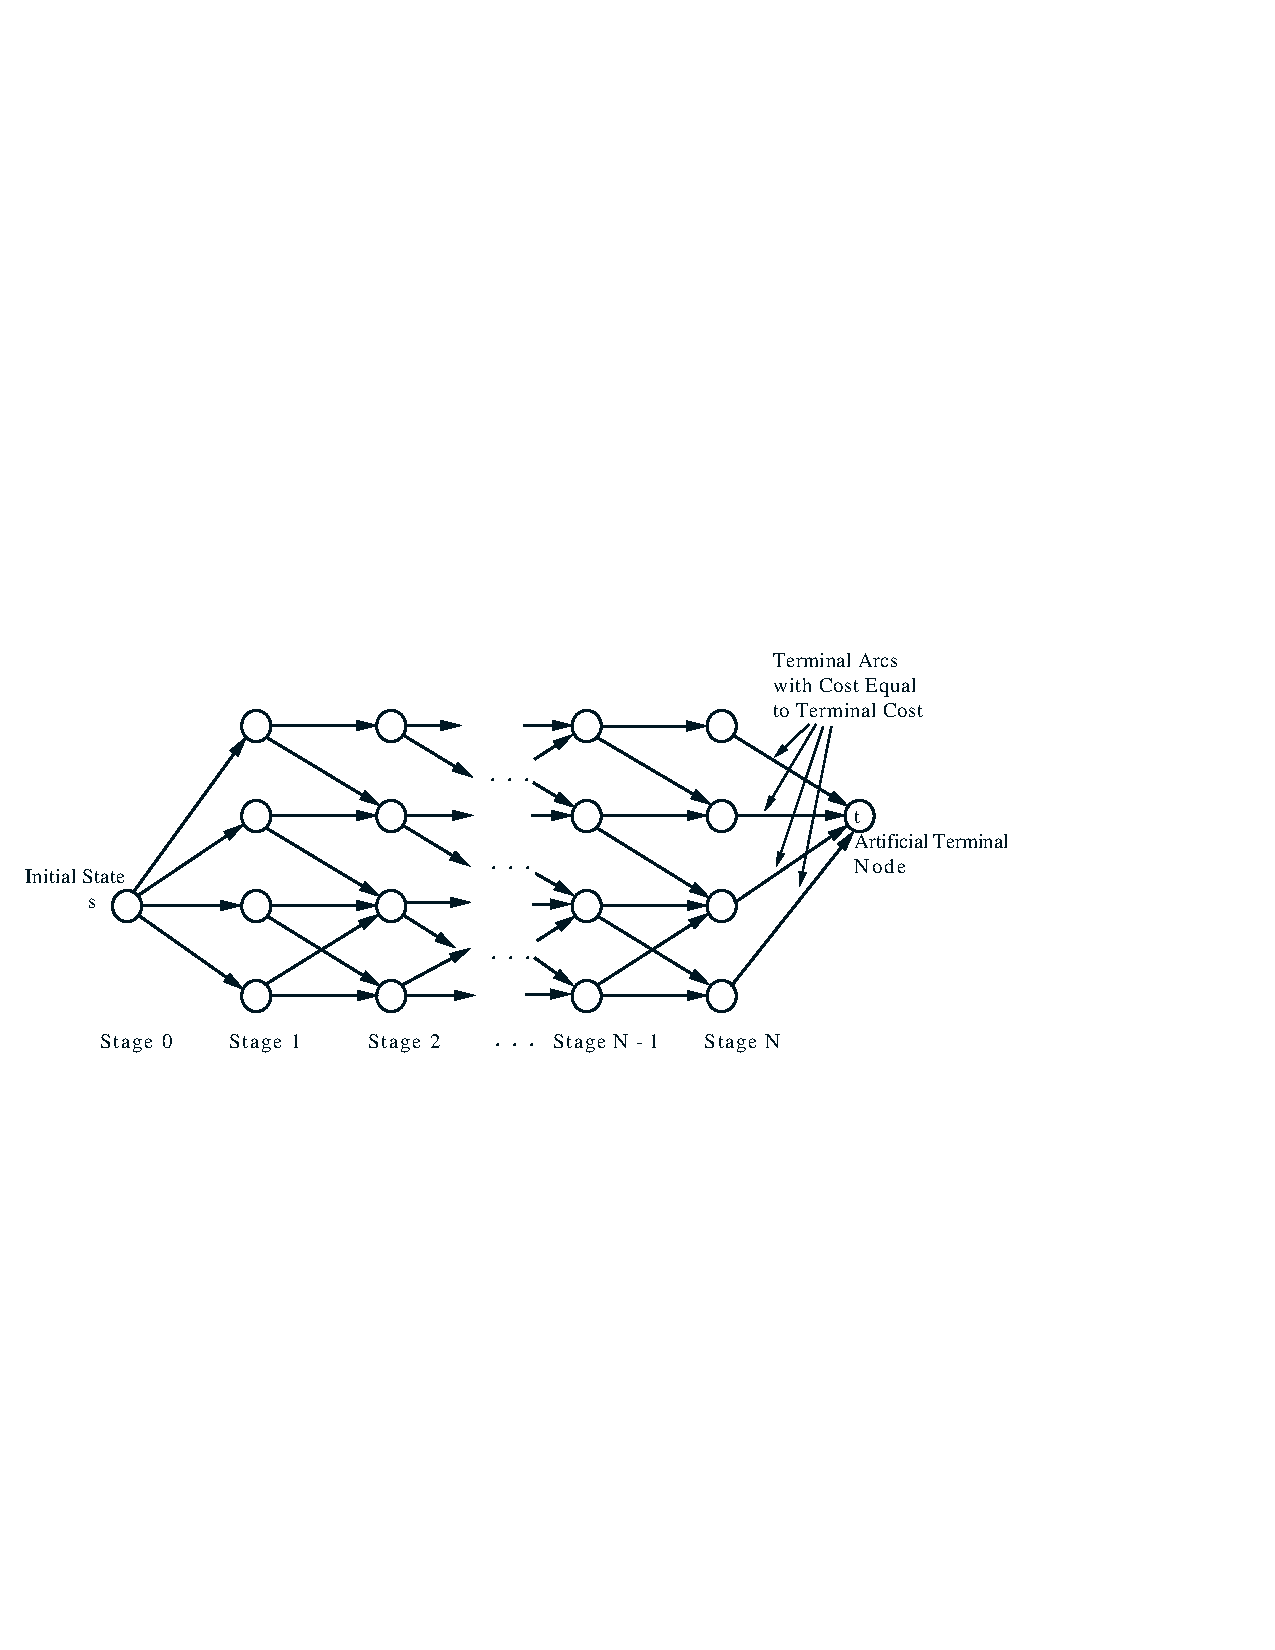
\includegraphics{dp211.pdf}}
\end{center}

Si on numérote les noeuds couche par couche, par ordre croissant de 
valeur de $k$, on obtient un \emph{réseau sans cycle et ordonné topologiquement}
(i.e., un arc $(i,j)$ ne peut exister que si $i<j$).
Dans le cas où il n'est pas nécessaire de mémoriser le numéro 
d'étape, on peut simplifier le réseau en agrégeant des noeuds.
Le réseau résultant peut ne plus être ordonné topologiquement.
Inversement, tout problème de recherche d'un plus court chemin dans
un réseau peut se formuler comme un problème de programmation dynamique déterministe (avec des coûts additifs entre étapes).

\section{Cas probabiliste}

Dans la programmation dynamique probabiliste, la décision optimale à l'étape $n$ dépend de la loi de probabilité de l'état à l'étape $n+1$.
Ainsi, nous passerons de l'étape $n$ à l'étape $n+1$, se retrouvant ainsi dans l'état $i$, avec une probabilité $p_i$.
Étant donné $S$ états à l'étape $n+1$, nous aurons $p_i \geq 0$ et
\[
\sum_{i=1}^S p_i = 1.
\]
La relation de récurrence dépend de cette loi de probabilité et de l'objectif à optimiser.

\begin{example}[Jeu de hasard]
Le jeu consiste à miser un nombre quelconque de jetons.
Si nous gagnons, nous remportons le nombre de jetons misés.
Si nous perdons, nous perdons le nombre de jetons misés.
Un statisticien croit pouvoir gagner chaque jeu avec une probabilité égale à 2/3.
Ses collègues parient avec lui qu'en misant au départ 3 jetons, il aura moins de 5 jetons après 3 parties.
Combien de jetons miser à chacune des 3 parties?

Le modèle peut se formuler comme suit:  l'étape $n$ correspond à la partie $n$, $n = 1,2,3$ ($N = 3$).
L'état $s_n$ est le nombre de jetons au début de la partie $n$, et la décision $x_n$ correspond au nombre de jetons à parier à la partie $n$.
Nous souhaitons maximiser la probabilité d'avoir au moins 5 jetons après 3 parties.
Soit $f_n(s_n,x_n)$ la probabilité de terminer avec au moins 5 jetons, étant donné que nous sommes dans l'état $s_n$ à l'étape $n$, que nous misons $x_n$ jetons et que nous effectuons des décisions optimales aux étapes $n+1,\ldots,N$.
Nous avons
\[
 f_n^*(s_n) = \max \lbrace f_n(s_n,x_n) \,|\, x_n = 0,1,\ldots,s_n \rbrace.
\]
étant donné que nous dans l'état $s_n$ à l'étape $n$ et que nous misons $x_n$ jetons, nous pouvons:
\begin{itemize}
\item
perdre et se retrouver dans l'état $s_n - x_n$ avec une probabilité 1/3;
\item
gagner et se retrouver à l'état $s_n + x_n$ avec une probabilité 2/3.
\end{itemize}
Nous avons la fonction de récurrence
\[
f_n(s_n,x_n) = \frac{1}{3}f_{n+1}^*(s_n-x_n) + \frac{2}{3}f_{n+1}^*(s_n+x_n).
\]
De plus,
\[
f_4^*(s_4) =
\begin{cases}
0 &\mbox{ si } s_4 < 5, \\
1 &\mbox{ si } s_4 \geq 5.
\end{cases}
\]
Calculons d abord $f_3^*(s_3)$ et $x_3^*$.
Nous avons le tableau
\begin{center}
\begin{tabular}{|c|c|c|c|c|c|c|c|}
\hline
$s_3$ & $x_3 = 0$ & $x_3 = 1$ & $x_3 = 2$ & $x_3 = 3$ & $x_3 = 4$ & $f_3^*(s_3)$ & $x_3^*$ \\
\hline
0 & 0 & - & - & - & - & 0 & 0 \\
\hline
1 & 0 & 0 & - & - & - & 0 & $\geq 0 $\\
\hline
2 & 0 & 0 & 0 & - & - & 0 & $\geq 0 $\\
\hline
3 & 0 & 0 & $\frac{2}{3}$ & $\frac{2}{3}$ & - & $\frac{2}{3}$ & $\geq 2$\\
\hline
4 & 0 & $\frac{2}{3}$ & $\frac{2}{3}$ & $\frac{2}{3}$ & $\frac{2}{3}$ & $\frac{2}{3}$ & $\geq 1$\\
\hline
$\geq 5$ & 1 & & & & & 1 & 0 \\
\hline
\end{tabular}
\end{center}

Voyons maintenant comment nous pouvons calculer les valeurs $f_2^*(s_2)$ et $x_2^*$, lorsque $s_2 = 3$.
Il est clair que nous devons avoir $x_2 \leq 3$. De plus,
\begin{align*}
f_2(3,0) &= \frac{1}{3}f_3^*(3) + \frac{2}{3}f_3^*(3) = \frac{2}{3}; \\
f_2(3,1) &= \frac{1}{3}f_3^*(2) + \frac{2}{3}f_3^*(4) = \frac{4}{9}; \\
f_2(3,2) &= \frac{1}{3}f_3^*(1) + \frac{2}{3}f_3^*(5) = \frac{2}{3}; \\
f_2(3,3) &= \frac{1}{3}f_3^*(0) + \frac{2}{3}f_3^*(6) = \frac{2}{3}. \\
\end{align*}
Ainsi,
\[
f_2^*(3) = \max \lbrace f_2(3,0), f_2(3,1), f_2(3,2), f_2(3,3) \rbrace = f_2(3,0).
\]
Dès lors, $x_2^* = 0$, $2$ ou $3$.
De la même façon, pour $s_2$, nous avons le tableau,
\begin{center}
\begin{tabular}{|c|c|c|c|c|c|c|c|}
\hline
$s_2$ & $x_2 = 0$ & $x_2 = 1$ & $x_2 = 2$ & $x_2 = 3$ & $x_2 = 4$ & $f_2^*(s_2)$ & $x_2^*$ \\
\hline
0 & 0 & - & - & - & - & 0 & 0 \\
\hline
1 & 0 & 0 & - & - & - & 0 & $\geq 0 $\\
\hline
2 & 0 & $\frac{4}{9}$ &  $\frac{4}{9}$ & - & - &  $\frac{4}{9}$ & $1,2$\\
\hline
3 & $\frac{2}{3}$ & $\frac{4}{9}$ & $\frac{2}{3}$ & $\frac{2}{3}$ & - & $\frac{2}{3}$ & $0,2,3$\\
\hline
4 & $\frac{2}{3}$ & $\frac{8}{9}$ & $\frac{2}{3}$ & $\frac{2}{3}$ & $\frac{2}{3}$ & $\frac{8}{9}$ & $\geq 1$\\
\hline
$\geq 5$ & 1 & & & & & 1 & 0 \\
\hline
\end{tabular}
\end{center}
Pour la première étape ($n = 1$), nous avons $s_1 = 3$, comme nous pouvons affecter 3 jetons au départ du jeu.
Ceci donne le tableau
\begin{center}
\begin{tabular}{|c|c|c|c|c|c|c|}
\hline
$s_1$ & $x_1 = 0$ & $x_1 = 1$ & $x_1 = 2$ & $x_1 = 3$ & $f_1^*(s_2)$ & $x_1^*$ \\
\hline
3 & $\frac{2}{3}$ & $\frac{20}{27}$ & $\frac{2}{3}$ & $\frac{2}{3}$ & $\frac{20}{27}$ & 1 \\
\hline
\end{tabular}
\end{center}
Dès lors
\begin{align*}
 f_1(3,0) &= \frac{1}{3}f_2^*(3) + \frac{2}{3}f_2^*(3) = \frac{2}{3}, \\
 f_1(3,1) &= \frac{1}{3}f_2^*(2) + \frac{2}{3}f_2^*(4) = \frac{20}{27}, \\
 f_1(3,2) &= \frac{1}{3}f_2^*(1) + \frac{2}{3}f_2^*(5) = \frac{2}{3}, \\
 f_1(3,3) &= \frac{1}{3}f_2^*(0) + \frac{2}{3}f_2^*(6) = \frac{2}{3},
 \end{align*}
 et par conséquent,
 \[
 f_1^*(3) = \max \lbrace f_1(3,0), f_1(3,1), f_1(3,2), f_1(3,3) \rbrace = f_1(3,1).
 \]
 Nous en déduisons
 \[
 x_1^* = 1.
 \]
La politique optimale est donc :
\begin{itemize}
\item
$x_1^* = 1$;
\item
Si nous gagnons ($s_2 = 4$), $x_2^* = 1$.
\begin{itemize}
\item
Si nous gagnons ($s_3 = 5$), $x_3^* = 0$.
\item
Si nous perdons ($s_3 = 3$), $x_3^* = 2$ ou $3$.
\end{itemize}
\item
Si nous perdons ($s_2 = 2$), $x_2^* = 1$ ou $2$.
\begin{itemize}
\item
Si nous gagnons ($s_3 = 3$ ou $4$), $x_3^* = 2$ ou $3$ (si $x_2^* = 1$) ou
$1 \leq x_3^* \leq 4$ (si $x_2^* = 2$).
\item
Si nous perdons ($s_3 = 1$ ou $0$), $x_3^* \geq 0$ (mais le pari est perdu!).
\end{itemize}
\end{itemize}
\end{example}

\begin{small}
\section{Notes}

Ce chapitre se base essentiellement sur les notes de cours de Bernard Gendron, 2007. Le lien avec les plus courts chemins est tiré du cours IFT6521 donné au département d'informatique et de recherche opérationnelle de l'Université de Montréal (Pierre L'Ecuyer, Fabian Bastin).

\end{small}


\chapter{Simulation}

\section{Introduction}

Simuler un système stochastique consiste à imiter son comportement pour estimer sa performance
Un modèle de simulation est une représentation du système stochastique permettant de générer un grand nombre d'événements aléatoires et d'en tirer des observations statistiques.

\begin{example}[Jeu de hasard]
Chaque partie consiste à tirer une pièce de monnaie jusqu'à ce que la différence entre le nombre de faces et le nombre de piles soit égale à 3.
Chaque tirage coûte 1\$, et chaque partie jouée rapporte 8\$ au joueur.
Nous aurons par exemple les jeux
\begin{itemize}
\item
 FFF: gain de 8\$-3\$=5\$;
\item
 PFPPP: gain de 8\$-5\$=3\$;
\item
 PFFPFPFPPPP: perte de 8\$-11\$=3\$.
\end{itemize}
Nous nous demandons par conséquent s'il est intéressant de jouer.
Pour répondre à cette question, nous allons simuler le jeu.
Il y a deux façons de le faire:
\begin{itemize}
\item
nous pouvons jouer pendant un certain temps sans miser d'argent;
\item
nous pouvons simuler le jeu par ordinateur.
\end{itemize}
Néanmoins, simuler une seule partie ne nous aide pas à prendre une décision.
Pour cela, il faudrait voir ce qui se passe sur un grand nombre de parties et mesurer le gain moyen
(ou la perte moyenne).

Dans cet exemple, nous pouvons définir les éléments d'un modèle de simulation comme suit
\begin{description}
\item[système stochastique]: tirages successifs;
\item[horloge]: nombre de tirages;
\item[définition de l'état du système]: $N(t)$, le nombre de faces moins le nombre de piles après $t$ tirages;
\item[événements modifiant l'état du système]: tirage de pile ou de face;
\item[méthode de génération d'événements]: génération d'un nombre aléatoire uniforme;
\item[formule de changement d'état]: $N(t+1) = N(t) + 1$, si $F$ est tirée; $N(t) - 1$, si $P$ est tirée;
\item[performance]: $8 - t$, lorsque $N(t)$ atteint +3 ou -3.
\end{description}
\end{example}

\section{Files d'attente}

\subsection{Concepts de base}

Un système de file d'attente consiste d'un ou de plusieurs serveurs
qui fournissent un service d'une certaine nature à des clients qui se
présentent, et qui sont issus d'une population donnée.
Les clients qui arrivent et trouvent tous les serveurs occupés
rejoindront (généralement) une ou plusieurs files (ou lignes) devant
les serveurs, d'où la qualification de file d'attente.
\index{file!d'attente}.
Quelques exemples de files d'attente sont repris dans la
Table~\ref{tab:queueing}.
\begin{table}[htb]
\begin{center}
\begin{tabular}{lll}
{\bf système} & {\bf Serveurs} & {\bf Clients} \\
\hline
Banque & Guichets & Clients \\
Hôpital & Docteurs, infirmiéres, lits &  Patients \\
Système informatique & Unités centrales, dispositifs I/O & Travaux \\
Manufacture & Machines, travailleurs & Composants \\
Centre d'appel & Serveurs & Appels entrants \\
\hline
\end{tabular}
\end{center}
\caption{Exemples de files d'attente}
\label{tab:queueing}
\end{table}
Le système de file d'attente est caractérisé par trois composants:
\begin{enumerate}
\item le processus d'arrivée;
\item le mécanisme de service;
\item la discipline de file.
\end{enumerate}

Spécifier le processus d'arrivée pour un système de file d'attente
revient à décrire comment les clients arrivent dans le système. Soit
$A_i$ le temps d'inter-arrivées entre les arrivées des $(i-1)^e$ et
$i^e$ clients. Si $A_1$, $A_2,\ldots$, sont supposés être des
variables i.i.d., nous dénoterons le temps d'interarrivée moyen (ou
espéré) par $E[A]$ et appellerons $\lambda = 1/E[A]$ le taux d'arrivée
des clients.

Le mécanisme de service pour un système de file d'attente est articulé
en spécifiant le nombre de serveurs (dénoté par $s$), où chaque
serveur a sa propre file ou au contraire une seule file alimente tous
les serveurs, et la distribution de probabilité des temps de service
des clients.
Soit $S_i$ le temps de service du $i^e$ client.
Si $S_1$, $S_2,\ldots$, sont des variables aléatoires i.i.d., nous dénoterons
le temps de service moyen d'un client par $E[S]$ et appelleront
$\omega = 1/E[S]$ le taux de service d'un serveur.

Nous parlerons de situation transitoire lorsque l'état du système dépend grandement de la situation initiale et du temps écoulé, et de situation d'équilibre lorsque l'état du système peut
être considéré indépendant de la situation initiale et du temps écoulé.
En situation d'équilibre, nous avons la formule de Little:
\[
 L=\lambda W,
\]
où
$L$ est le nombre moyen de clients dans le système, $\lambda$, le taux moyen d'arrivée des nouveaux clients, et $W$ le temps moyen dans le système.

\subsection{Modèle $M/M/1$}

Il s'agit du modèle de file d'attente le plus courant, avec les caractéristiques suivantes:
\begin{itemize}
\item
file d'attente: nombre infini de clients;
\item
stratégie de service: premier arrivé, premier servi (FIFO);
\item
un seul serveur;
\item
les taux d'arrivée et de service obéissent à des lois de Poisson.
De manière équivalente, le temps entre l'arrivée de deux clients successifs et le temps de service obéissent à des lois exponentielles: on parle de processus Markoviens.
\end{itemize}

La notation générale pour les modèles de file d'attente est $X/Y/s$, où $X$ représente la loi du temps d'interarrivée, $Y$ est la loi du temps de service, et $s$ donne le nombre de serveurs.

\begin{example}[File d'attente $M/M/1$]
En situation d'équilibre, plusieurs résultats analytiques (obtenus par analyse du modèle mathématique) existent.
Soit $\lambda$ le taux moyen d'arrivée et $\mu$ le taux moyen de service.
Supposons que $\lambda < \mu$
Le nombre moyen de clients dans le système vaut
\[
L = \frac{\lambda}{\mu-\lambda}.
\]
Le temps moyen d'attente dans le système vaut quant à lui
\[
W = \frac{1}{\mu-\lambda}.
\]
Il est aisé de vérifier ces résultats par simulation.
Dans le cas présent, les éléments de la simulation sont:
\begin{description}
\item[système stochastique]: file d'attente $M/M/1$;
\item[horloge] : temps écoulé;
\item[définition de l'état du système]: $N(t)$, le nombre de clients dans le système au temps $t$;
\item[événements modifiant l'état du système]: arrivée ou fin de service d'un client;
\item[formule de changement d'état] : $N(t+1) = N(t) + 1$, si arrivée; $N(t) - 1$, si fin de service.
\end{description}
Nous allons voir deux méthodes pour étudier l'evolution du système dans le temps:
\begin{itemize}
\item
 par intervalles de temps fixe;
\item
 par génération d'événement.
\end{itemize}
Nous supposerons que les valeurs des paramètres de notre système sont $\lambda$ = 3 clients par heure, et $\mu$ = 5 clients par heure.

Dans le cas d'intervalles de temps fixe, l'idée est
\begin{enumerate}
\item
faire écouler le temps d'un petit intervalle $\Delta t$;
\item
mettre à jour le système en déterminant les événements qui ont pu se produire durant l'intervalle
$\Delta t$, et recueillir l'information sur la performance du système;
\item
retourner en 1.
\end{enumerate}
Ici, les événements sont soit des arrivées, soit des départs (fins de service).
Si $\Delta t$ est suffisamment petit, nous pouvons considérer qu'il ne se produira qu'un seul événement (arrivée ou départ) durant cet intervalle de temps.

Prenons $\Delta t$ égal à 0.1 heure (6 minutes).
La probabilité qu'il y ait une arrivée durant cet intervalle de temps vaut:
\[
P_A = 1 - e^{-\lambda \Delta t} = 1-e^{-3/10} \approx 0.259.
\]
La probabilité qu'il y ait un départ durant cet intervalle de temps est:
\[
P_D = 1 - e^{-\mu \Delta t} = 1-e^{-5/10} \approx 0.393.
\]
Pour générer un événement, nous pouvons simplement tirer deux nombres aléatoires selon une loi $U[0,1]$.
Si le premier nombre est strictement plus petit que 0.259, nous aurons une arrivée.
Si le deuxième nombre est strictement inférieur à 0.393, nous considérerons un départ (si un client était en cours de service).
Ceci pourrait par exemple donner les chiffres de la Table~\ref{tab:simultime}.

\begin{table}[htbp]
\begin{center}
\begin{tabular}{|c|c|c|c|c|c|}
\hline
$t$ (min) & $N(t)$ & Nombre 1 & Arrivée & Nombre 2 & Départ \\
\hline
0 & 0 & & & & \\
\hline
6 & 1 & 0.096 & Oui & - & \\
\hline
12 & 1 & 0.569 & Non & 0.665 & Non \\
\hline
18 & 1 & 0.764 & Non & 0.842 & Non \\
\hline
24 & 1 & 0.492 & Non & 0.224 & Oui \\
\hline
30 & 0 & 0.950 & Non & - & \\
\hline
36 & 0 & 0.610 & Non & - & \\
\hline
42 & 1 & 0.145 & Oui & - & \\
\hline
48 & 1 & 0.484 & Non & 0.552 & Non \\
\hline
54 & 1 & 0.350 & Non & 0.590 & Non \\
\hline
60 & 0 & 0.430 & Non & 0.041 & Oui \\
\hline
\end{tabular}
\caption{Simulation par intervalles de temps fixe.}
\label{tab:simultime}
\end{center}
\end{table}
D'après cet exemple, il est possible d'estimer les performances du système.
Que se passe-t-il si nous voulons mesurer $W$, le temps moyen passé dans le système?
Nous avons deux clients qui sont entrés dans le système et chacun y est resté 18 minutes ou 0.3 heures, aussi peut-on estimer $W$ par 0.3.
Pourtant, la vraie valeur est $W = 1/(\mu-\lambda) = 0.5$.
Il faudrait un \'echantillon beaucoup plus grand, et ce d'autant plus que nous devrions simuler le système en état d'équilibre.

La génération d'événement peut se résumer comme suit:
\begin{enumerate}
\item
faire écouler le temps jusqu'au prochain événement;
\item
mettre à jour le système en fonction de l'événement qui vient de se produire et générer aléatoirement le temps jusqu'au prochain événement; recueillir l'information sur la performance du système;
\item
retourner à 1.
\end{enumerate}
Nous pourrions ainsi obtenir la suite d'événements reprise dans la Table~\ref{tab:simulevents}.

\begin{table}[htbp]
\begin{center}
\begin{tabular}{|c|c|c|c|c|c|c|}
\hline
$t$ (min) & $N(T)$ & Temps & Temps &  Prochaine & Prochain & Prochain \\
& & d'interarrivée & de service & arrivée & départ & événement \\
\hline
0 & 0 & 2.019 & - & 2.019 & - & Arrivée \\
\hline
2.019 & 1 & 16.833 & 13.123 & 18.852 & 15.142 & Départ \\
\hline
15.142 & 0 & - & - & 18.852 & - & Arrivée \\
\hline
18.852 & 1 & 28.878 & 22.142 & 47.730 & 40.994 & Départ \\
\hline
40.994 & 0 & - & - & 47.730 & - & Arrivée \\
\hline
47.730 & 1 & & & & & \\
\hline
\end{tabular}
\caption{Simulation par événements.}
\label{tab:simulevents}
\end{center}
\end{table}

Si nous considérons une simulation comportant l'arrivée de 10000 clients, les résultats montrent que:
\begin{itemize}
\item
 le nombre moyens de clients dans le système est $L \approx 1.5$;
\item
 le temps moyen dans le système est $W \approx 0.5$.
\end{itemize}

Remarque: des résultats analytiques existent pour des modèles simples (comme $M/M/1$), mais pas pour des files d'attente plus complexes.
\end{example}

\section{Simulation à événements discrets}

L'approche s'est imposée dans nombre de problèmes de simulations.
Le principe général est résumé dans l'ordinogramme de la Figure~\ref{fig:sim_flowchart}.

\begin{figure}[htb]

\tikzstyle{decision} = [diamond, draw, fill=blue!20,
    text width=2.5cm, text badly centered, node distance=2.5cm, inner sep=0pt]
\tikzstyle{block} = [rectangle, draw, fill=blue!20,
    text width=2.5cm, text centered, rounded corners, minimum height=4em]
\tikzstyle{line} = [draw, very thick, color=black!50, -latex']
\tikzstyle{cloud} = [draw, ellipse,fill=yellow!20, node distance=2.5cm,
    minimum height=2em]

\begin{center}
\begin{tikzpicture}[scale=2, node distance = 3cm, auto]
    % Place nodes
    \node [block] (init) {Initialisation};
    \node [text width=2.2cm, cloud, left of=init, node distance=4.0cm] (clock) {Horloge de simulation mise à 0};
    \node [text width=2.5cm, cloud, right of=init, node distance=4.0cm] (system) {Planification du ou des premiers(s) événement(s)};
    \node [text width=2.1cm, block, below of=init, node distance=3.0cm] (event) {Gestion de l'événement actuel};
    \node [text width=2.1cm, block, below of=event, node distance=3.0cm] (schedule) {Planification du ou des événements en découlant.};
    \node [block, left of=schedule, node distance=5.0cm] (update) {Dépilement du prochain événement et avancement de l'horloge de simulation};
    \node [text width=2.1cm, decision, below of=schedule, node distance=4.0cm] (decide) {Liste d'événements vide?};
    \node [block, below of=decide, node distance=3.5cm] (stop) {Arrêt};
    % Draw edges
    \path [line] (init) -- (event);
    \path [line] (event) -- (schedule);
    \path [line] (schedule) -- (decide);
    \path [line] (decide) -| node [near start, color=black] {non} (update);
    \path [line] (update) |- (event);
    \path [line] (decide) -- node [, color=black] {oui}(stop);
    \path [line,dashed] (clock) -- (init);
    \path [line,dashed] (system) -- (init);
\end{tikzpicture}
\caption{Schéma d'une simulation à événements discrets.}
\label{fig:sim_flowchart}
\end{center}
\end{figure}

\begin{small}
\section{Notes}

Ce chapitre se base essentiellement sur les notes de cours de Bernard Gendron, 2007.
Pour plus de détails sur la simulation à événements discrets, nous renvoyons le lecteur aux notes du cours IFT3245, du même auteur: .

\end{small}


\backmatter

\chapter{Annexe}

\section{Logiciels d'optimisation}

\subsection{IOR Tutorial}

Le logiciel IOR Tutorial, qui accompagne le livre {\sl Introduction to Operational Research} \citep{HillLieb01} est disponible gratuitement à l'adresse \url{http://highered.mcgraw-hill.com/sites/0073017795/student_view0/ior_tutorial.html}.
Le logiciel est fourni sous la forme d'un exécutable sous l'environnement Microsoft Windows, et comme archive Java pour les autres plate-formes.
Il est par conséquent utilisable sur la majorité des systèmes actuels.
Le logiciel est intéressant pour rapidement tester des programmes d'optimisation simples, mais ne peut être considéré comme un solveur à part entière.
Son interface graphique le rend néanmoins adapté pour une expérimentation rapide avec les exemples introduits dans lecours.

\subsection{GAMS}

% Développer la dualité

GAMS est l'acronyme de {\bf G}eneralized {\bf A}lgebric {\bf M}odeling {\bf S}ystem.
Il s'agit avant tout d'un langage servant à la formulation et à la résolution de modèle de programmation mathématique.
En pratique, il s'agit d'un paquetage intégré qui permet de
\begin{itemize}
\item
spécifier la structure du modèle d'optimisation;
\item
spécifier et calculer les données qui entrent dans le modèle;
\item
résoudre ce modèle;
\item
produire un rapport sur un modèle;
\item
conduire une analyse comparative.
\end{itemize}
GAMS peut être téléchargé à l'adresse \url{http://www.gams.com}.
La licence de GAMS et des solveurs académique est passablement élevés, toutefois il est utilisable de manière gratuite en version de démonstration, ce qui permettra d'illustrer certains concepts de base du cours.

Sous des environnements de type UNIX (incluant Mac OS X et la majorité des distributions Linux), GAMS s'utilise uniquement en ligne de commande.
Sous Microsoft Windows, il dispose d'une interface graphique.

\subsubsection{Formulation d'un problème simple}

\begin{example}
\label{gams_simple}
Considérons le problème d'optimisation linéaire
\begin{align*}
\max_x \ & 109 x_1 + 90 x_2 + 115 x_3 \\
\st & x_1 + x_2 + x_3 \leq 100; \\
& 6x_1 + 4x_2 + 8x_3 \leq 500; \\
& x_1,\ x_2,\ x_3 \geq 0.
\end{align*}
Le fichier GAMS décrivant se problème est constitué des parties suivantes:
\begin{enumerate}
\item
spécification des variables;
\item
spécification des équations:
\begin{itemize}
\item
déclaration;
\item
spécification de la structure algébrique;
\end{itemize}
\item
définition du modèle;
\item
définition de la méthode de résolution.
\end{enumerate}
Ce problème peut être formulé sous GAMS comme suit:
\begin{verbatim}
VARIABLES
  Z               Variable Z;

POSITIVE VARIABLES
  X1              Variable X1
  X2              Variable X2
  X3              Variable X3;

EQUATIONS
  Equation1       Equation 1
  Equation2       Equation 2
  Equation3       Equation 3;

Equation1..
  Z =E= 109*X1 + 90*X2 + 115*X3;

Equation2..
  X1 + X2 + X3 =L= 100;

Equation3..
  6*X1 + 4*X2 + 8*X3 =L= 500;

MODEL Example1 /ALL/;

SOLVE Example1 USING LP MAXIMIZING Z;
\end{verbatim}
Remarquons d'ores et déjà que chaque instruction se termine par un point-virgule.
Leur omission produit une erreur de compilation.
Détaillons les instructions.
\end{example}

\subsubsection{Spécification des variables}

GAMS exige que les variables soient identifiées.
Dans l'exemple précédent, nous avons les variables \verb|Z|, \verb|X1|, \verb|X2|, \verb|X3|:
\begin{verbatim}
VARIABLES
  Z               Variable Z;

POSITIVE VARIABLES
  X1              Variable X1 (Optional Text)
  X2              Variable X2
  X3              Variable X3;
\end{verbatim}
Pour tout modèle construit avec GAMS, il convient d'identifier l'objectif à l'aide d'une variable, ici \verb|Z|. Autrement dit,
\[
\max_x c^Tx
\]
devient
\begin{align*}
\max\ & z\\
\st\ & z=c^Tx, \\
 & Z=CX.
\end{align*}
Les noms de variables peuvent avoir jusqu'à 31 caractères.
Il est également possible de spécifier plus précisément le type des variables:\\
\begin{tabular}{ll}
\verb|VARIABLE| & variables non restreintes \\
\verb|POSITIVE VARIABLE| & variables non négatives \\
\verb|NEGATIVE VARIABLE| & variables non positives \\
\verb|BINARY VARIABLE| & variables binaires (dans $\lbrace 0, 1\rbrace$) \\
\verb|INTEGER VARIABLE| & variables entières (naturelles)
\end{tabular}

\subsubsection{Dénomination des équations}

La spécification d'une équation consiste en deux parties.
Il convient tout d'abord de déclarer ces équations: GAMS exige du modélisateur de nommer chaque équation à l'oeuvre dans le modèle.
Dans l'exemple, les équations sont déclarées après le mot-clé \verb|EQUATIONS|
\begin{verbatim}
EQUATIONS
  Equation1       Equation 1
  Equation2       Equation 2
  Equation3       Equation 3;
\end{verbatim}
Comme pour les variables, le nom d'une équation peut prendre jusqu'à 31 caractères.
A droite du nom de l'équation figure un (bref) texte d'explications.

Il nous faut de plus spécifier la structure algébrique: après avoir nommé les équations, la structure algébrique exacte doit être spécifiée en utilisant la notation \verb|..|:
\begin{verbatim}
Equation1..
  Z =E= 109*X1 + 90*X2 + 115*X3;

Equation2..
  X1 + X2 + X3 =L= 100;

Equation3..
  6*X1 + 4*X2 + 8*X3 =L= 500;
\end{verbatim}
La forme algébrique exige l'utilisation d'une syntaxe speciale afin de définir la forme exacte de l'équation:\\
\begin{tabular}{ll}
\verb|=E=| & contrainte d'égalité \\
\verb|=L=| & inférieur ou égal \\
\verb|=G=| & supérieur ou égal
\end{tabular}

\subsubsection{Spécification du modèle}

Le mot-clé \verb|MODEL| est utilisé pour identifier les modèles à résoudre.
Il convient de
\begin{enumerate}
\item
donner un nom au modèle (par exemple \verb|Example1|);
\item
spécifier les équations à inclure, entre des barres italiques \verb|/ /|.
\end{enumerate}
Ceci donne pour notre exemple
\begin{verbatim}
MODEL Example1 /ALL/;
\end{verbatim}
Nous pourrions aussi avoir
\begin{verbatim}
MODEL Example1 /Equation1, Equation2/;
\end{verbatim}

\subsubsection{Spécification du solveur}

Le mot-clé \verb|SOLVE| indique à GAMS d'appliquer un solveur au modèle nommé, en utilisant les données définies juste avant l'instruction \verb|SOLVE|.
Ainsi, dans notre exemple, nous avions:
\begin{verbatim}
SOLVE Example1 USING LP MAXIMIZING Z;
\end{verbatim}
Si nous avions affaire à un problème linéaire de minimisation, nous pourrions écrire
\begin{verbatim}
SOLVE Example1 USING LP MINIMIZING Z;
\end{verbatim}
En place de \verb|LP|, nous devrions écrire \verb|MIP| pour traiter un problème de programmation entière mixte:
\begin{verbatim}
SOLVE Example1 USING MIP MAXIMIZING Z;
\end{verbatim}
De même, nous spécifierons un problème non-linéaire avec le mot-clé \verb|NLP|:
\begin{verbatim}
SOLVE Example1 USING NLP MAXIMIZING Z;
\end{verbatim}

\subsubsection{Rapport de solution}

A la fin de l'exécution, GAMS produit un rapport indiquant la solution trouvée, la valeur de la fonction objectif en cette solution, ainsi que différentes informations permettant d'analyser le comportement de l'algorithme d'optimisation, et diverses propriétés du problème en cours d'étude.
En particulier, le résumé de rapport donne le nombre total de cas non optimaux, non réalisables et non bornés rencontrés.
\begin{verbatim}
**** REPORT SUMMARY :        0     NONOPT
                             0 INFEASIBLE
                             0  UNBOUNDED
\end{verbatim}

L'information sur les solutions peut être affichée de différentes manières:
\begin{enumerate}
\item
sortie standard de GAMS;
\item
utilisation des commandes \verb|DISPLAY|;
\item
rappports additionels sur base des valeurs des solutions.
\end{enumerate}

La sortie standard de GAMS présente la solution sous forme d'un tableau, qui dans le cas de l'exemple est:
\begin{verbatim}

                       LOWER     LEVEL     UPPER    MARGINAL

---- EQU Equation1       .         .         .        1.000      
---- EQU Equation2      -INF    100.000   100.000    52.000      
---- EQU Equation3      -INF    500.000   500.000     9.500      

  Equation1  Equation 1
  Equation2  Equation 2
  Equation3  Equation 3

                       LOWER     LEVEL     UPPER    MARGINAL

---- VAR Z              -INF   9950.000     +INF       .         
---- VAR X1              .       50.000     +INF       .         
---- VAR X2              .       50.000     +INF       .         
---- VAR X3              .         .        +INF    -13.000      
\end{verbatim}

Le point simple ``.'' représente un zéro, tandis que \verb|INF| représente l'infini.

\subsubsection{Sommations}

La notation mathématique $\sum_j x_j$ se traduira par
\begin{verbatim}
SUM(j,x(j))
\end{verbatim}
En d'autres termes, nous avons la syntaxe
\begin{verbatim}
SUM( index of summation, names(index))
\end{verbatim}
Il est possible d'imbriquer les sommations. Ainsi, $\sum_j \sum_i x{ji}$ donnera
\begin{verbatim}
SUM(j,SUM(i,x(j,i))
\end{verbatim}
ou encore
\begin{verbatim}
SUM((j,i),x(j,i))
\end{verbatim}

\subsubsection{Définition d'ensemble}

Spécifier les variables une à une est vite fastidieux, pour ne pas dire irréaliste (par exemple si nous avons un million de variables), c'est pourquoi en modélisation algébrique, nous utilisons des indices.
GAMS met à disposition le mot clé \verb|SET| pour définir des ensembles, parcouru par un indice spécifié juste avant:
\begin{verbatim}
SET   ItemName   optional explanatory text for item
  / element1   optional explanatory text for element,
    element2   optional explanatory text for element /
\end{verbatim}
Par exemple,
\begin{verbatim}
SET   i   index /1*10/
\end{verbatim}
défini l'ensemble $\lbrace 1,2,\ldots,10 \rbrace$, qui peut être parcouru avec l'indice $i$.
Il est possible d'associer un autre indice  au même ensemble  au moyen de la commande \verb|ALIAS|, par exemple
\begin{example}
ALIAS (i,j);
\end{example}
permet d'utiliser $j$ au lieu de $i$.
Cette commande est utile par exemple pour traduire une contrainte de la forme
\[
x_{ij} + x_{ji} = 1,\ i = 1,\ldots,n,\ j=1,\ldots,n,
\]
$j$ et $i$ doivent indicer le même ensemble, mais écrire
\begin{verbatim}
SET  i  / 1*10 /
          j  / 1*10 /
\end{verbatim}
mènerait GAMS à considérer $i$ et $j$ comme indexant deux ensembles.

\subsubsection{Entrée de données}

Les données sont entrées au moyen de quatre différents types de commandes GAMS:
\begin{description}
\item[SCALAR], pour les éléments ne dépendant pas d'ensembles; 
\item[PARAMETERS], pour les éléments qui sont des vecteurs;
\item[TABLES], pour des éléments de deux dimensions ou plus;
\item[PARAMETERS], en affectation directe.
\end{description}
La manière la plus simple d'entrée des données est l'emploi de la commande \verb|SCALAR|, qui prend la syntaxe suivante dans le format basique:
\begin{verbatim}
SCALAR  ItemName  optional text   / value /;
\end{verbatim}
Dans le cas de vecteurs, nous utiliserons la syntaxe
\begin{verbatim}
PARAMETER  ItemName(Set)  optional text;
   / element1  value,
     element2  value  /;
\end{verbatim}
Pour les entrées multidimensionnelles, nous aurons
\begin{verbatim}
TABLE  ItemName(set1dep,set2dep)  optional text
               set2elem1    set2elem2
set1element1    value11      value12
set1element2    value12      value22    ;
\end{verbatim}
Plutôt que d'utiliser des constantes, nous pouvons affecter les valeurs au moyen d'expressions mathématiques:
\begin{verbatim}
PARAMETER  ItemName(set1dep,set2dep)  optional text;
           ItemName(set1dep,set2dep) = some expression;
\end{verbatim}
L'indice \verb|set2dep| est optionnel.

L'exemple~\ref{gams_simple} peut ainsi se reformuler comme
\begin{verbatim}
SETS
  i               Variables / X1, X2, X3 /;

PARAMETERS
  c(i)            Costs / X1 109
                          X2 90
                          X3 115 /

  a(i)            Coeff / X1 6
                          X2 4
                          X3 8 /;

VARIABLES
  Z               Variable Z;

POSITIVE VARIABLES
  x(i)            Variables;

EQUATIONS
  Equation1       Equation 1
  Equation2       Equation 2
  Equation3       Equation 3;

Equation1..
  Z =E= sum(i, c(i)*x(i));

Equation2..
  sum(i, x(i)) =L= 100;

Equation3..
  sum(i, a(i)*x(i)) =L= 500;

MODEL Example1 /ALL/;

SOLVE Example1 USING LP MAXIMIZING Z;
\end{verbatim}

%\subsection{NEOS Server}

\subsection{Autres logiciels}

Les solutions logiciels retenues sont loin d'être les seules envisageables, et les choix sont volontairement orientés afin de répondre aux objectifs d'un cours d'introduction, mais ne représentent pas forcément un choix optimal.
Il existe d'autres langages de modélisation intéressant (on pensera par exemple à AMPL), d'autres solveurs commerciaux ou gratuits.
Nous nous désinteresserons cependant des solveurs intégrés dans les tableurs, les algorithmes proposés par défaut dans ceux-ci étant en général de faible qualité, en particulier en optimisation non-linéaire, et limités dans le nombre de variables qui peuvent être traités.
Il est toutefois bon de noter que des outils existent pour importer/exporter des données entre un tableur et des outils tels que GAMS.

\begin{small}
\section{Notes}

La section sur GAMS s'inspire partiellement du cours {\sl Applied Mathematical Programming} donné par Bruce A. McCarl à l'Université Texas A\&M.

\end{small}

%\pagebreak
\addcontentsline{toc}{chapter}{Bibliographie}
%\nocite{*}
\makeatletter
\bibliographystyle{myplain}
\bibliography{refs}
\@mkboth{Bibliography}{Bibliographie}
\makeatother

\vspace{\stretch{1}}

\end{document}
